\chapter{Experimental Results and Analysis}\label{ch:results}

This chapter presents the empirical evaluation of the exploration environment described in the previous chapter. It first establishes the shared experimental setup and rationale underlying all experiments, then validates the accuracy of the underlying projection and clustering methods on previously unseen data. The remaining sections evaluate each of the plugin's navigation operations individually. The datasets, analysis scripts, and results referenced throughout this chapter are publicly available in the project repository \cite{davidgh2026nels}, under the \texttt{datasets} and \texttt{analysis} directories respectively.

\section{Evaluation parameters}\label{sec:5.1}

Following the implementation and its limitations described in the previous chapter, this evaluation focuses on whether the generated trajectories exhibit interpretable, continuous, and reproducible changes under controlled experimental conditions. To make comparisons between operations and parameter settings meaningful, all experiments use a standardized image-generation configuration.

Every image-generation experiment reported in this chapter uses the same sampling parameters. This ensures that observed differences between experimental conditions are primarily due to the navigation operations rather than to changes in the generation setup. All images are generated at a resolution of 512x512 pixels using the Euler sampler, the \texttt{simple} scheduler, a classifier-free guidance scale of 8.0, and full denoising with a denoising strength of 1.0. The model and text encoder correspond to the configuration introduced in \hyperref[sec:4.5]{Section~4.5}.

The sampling seed is not configured independently. Instead, it is derived from the same fixed seed used to select the loaded dataset subset, \texttt{42}, and remains constant across all experiments in this chapter. This controls the stochastic component of the generation process and prevents newly sampled noise from introducing an additional source of variation when images and consecutive trajectory steps are compared.

The number of denoising steps was selected empirically during preliminary testing, comparing image quality and how well the generated images represented the prompt's semantics at different steps. Based on these observations, 20 steps were adopted as the fixed setting for all image-generation experiments reported in this chapter, keeping the generation time per image at a minimum while still producing reliable results.

\FloatBarrier
\section{Projection and cluster structure}\label{sec:5.2}

\hyperref[sec:4.6]{Section~4.6} introduced the three projection strategies \texttt{classic}, \texttt{two\_pass}, and \texttt{parametric} and compared their canonical fits using ImageNet-1k datasets constructed from the same corpus of 1.000 class-label prompts. However, that comparison does not show how accurately each strategy handles previously unseen points at runtime. The present section therefore evaluates three aspects of runtime performance: the accuracy with which new points are placed in the existing projection, the accuracy of their assigned cluster labels, and whether the same local neighborhood is retained after projecting a new point, regardless of whether its projected coordinates are accurate. For each strategy, a subset of prompts is withheld during dataset construction and subsequently processed using the corresponding runtime projection and cluster-assignment procedures. The resulting coordinates and cluster assignments are then compared with those obtained from a complete canonical fit that includes the held-out prompts to reveal differences.

The 1.000 ImageNet-1k prompts are divided deterministically into 800 training prompts and 200 held-out prompts using a fixed random seed. Because the split is generated from newly reconstructed prompt text rather than from the row order of the existing datasets, the identifiers of the held-out samples are recovered by matching their exact text against the samples stored in the existing \texttt{imagenet1k\_labels\_classic} dataset. A separate 800-prompt training dataset is then created for each projection strategy. All datasets use the same CLIP encoder, canonical UMAP parameters, and clustering configuration as the corresponding full 1.000-point comparison datasets. The number of training samples is therefore the only systematic difference between each reduced training dataset and its full reference dataset.

For the \texttt{two\_pass} strategy, the runtime projection models are trained on a deterministic subset of the canonical dataset. To preserve the same 50 percent subset proportion used in the existing comparison dataset, 400 of the 800 training points are selected for the primary evaluation. For each strategy, the corresponding existing 1.000-point dataset serves as the reference, since its canonical fit already contains the 200 held-out prompts.

For each strategy, the 200 held-out prompts' already-encoded compact embeddings are reused directly, since they are byte-identical across all three comparison datasets, and are pushed through that strategy's runtime projection and cluster-assignment functions. For \texttt{classic}, this means transforming through the saved canonical UMAP models and predicting cluster assignment via the cluster-space UMAP together with HDBSCAN's approximate-prediction mechanism. \texttt{parametric} uses the same two steps through its trained neural encoder, since it maintains no separate runtime model. \texttt{two\_pass} instead projects positions through its smaller runtime UMAP models, while cluster assignment uses the FAISS-based cosine-similarity vote described in \hyperref[sec:4.6]{Section~4.6}.

Because the runtime and reference projections are produced by independently fitted UMAP models, their coordinates cannot be compared directly. Even when both embeddings preserve a similar structure, their coordinate systems may differ by translation, rotation, reflection, and uniform scaling. Coordinate accuracy is therefore evaluated after a scaled Procrustes alignment \cite{dupre2021procrustes}, a standard procedure for aligning two corresponding point sets. The 800 training prompts serve as landmarks because their coordinates are available in both the runtime projection and the full reference projection. The orthogonal transformation is estimated using \texttt{scipy.linalg.orthogonal\_procrustes}, while centering and uniform scaling are applied explicitly. For each held-out point, the coordinate error is then defined as the Euclidean distance between its aligned runtime position $p_{\text{aligned}}$ and its reference position $g$:
\[
d = \lVert p_{\text{aligned}} - g \rVert.
\]
The errors of the 200 held-out prompts are summarized by their mean, median, and standard deviation, separately for the two- and three-dimensional projections.

Cluster-assignment accuracy is evaluated using the Adjusted Rand Index (ARI) \cite{hubert_comparing_1985}, comparing each held-out point's cluster label predicted by the strategy's runtime procedure against its ground-truth cluster label from the corresponding full 1.000-point dataset. The ARI compares two clusterings by considering all pairs of samples and determines whether each pair is assigned to the same cluster or to different clusters in both labelings. It then subtracts the amount of agreement expected by chance from this score. This makes the measure independent of the numerical identifiers assigned to individual clusters, which is essential because HDBSCAN and the \texttt{two\_pass} voting procedure may represent the same underlying grouping with different cluster numbers. An ARI of 1 indicates identical cluster assignments, a value near 0 indicates agreement comparable to random labeling, and negative values indicate agreement below chance. Noise points are treated as members of a separate label category. The score is computed with \texttt{sklearn.metrics.adjusted\_rand\_score}. In addition, noise agreement is reported as the proportion of held-out points for which the predicted noise status matches the reference noise status.

The third aspect, neighbor recall, is evaluated next. For each held-out prompt, a reference neighborhood $N_i^{\text{raw}}$ is first defined directly in the compact embedding space. It consists of the $k = 32$ most similar samples among the 800 training prompts, measured by cosine similarity. Because this step is performed before dimensionality reduction, the resulting neighborhood is independent of the projection strategy.

Two projected neighborhoods are then compared with the same compact-space reference. The first, labeled \texttt{subset} represents the strategy's runtime behavior. The held-out point is projected using the runtime model fitted on the corresponding 800-point training dataset. Where the runtime model defines an independent coordinate system, as in the \texttt{two\_pass} strategy, its output is first transformed into the coordinate frame of that same 800-point dataset's own stored training-point positions, using the Procrustes alignment described above. The 32 nearest training samples are then identified in the aligned two- or three-dimensional space.

The second variant, labeled \texttt{canonical} in the underlying results, referred to here as the \textbf{ground-truth} variant, is derived from the corresponding full 1.000-point reference dataset. Since both the held-out prompts and the 800 training prompts were included in its full fit, their stored two- and three-dimensional coordinates can be compared directly. No runtime projection or alignment is required. The resulting neighborhood therefore reflects the structure preserved by the complete UMAP fit itself rather than by an additional runtime approximation.

Neighbor recall at $k$ is defined as
\[
\text{recall@}k = \frac{1}{n}\sum_{i=1}^{n} \frac{\lvert N_i^{\text{raw}} \cap N_i^{\text{proj}} \rvert}{k},
\]
where $n = 200$ is the number of held-out prompts and $N_i^{\text{proj}}$ is the neighborhood obtained from either the runtime or the ground-truth variant. The metric represents the average proportion of compact-space neighbors that remain among the $k$ nearest neighbors after projection. The ground-truth score, derived entirely from the complete 1.000-point canonical fit, measures the neighborhood information lost through dimensionality reduction alone. The difference between the runtime score, computed from the reduced 800-point fit, and the ground-truth score then estimates the additional loss introduced specifically by the strategy's runtime approximation of fitting on fewer points and projecting the held-out point out-of-sample.

\begin{table}[htbp]
\centering
\caption{Held-out accuracy per strategy. Neighbor recall is reported as runtime-model / ground-truth-model}
\label{tbl:held-out-accuracy}
\resizebox{\textwidth}{!}{%
\begin{tabular}{|l|c|c|c|c|c|c|}
\hline
\textbf{Strategy} & \textbf{Coord. err. 2D} & \textbf{Coord. err. 3D} & \textbf{Cluster ARI} & \textbf{Noise agr.} & \textbf{Recall@32 2D} & \textbf{Recall@32 3D} \\
& \textbf{(mean/med./SD)} & \textbf{(mean/med./SD)} & & & & \\
\hline
\texttt{classic} & 1.228 / 0.798 / 1.056 & 1.120 / 0.998 / 0.569 & 0.679 & 0.985 & 0.390 / 0.390 & 0.449 / 0.434 \\
\hline
\texttt{two\_pass} & 36.161 / 38.527 / 5.364 & 50.751 / 51.785 / 4.710 & 0.679 & 0.985 & 0.219 / 0.390 & 0.287 / 0.434 \\
\hline
\texttt{parametric} & 1.383 / 1.067 / 1.240 & 1.014 / 0.937 / 0.532 & 0.222 & 0.780 & 0.288 / 0.386 & 0.370 / 0.421 \\
\hline
\end{tabular}%
}
\end{table}

Because \texttt{classic} and \texttt{two\_pass} share the same reference fit, their ground-truth cluster labels and noise assignments are identical. Their runtime procedures differ, however. As described above, \texttt{classic} reuses the original fitted projection and clustering models, whereas \texttt{two\_pass} relies on a separately trained runtime projection and a FAISS-based voting procedure for cluster assignment.

Even after Procrustes alignment and scale correction, the coordinate error of \texttt{two\_pass} remains approximately 30 times larger than that of \texttt{classic}, visible in \hyperref[fig:dataset-strategy-position-scatter]{Figure~\ref*{fig:dataset-strategy-position-scatter}}. Its neighbor recall is also close to half the value obtained from the corresponding ground-truth fit. These findings indicate that the separately fitted runtime UMAP model provides a substantially weaker approximation of the ground-truth projection than the direct model reuse employed by \texttt{classic}. By contrast, the FAISS-based cluster-assignment procedure used by \texttt{two\_pass} reproduces the ground-truth cluster labels with approximately the same accuracy as HDBSCAN's approximate prediction in \texttt{classic}.
The cluster ARI obtained by \texttt{parametric} is considerably lower than that of the other two strategies. This result is consistent with its ground-truth fit producing a substantially different cluster structure from the shared reference fit used by \texttt{classic} and \texttt{two\_pass}.

The comparison is based on a relatively small corpus consisting of 800 training prompts and 200 held-out prompts. Runtime projections based on UMAP may benefit from larger and more representative training sets, meaning that the relative disadvantage observed for \texttt{two\_pass} cannot necessarily be transferred directly to the substantially larger datasets. A direct evaluation at that scale was not feasible with the available hardware, making this small-corpus experiment the only direct assessment of runtime projection accuracy conducted in this work.

Within this held-out evaluation, \texttt{classic} most closely reproduces the ground-truth reference fit. The ground-truth geometry of \texttt{parametric} differs most strongly from those of the other two strategies, while \texttt{two\_pass} provides the least accurate runtime coordinate approximation. Its cluster-assignment procedure nevertheless performs at a level comparable to that of \texttt{classic}.

\begin{figure}[htbp]
\centering
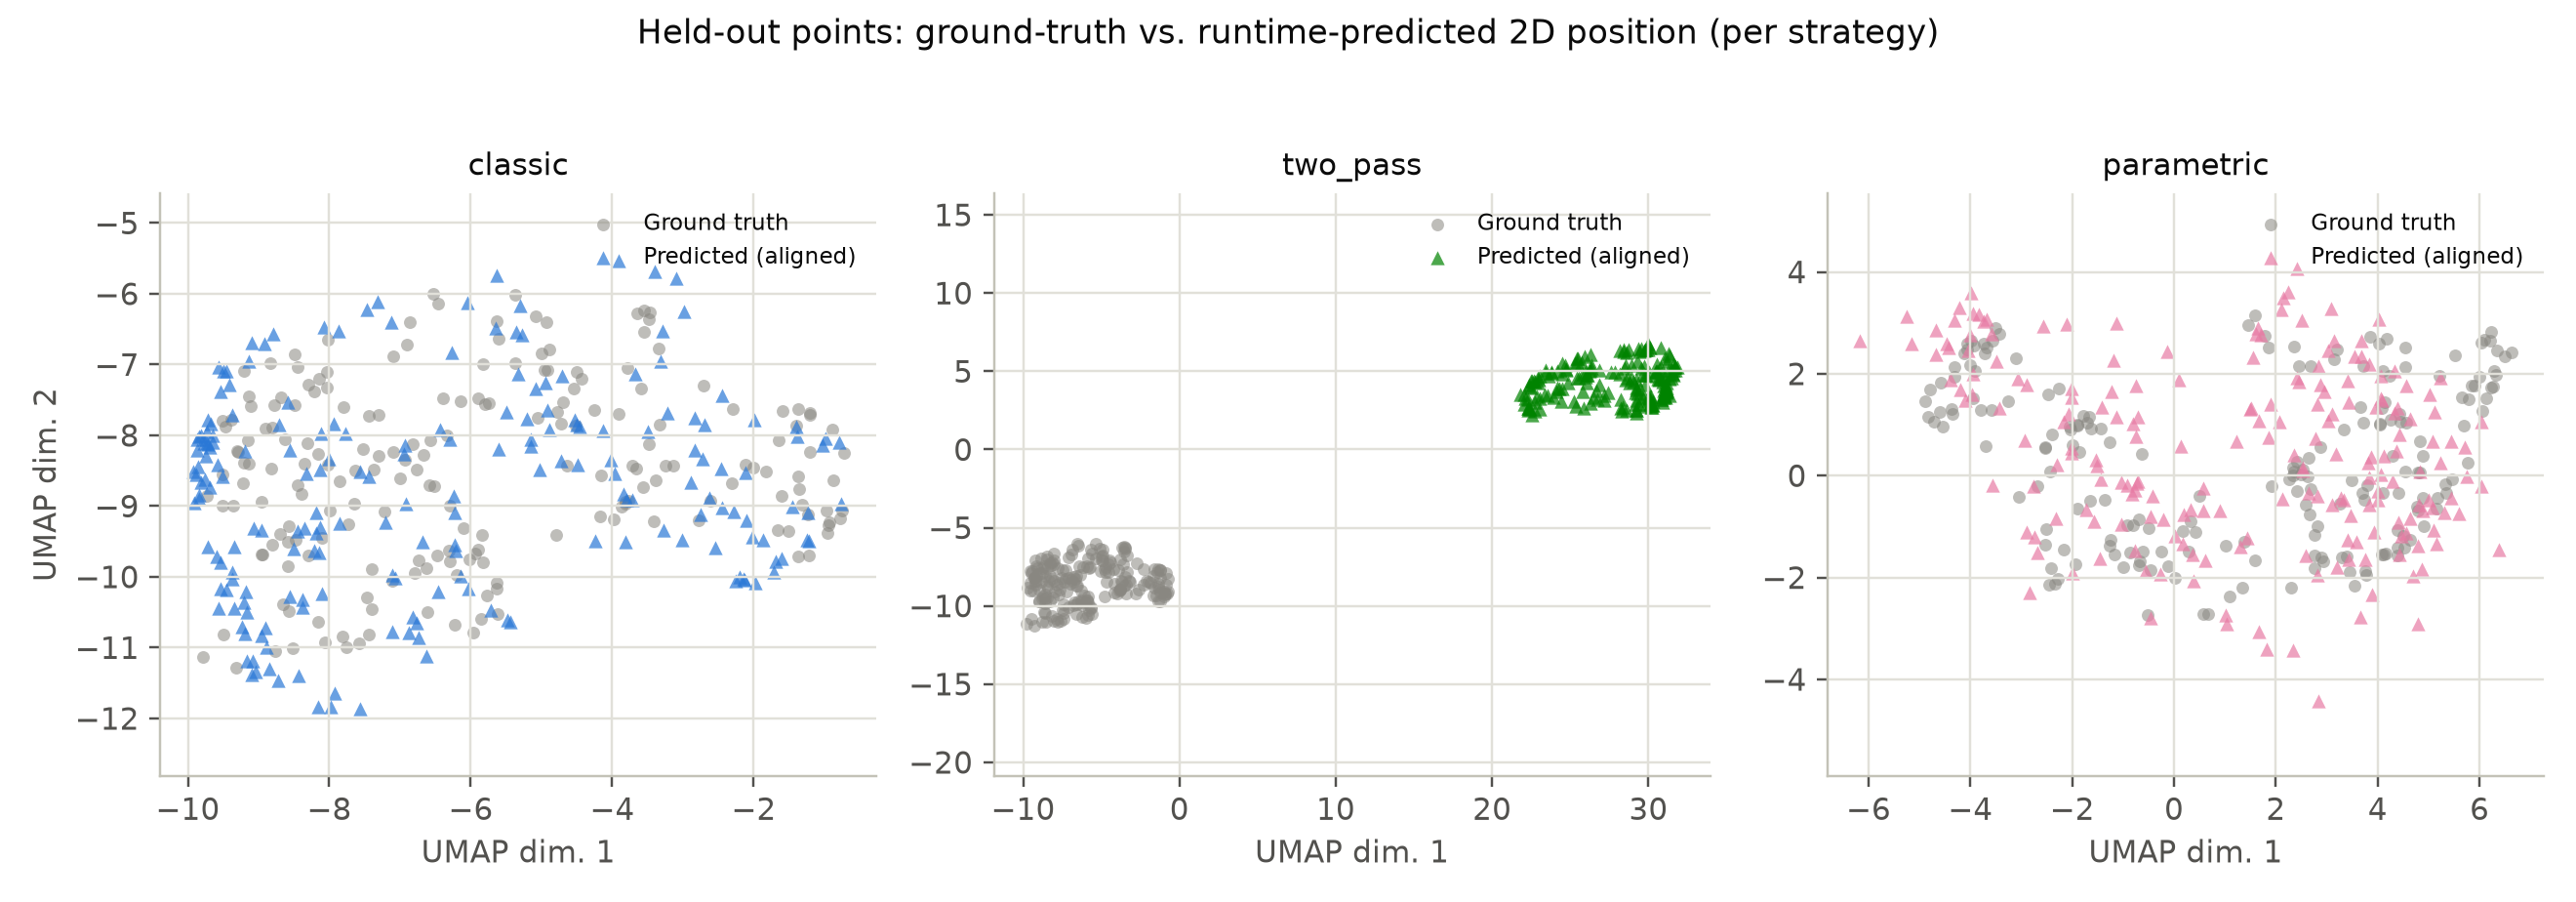
\includegraphics[width=0.9\textwidth]{figures/dataset-strategy-position-scatter.png}
\caption{Held-out points' ground-truth position (gray circles) against each strategy's Procrustes-aligned runtime-predicted position (colored triangles)}
\label{fig:dataset-strategy-position-scatter}
\end{figure}

\hyperref[fig:dataset-strategy-position-scatter]{Figure~\ref*{fig:dataset-strategy-position-scatter}} shows this gap directly: \texttt{classic}'s and \texttt{parametric}'s predicted points fall inside the same region as their ground truth, while \texttt{two\_pass}'s predicted cluster sits entirely apart from where the held-out points actually belong, consistent with its far larger coordinate error in \hyperref[tbl:held-out-accuracy]{Table~\ref*{tbl:held-out-accuracy}}.

\FloatBarrier
\section{Interpolation behavior: LERP vs SLERP}\label{sec:5.3}

\hyperref[sec:4.8]{Section~4.8} introduced LERP and SLERP as alternative methods for interpolating between the same pair of source prompts, while \hyperref[sec:2.6]{Section~2.6} noted that geometric smoothness does not necessarily translate into perceptually smooth image transitions. The present section therefore examines whether the selected interpolation method and its resulting trajectory provide meaningful information about the quality and semantic continuity of the generated images, or whether these properties are influenced more strongly by other factors. LERP and SLERP are compared under identical experimental conditions across prompt pairs representing different levels of source-prompt similarity. Their intermediate states and trajectories are evaluated quantitatively using LPIPS and embedding-based similarity measures, following the evaluation framework established in \hyperref[sec:3.3]{Section~3.3}.

Six prompt pairs were selected from the \texttt{gustavosta\_sd\_prompts\_v2\_two\_pass} dataset, which contains 61.746 prompts and is one of the four large-scale operation datasets generated for this thesis. Pair selection combined a deterministic, algorithmic candidate-generation step with a subsequent manual curation step. The candidate pool was first restricted to 3.647 non-noise prompts of 40 to 140 characters in length. Eight anchor prompts were then drawn from this pool using a fixed random seed, and for each anchor, cosine similarity between compact embeddings was used to determine three tiered candidate partners: the highest-, median-, and lowest-similarity match, yielding 24 candidate pairs in total. From these 24 candidates, two of the eight anchors were dropped manually as less illustrative examples, leaving six anchors. Each of the six remaining anchors then contributed exactly one of its three tiered candidates to the final selection, yielding six pairs, two for each similarity tier: high similarity (0.98-0.99), medium similarity (0.85-0.92), and low similarity (0.72-0.73). The low tier represents the lowest similarity range that could be identified reliably under this procedure. For all eight original anchors, the lowest-similarity partner resolved to the same single prompt, suggesting that this prompt occupies an unusually isolated position in the compact embedding space. The final pair selection is fixed and documented in \texttt{pair\_manifest.json}.

For controlled execution, a small companion dataset was created containing only the 11 distinct prompts involved in the comparison. One endpoint occurs in both low-similarity pairs, as mentioned before, because it was the only suitable low-similarity partner that could be identified reliably for both anchor prompts. The resulting dataset therefore contains 11 rather than 12 unique prompts.
Using a separate companion dataset does not affect the interpolation results, because both interpolation operations re-encode the original prompt texts to obtain the full conditioning tensors required for generation, as descibed in \hyperref[sec:4.8]{Section~4.8}.

For each pair, LERP and SLERP were executed using the same five interpolation values, (0, 0.25, 0.5, 0.75, 1). All runs used the generation configuration defined in \hyperref[sec:5.1]{Section~5.1}. The experiment comprises three similarity tiers, two prompt pairs per tier and two interpolation methods, resulting in 12 trajectories in total. Each tier contains four trajectories: two produced with LERP and two with SLERP. The generated images and the compact embedding associated with each interpolation step were stored using an implemented save node.

Perceptual change is measured with LPIPS, using the \texttt{lpips} package, between each pair of consecutive generated images. Higher LPIPS values indicate stronger visual changes, whereas lower values indicate greater perceptual similarity. In parallel, cosine similarity is calculated between the compact embeddings of consecutive interpolation steps. Higher cosine similarity indicates that neighboring representations remain more similar, while lower values indicate stronger divergence.

For each trajectory, both measures are summarized across its four consecutive transitions. The reported statistics include the mean LPIPS and mean cosine similarity, as well as the most abrupt transition. This transition is identified by the maximum LPIPS value and the minimum cosine similarity. Tier-level results are obtained by averaging the trajectory-level values across the two prompt pairs evaluated with the same interpolation method.

\begin{table}[htbp]
\centering
\caption{Mean, worst-step LPIPS, cosine similarity per similarity tier and operation, averaged over the two pairs per tier}
\label{tbl:interpolation-tier-summary}
\resizebox{\textwidth}{!}{%
\begin{tabular}{|l|l|c|c|c|c|}
\hline
\textbf{Tier} & \textbf{Operation} & \textbf{LPIPS mean} & \textbf{LPIPS worst-step mean} & \textbf{Cosine-sim. mean} & \textbf{Cosine-sim. worst-step mean} \\
\hline
high & lerp & 0.571 & 0.676 & 0.9991 & 0.9991 \\
\hline
high & slerp & 0.569 & 0.676 & 0.9991 & 0.9991 \\
\hline
medium & lerp & 0.607 & 0.676 & 0.9926 & 0.9919 \\
\hline
medium & slerp & 0.609 & 0.678 & 0.9926 & 0.9919 \\
\hline
low & lerp & 0.623 & 0.685 & 0.9834 & 0.9804 \\
\hline
low & slerp & 0.624 & 0.688 & 0.9834 & 0.9804 \\
\hline
\end{tabular}%
}
\end{table}

\begin{figure}[htbp]
\centering
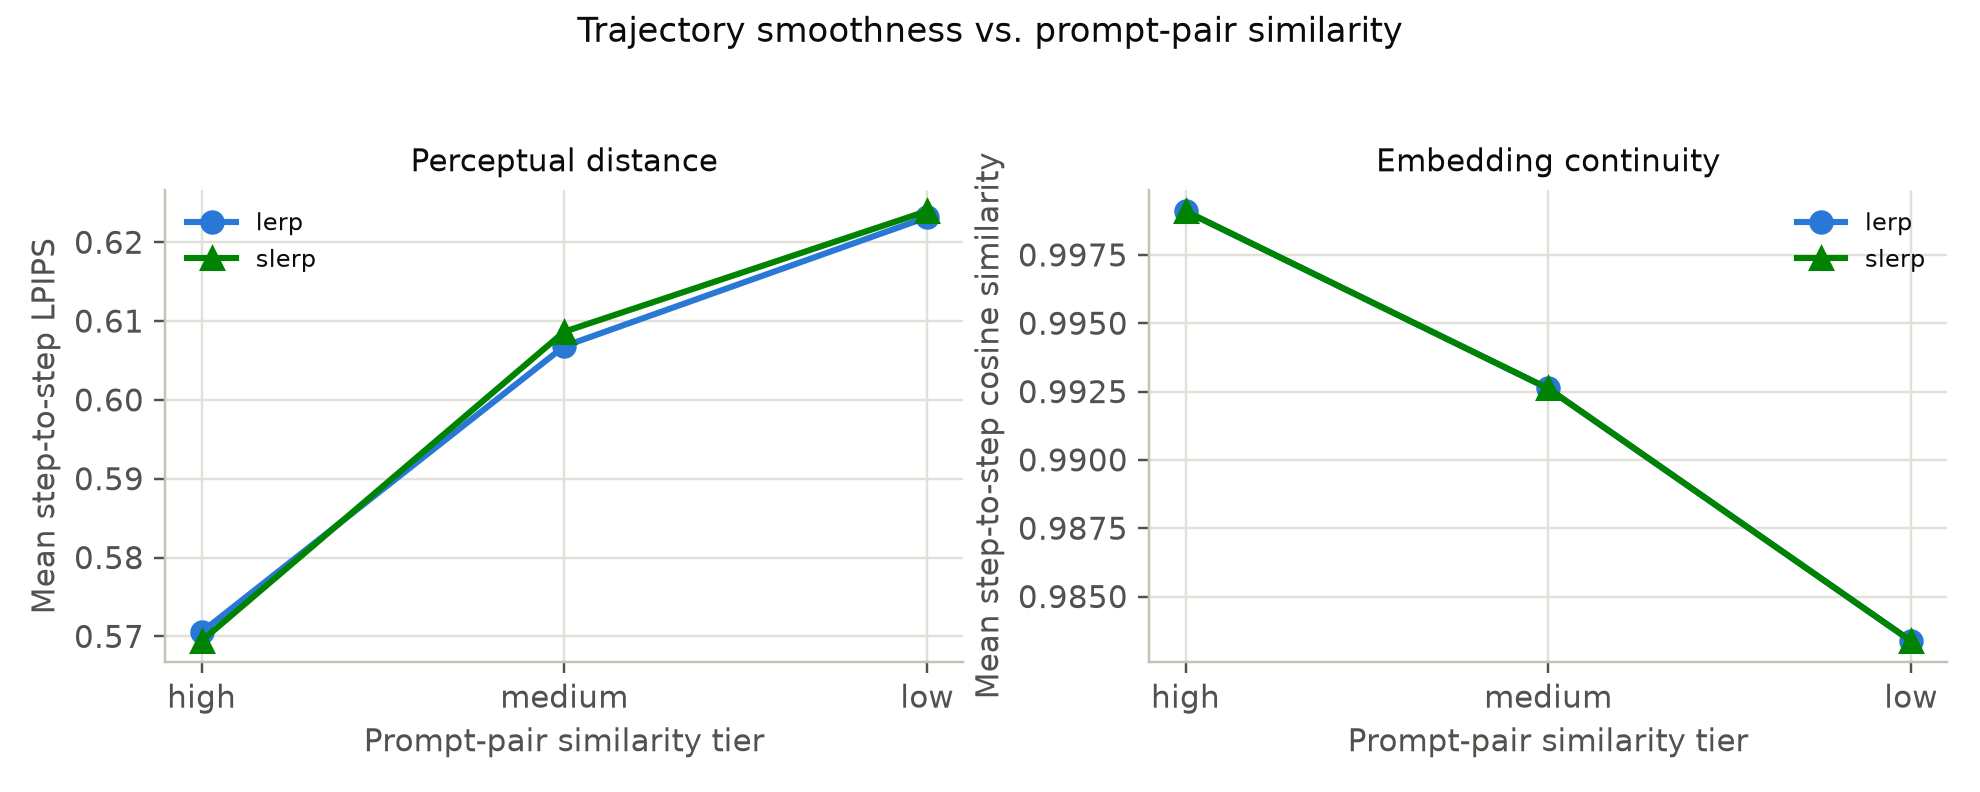
\includegraphics[width=0.9\textwidth]{figures/interpolation-tier-trend.png}
\caption{Mean step-to-step LPIPS and cosine similarity across the three similarity tiers}
\label{fig:interpolation-tier-trend}
\end{figure}

\hyperref[fig:interpolation-tier-trend]{Figure~\ref*{fig:interpolation-tier-trend}} and \hyperref[tbl:interpolation-tier-summary]{Table~\ref*{tbl:interpolation-tier-summary}} show the same overall pattern. From the high- to the low-similarity tier, mean LPIPS increases monotonically while mean cosine similarity decreases. This indicates that the similarity of the source prompts, rather than the interpolation method, is the primary factor determining how strongly consecutive trajectory steps differ. Within each tier, the results for LERP and SLERP differ only negligibly for both metrics, and neither method shows a consistent advantage in smoothness.

The largest individual transition within each trajectory shows a different pattern from the mean. Maximum step-wise LPIPS remains close to 0.68 across all three similarity tiers, whereas mean LPIPS rises from approximately 0.57 to 0.62. Thus, even trajectories between highly similar prompts contain at least one substantial perceptual change.

The location of this strongest LPIPS transition is also structured rather than random. In 8 of the 12 trajectories, it occurs between $\alpha=0.5$ and $\alpha=0.75$. In the remaining four trajectories, it occurs between $\alpha=0.25$ and $\alpha=0.5$. It never appears in either outer interval, and LERP and SLERP identify the same interval for each prompt pair, which is broadly consistent with the tier-averaged curves shown in \hyperref[fig:interpolation-step-profile]{Figure~\ref*{fig:interpolation-step-profile}} below. By contrast, the minimum step-wise cosine similarity occurs across all four intervals and does not exhibit a similarly consistent positional pattern.

\begin{figure}[htbp]
\centering
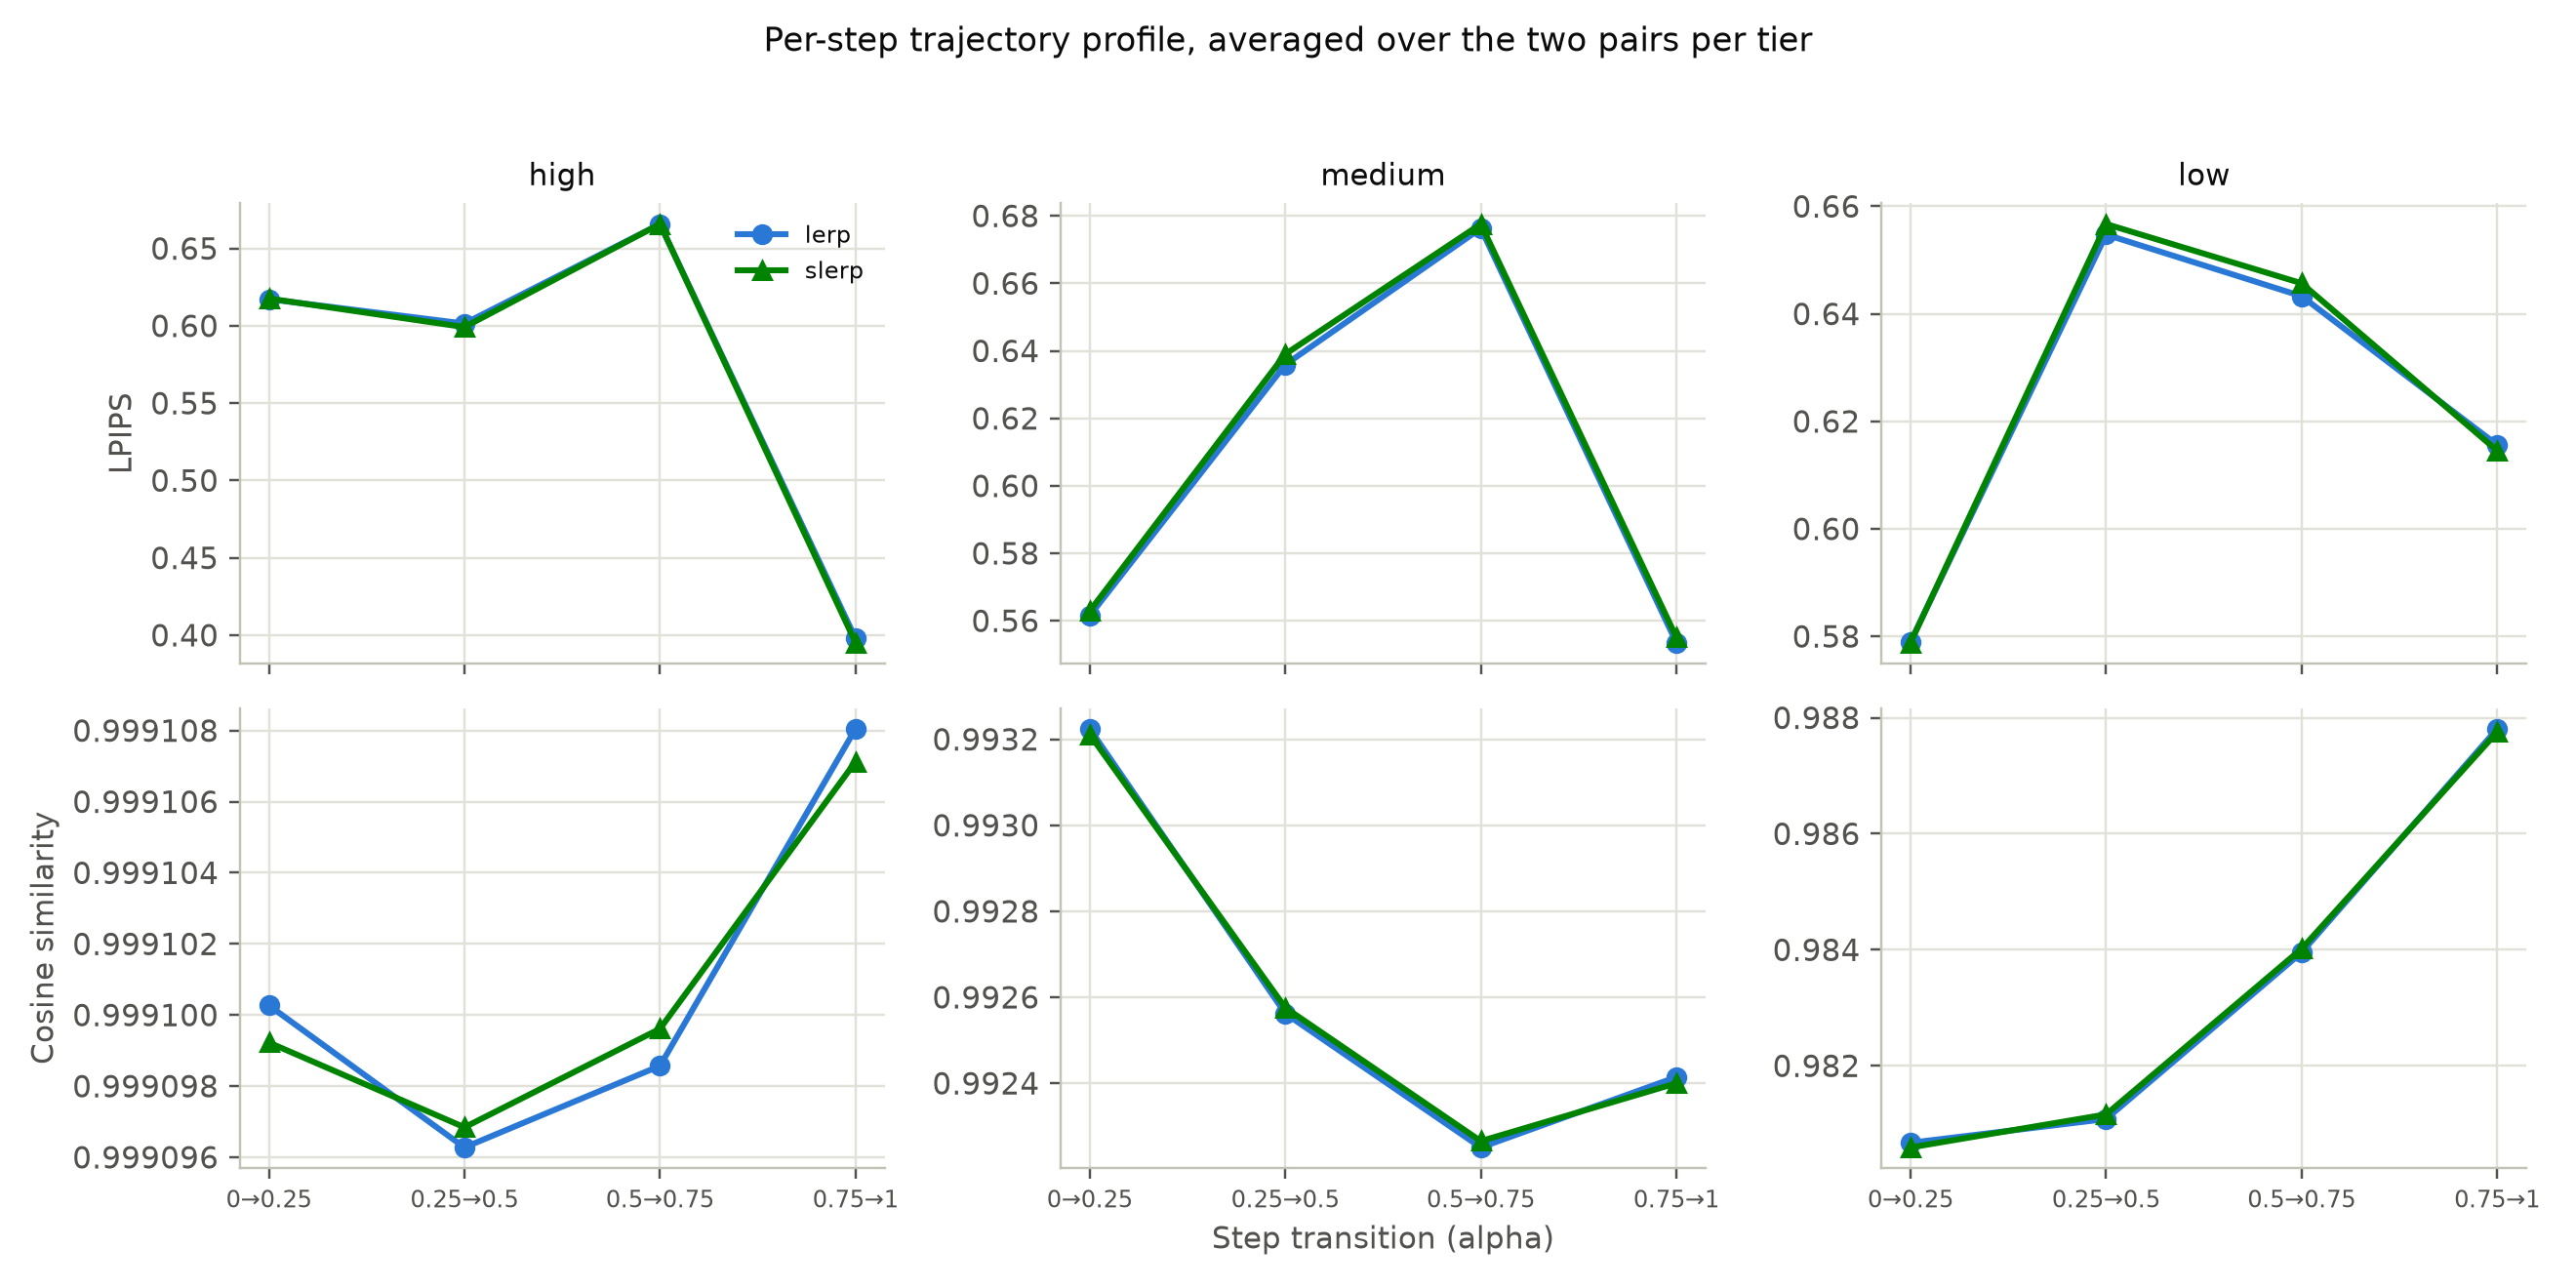
\includegraphics[width=0.9\textwidth]{figures/interpolation-step-profile.png}
\caption{Per-step LPIPS and cosine similarity profile across the four step transitions, averaged over the two pairs per tier}
\label{fig:interpolation-step-profile}
\end{figure}

A structured qualitative review examined both endpoints and the transition with the highest LPIPS value for all 12 trajectories. In every case, the images generated at ($\alpha=0$) and ($\alpha=1$) were clearly consistent with their respective endpoint prompts, and no visible artifacts or incoherent outputs were observed at any interpolation step. The largest LPIPS changes generally corresponded to substantial shifts in scene or subject matter rather than to a decline in image quality. For example, pair 4 transitions from a bear-like monster to a nurse portrait at ($\alpha=0.75$) (\hyperref[fig:interpolation-strip-medium]{Figure~\ref*{fig:interpolation-strip-medium}}). Pair 5, the least similar pair in the experiment, produced the most distinctive intermediate result: at ($\alpha=0.75$), the generated image depicts a spacecraft arriving above a medieval settlement, forming a coherent combination of both endpoint concepts rather than an abrupt transition between them (\hyperref[fig:interpolation-strip-low]{Figure~\ref*{fig:interpolation-strip-low}}).

\begin{figure}[htbp]
\centering
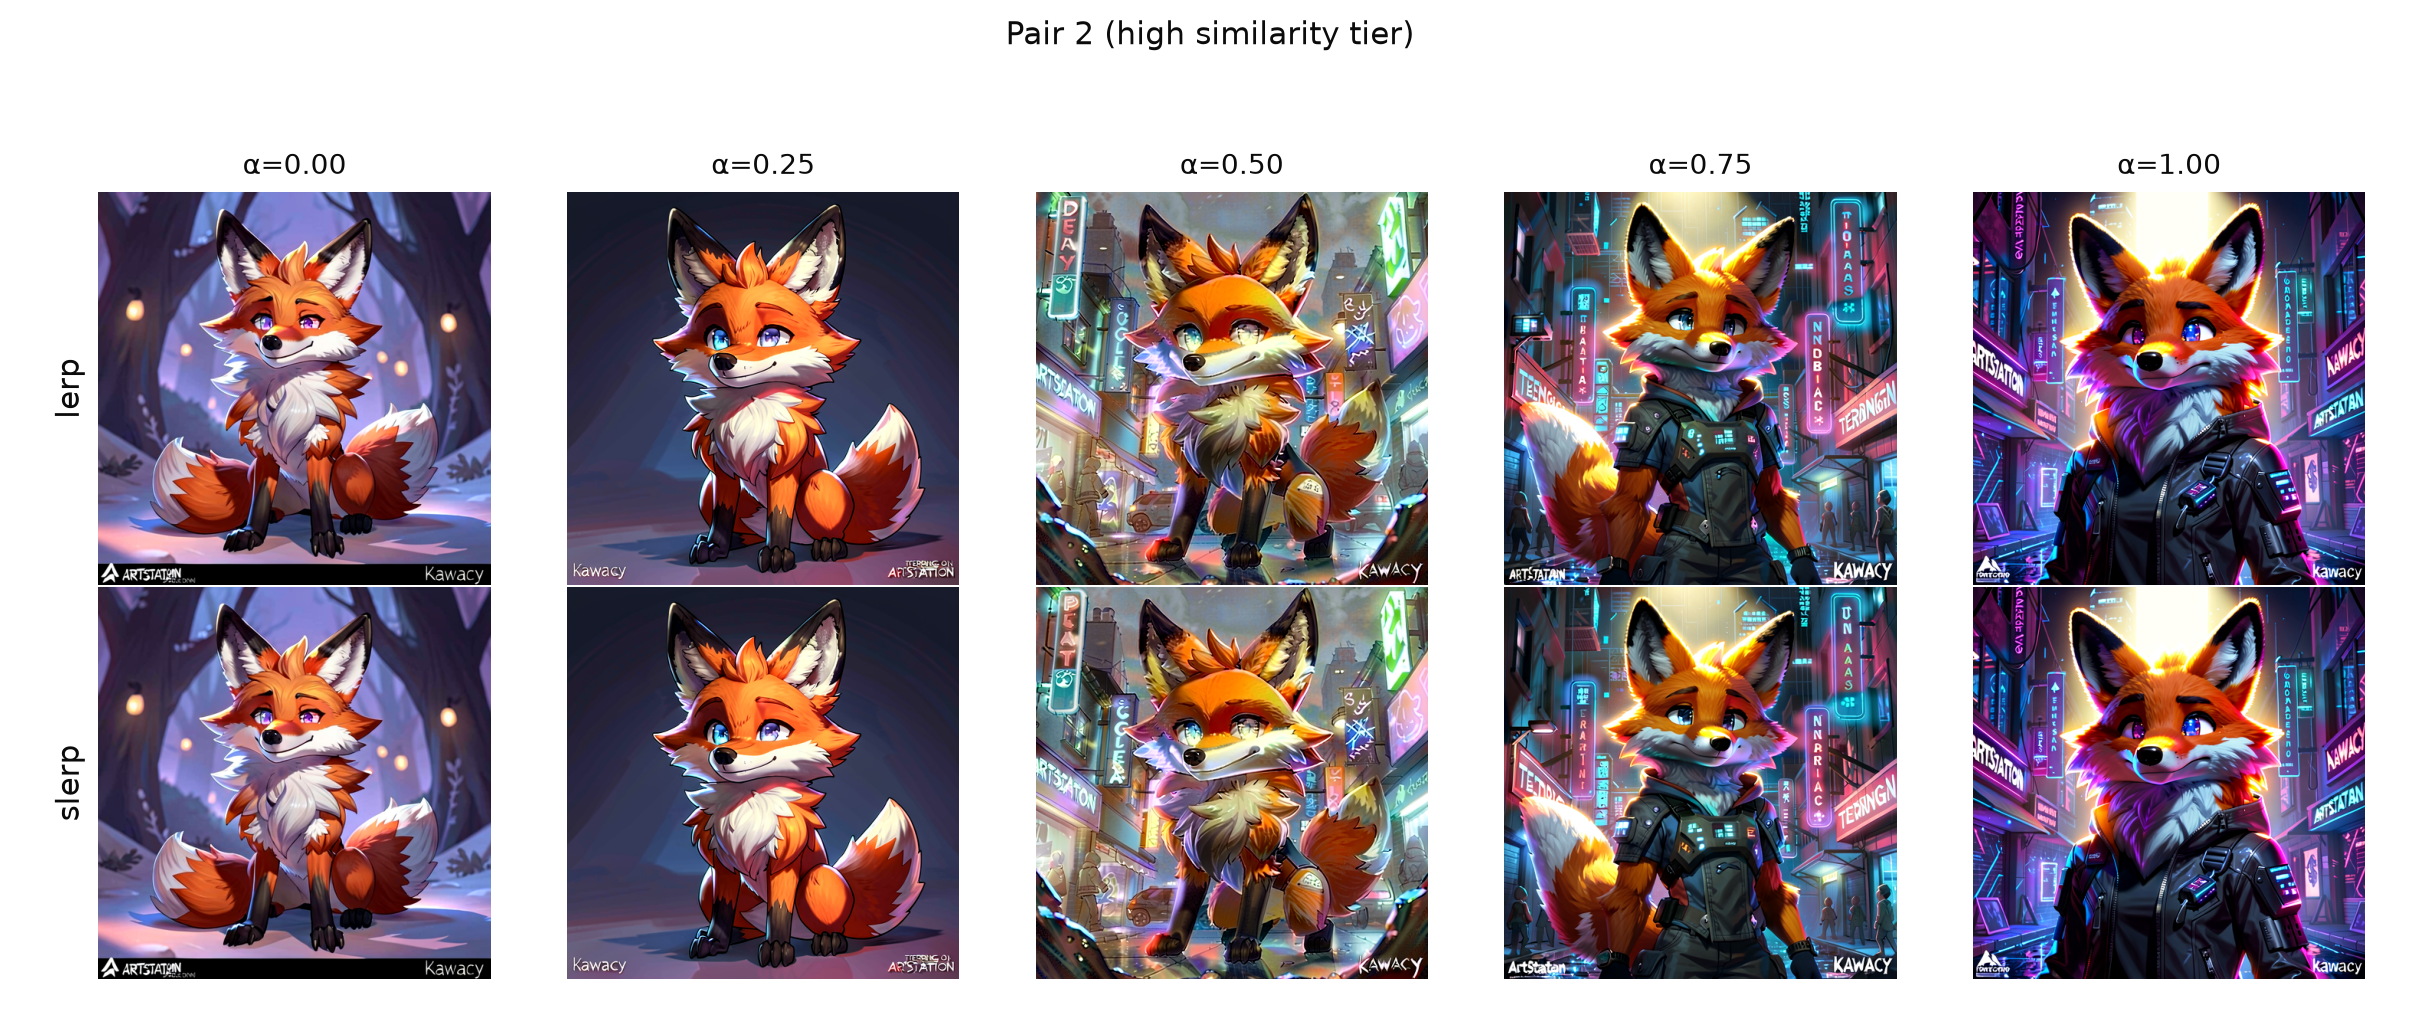
\includegraphics[width=\textwidth]{figures/interpolation-strip-high.png}
\caption[Representative trajectory, high-similarity tier (pair 2): forest fox to cyberpunk-styled fox]{Representative trajectory, high-similarity tier (pair 2): forest fox to cyberpunk-styled fox. A: "a fox fursona, trending on artstation, by kawacy, furry art, digital art". B: "a fox fursona, trending on artstation, by kawacy, furry art, digital art, cyberpunk, high quality, backlighting"}
\label{fig:interpolation-strip-high}
\end{figure}

\begin{figure}[htbp]
\centering
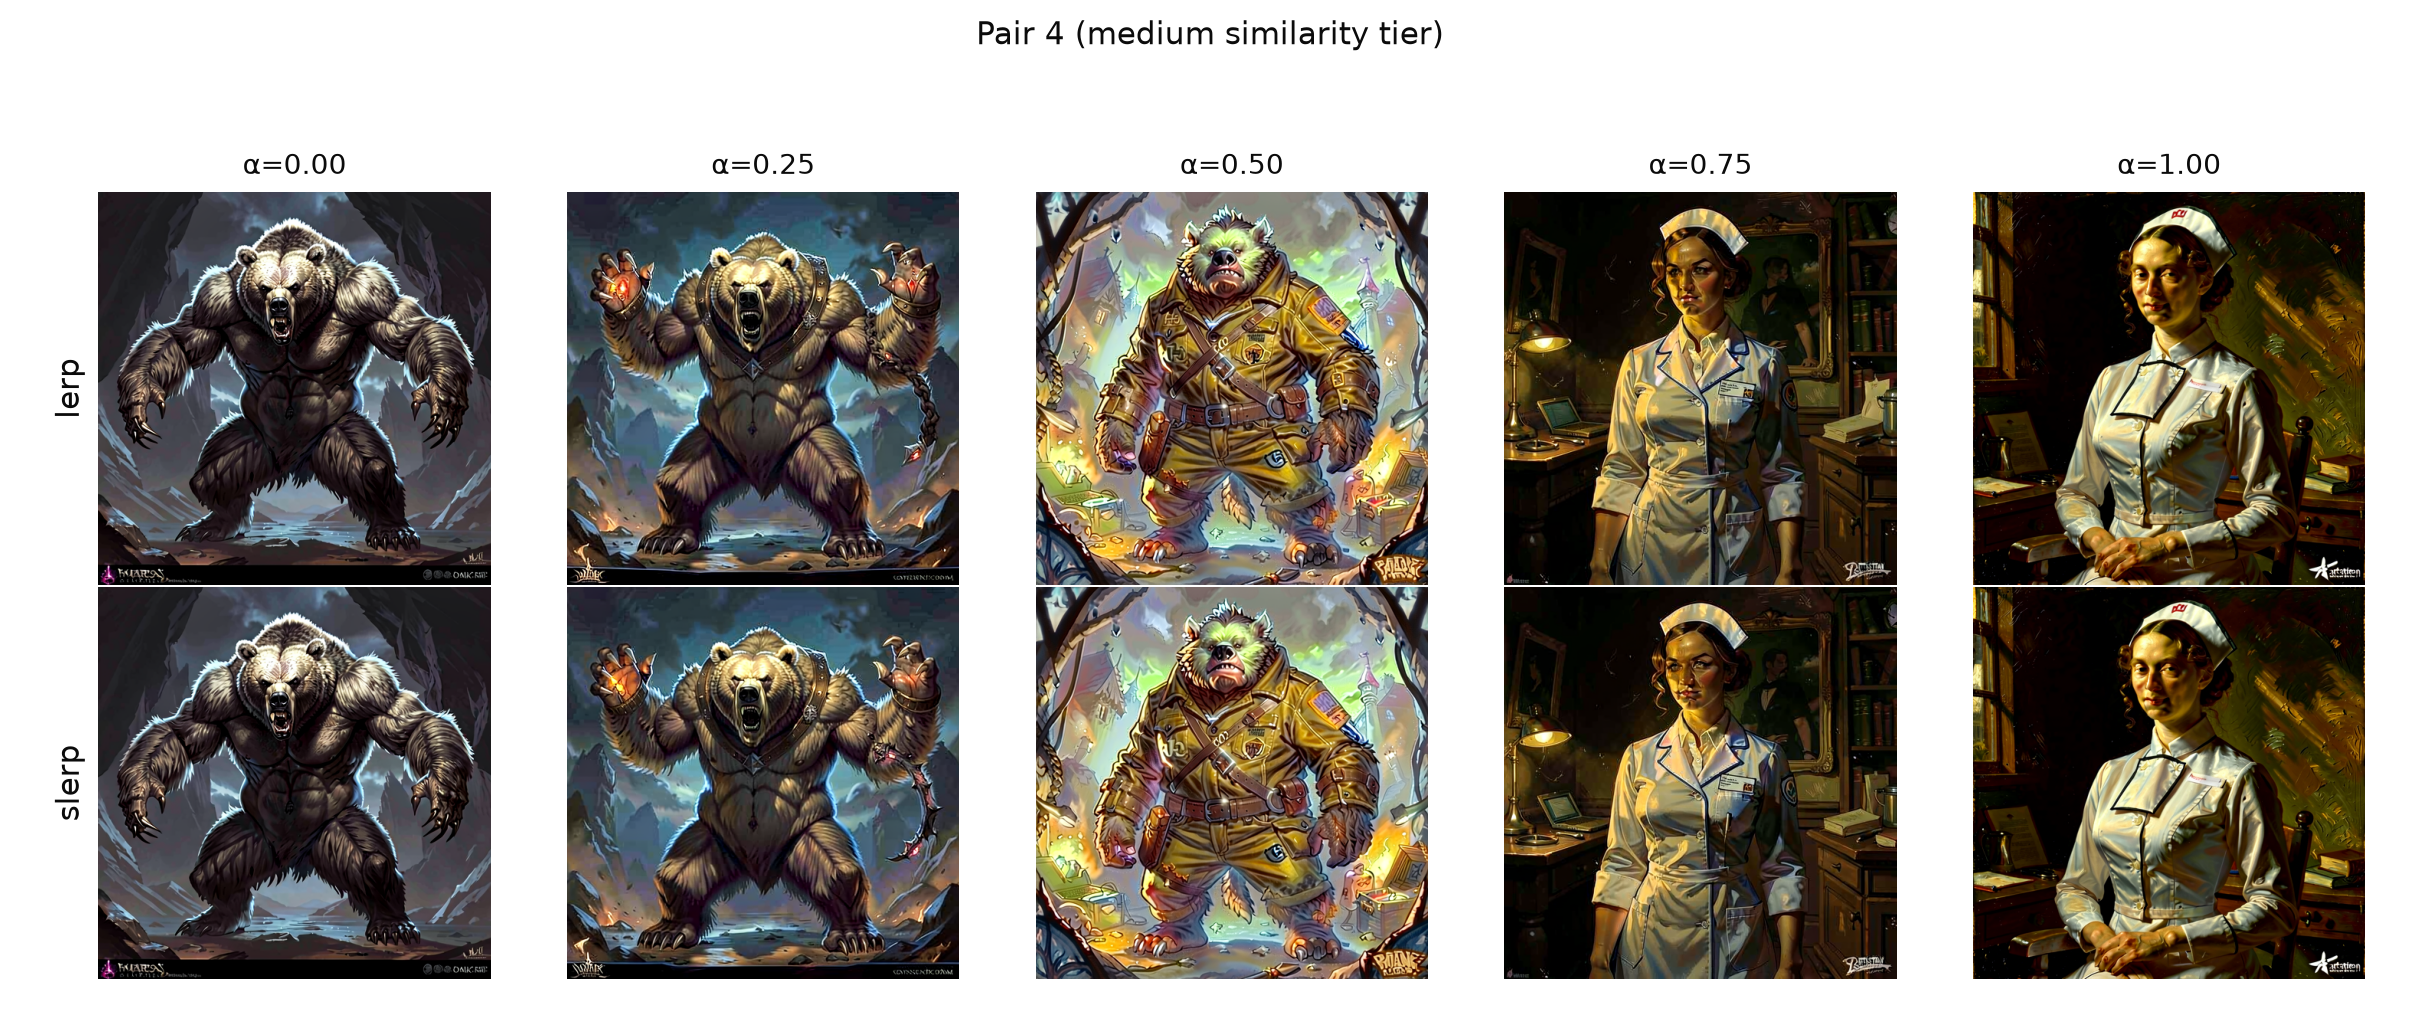
\includegraphics[width=\textwidth]{figures/interpolation-strip-medium.png}
\caption[Representative trajectory, medium-similarity tier (pair 4): grizzly bear monster to nurse portrait]{Representative trajectory, medium-similarity tier (pair 4): grizzly bear monster to nurse portrait. A: "a ferocious grizzly bear monster with 4 arms, fantasy concept art, detailed, epic pose". B: "Female in nurse suit. By Rembrandt and artstation trending"}
\label{fig:interpolation-strip-medium}
\end{figure}

\begin{figure}[htbp]
\centering
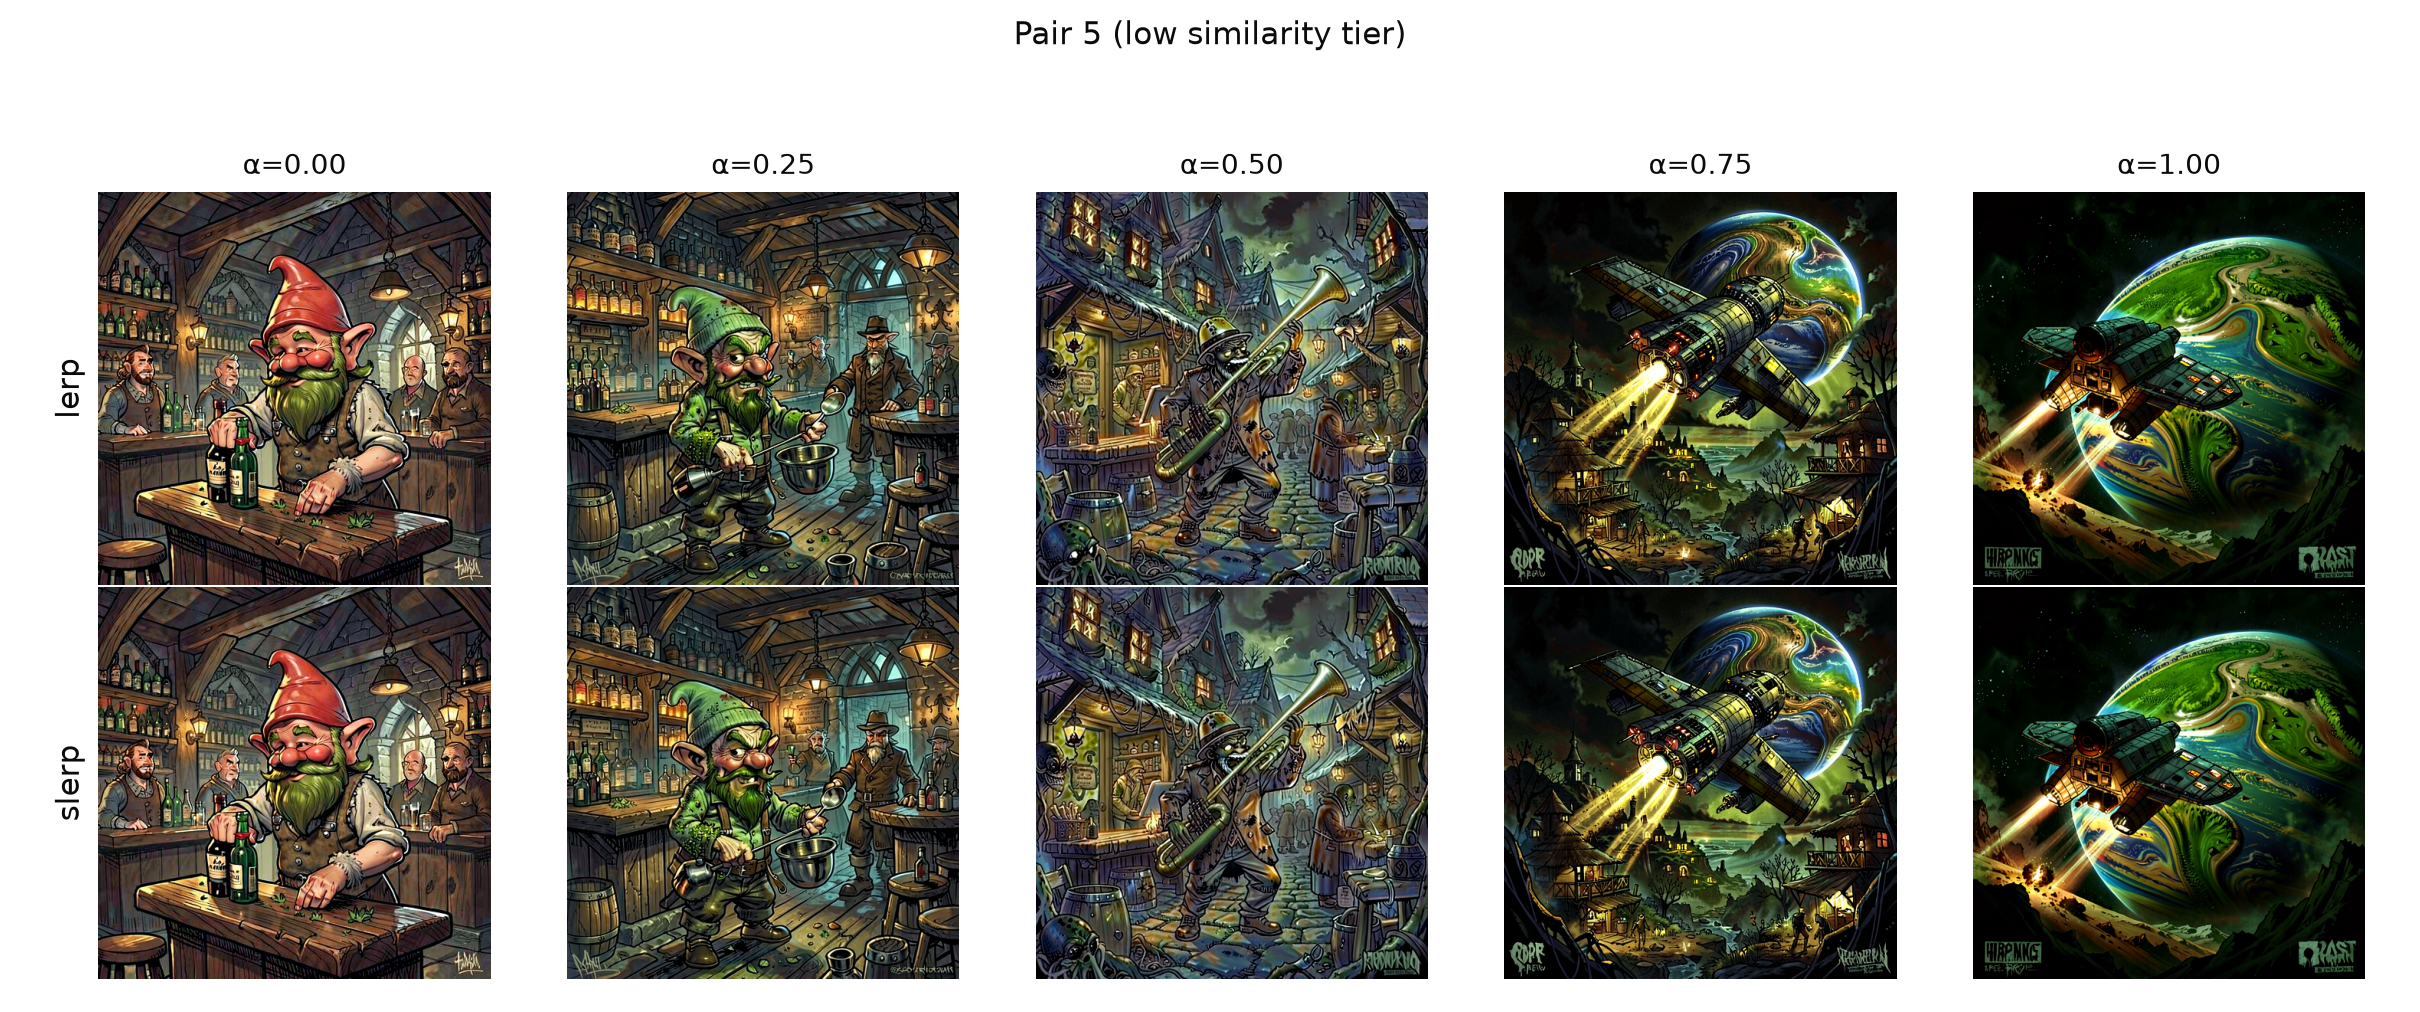
\includegraphics[width=\textwidth]{figures/interpolation-strip-low.png}
\caption[Representative trajectory, low-similarity tier (pair 5): garden gnome in a medieval tavern to spacecraft]{Representative trajectory, low-similarity tier (pair 5): garden gnome in a medieval tavern to spacecraft, including the fusion result at $\alpha=0.75$. A: "garden gnome bartending in a medieval tavern, concept art, john howe". B: "concept art of spacecraft arriving at the last habitable planet, shot from a horror film"}
\label{fig:interpolation-strip-low}
\end{figure}

Finally, three representative trajectories were projected into the embedding space of \texttt{gustavosta\_sd\_prompts\_v2\_two\_pass}. Rather than using the UMAP model fitted on the 11-prompt companion dataset, the analysis employed the large dataset's \texttt{two\_pass} runtime reducer. Since this reducer was trained on a 20,000-point subset of the original dataset, it provides a more representative reference space for positioning the trajectory embeddings. The five saved compact embeddings from each trajectory were transformed using this reducer and plotted against the dataset's own canonical positions for context. The 2D figure shows all 61.746 points, while the 3D figure, zoomed into each trajectory's own local neighborhood.

\begin{figure}[htbp]
\centering
\begin{subfigure}[b]{\textwidth}
\centering
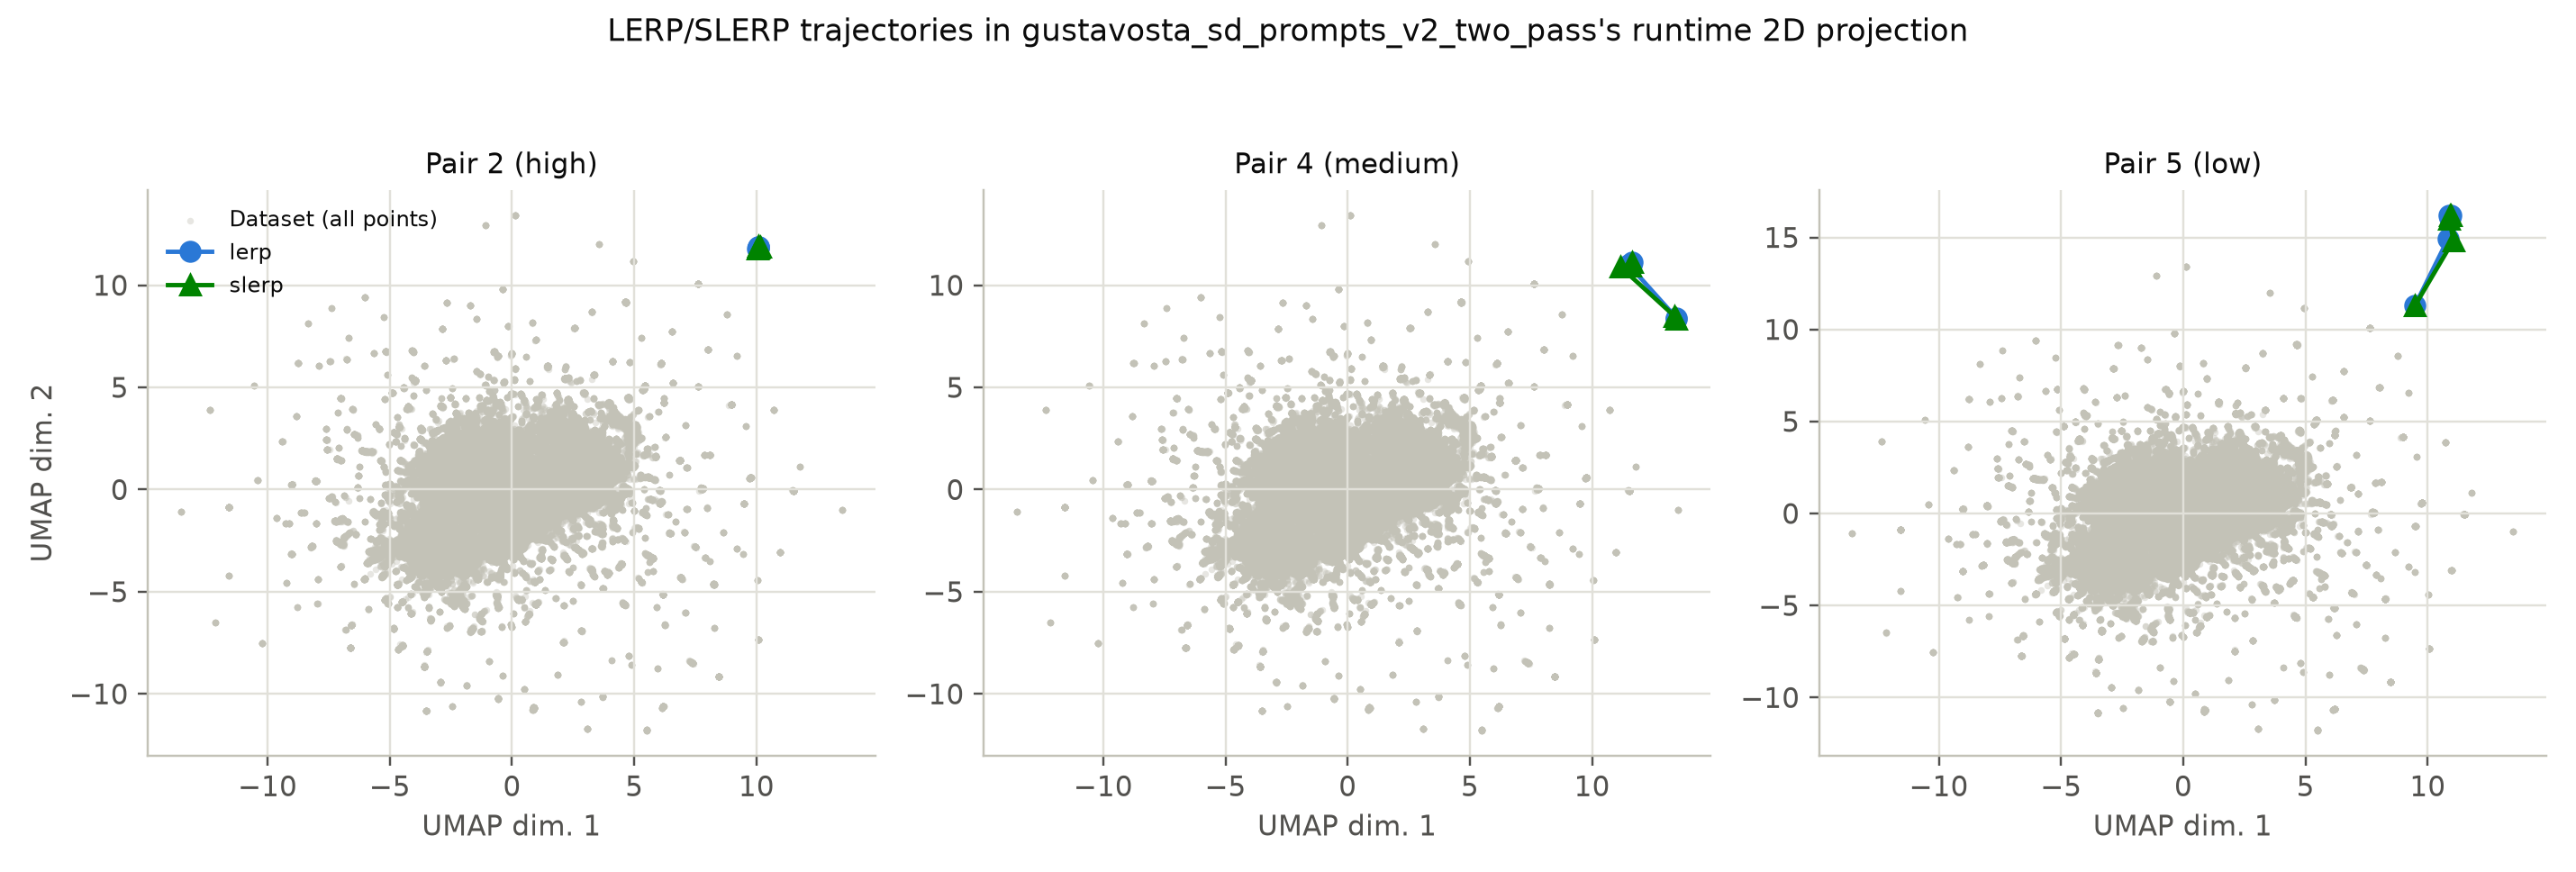
\includegraphics[width=0.9\textwidth]{figures/interpolation-trajectory-graph-2d.png}
\caption{Projected through the dataset's runtime 2D reducer, against all 61.746 dataset points}
\label{fig:interpolation-trajectory-graph-2d}
\end{subfigure}
\begin{subfigure}[b]{\textwidth}
\centering
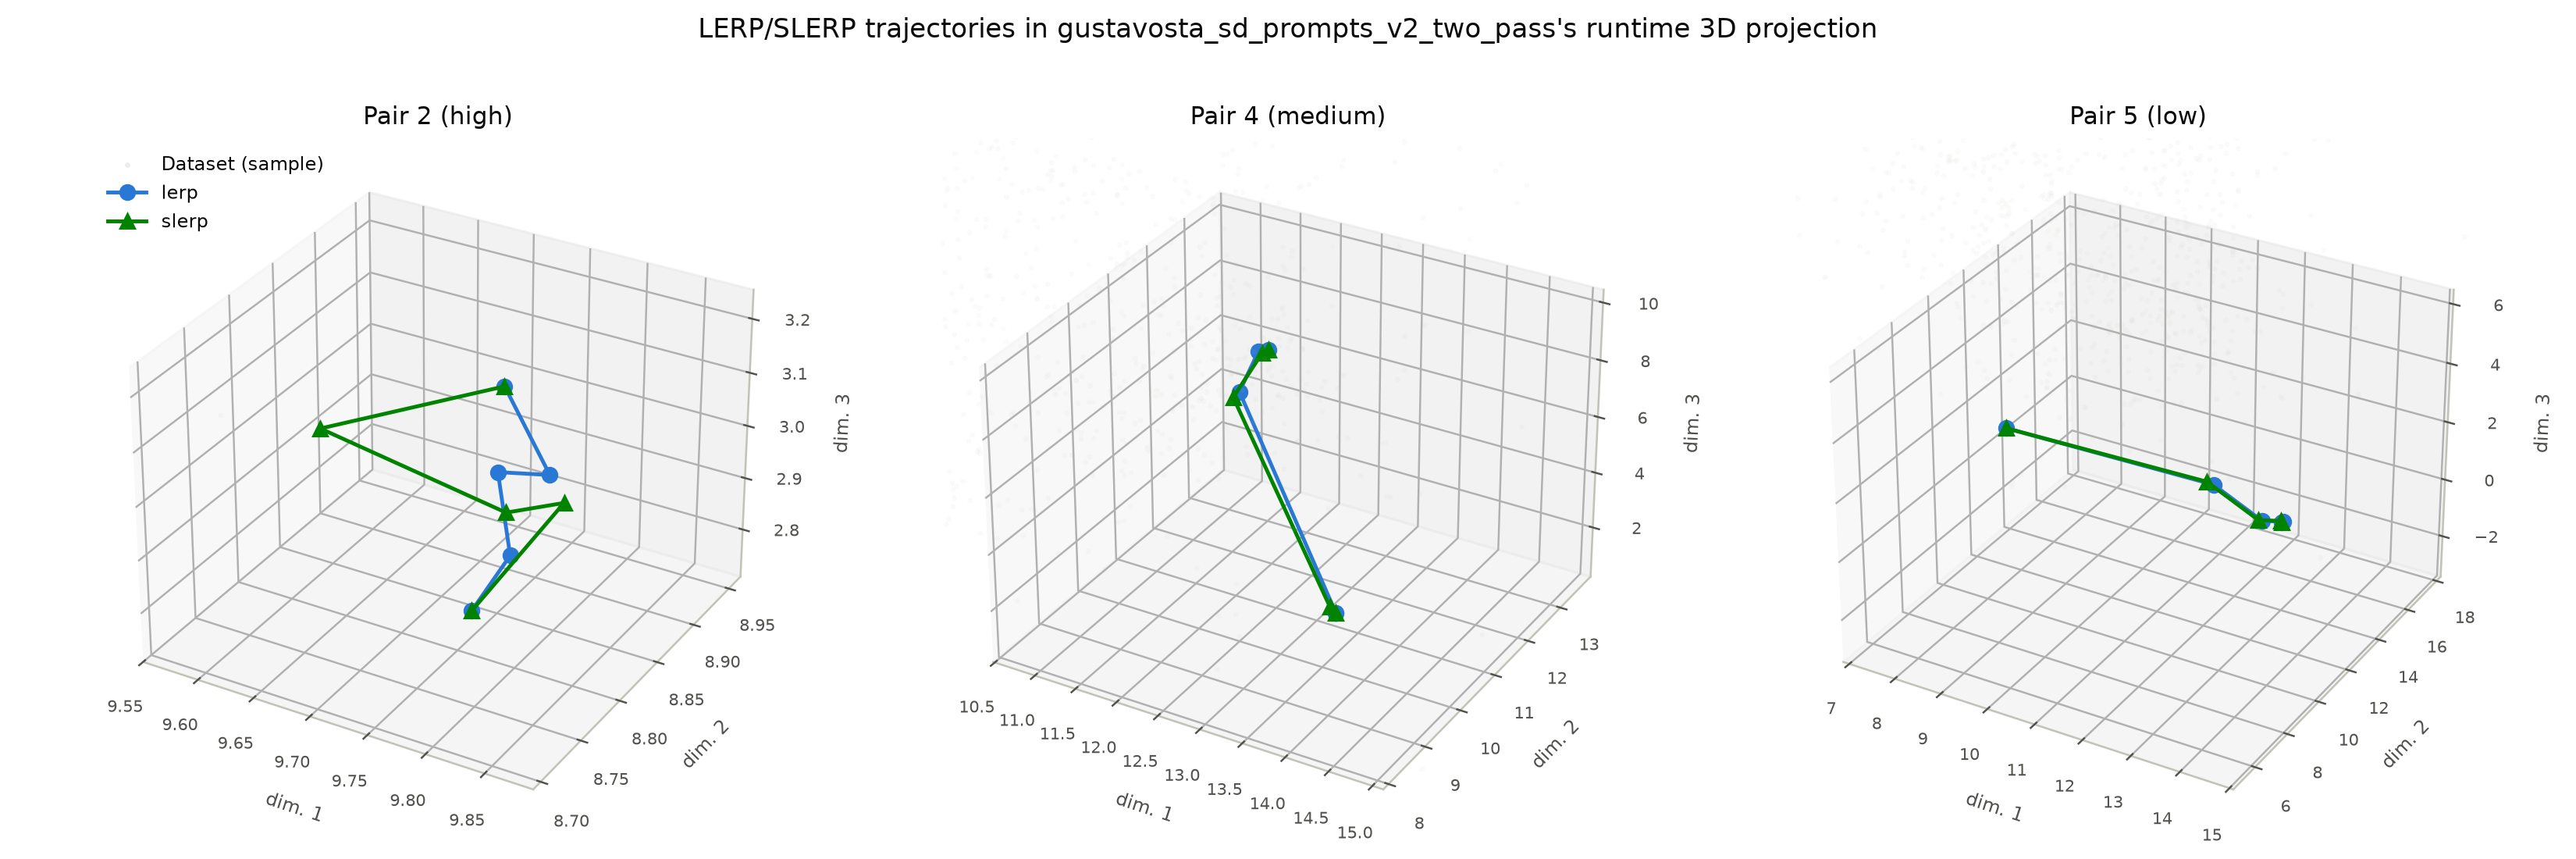
\includegraphics[width=0.9\textwidth]{figures/interpolation-trajectory-graph-3d.png}
\caption{The same three trajectories in the runtime 3D reducer's output, axis limits zoomed to each trajectory's own neighborhood rather than the full sample}
\label{fig:interpolation-trajectory-graph-3d}
\end{subfigure}
\caption{LERP/SLERP trajectories of three representative pairs, in the runtime 2D and 3D reducer output}
\label{fig:interpolation-trajectory-graph}
\end{figure}

\hyperref[fig:interpolation-trajectory-graph-2d]{Figure~\ref*{fig:interpolation-trajectory-graph-2d}} shows that all three trajectories lie near the boundary of, or outside, the main density region of the full dataset. This is consistent with the finding in \hyperref[sec:5.2]{Section~5.2} that the \texttt{two\_pass} runtime reducer provides a comparatively weak approximation for genuinely unseen points. The trajectory steps represent an even more pronounced out-of-sample case than the held-out prompts evaluated there, since they are derived from newly generated intermediate states rather than from prompts contained in the original corpus. Their position should therefore be interpreted primarily as a limitation of the runtime reducer's generalization rather than as reliable evidence of where these states belong in the underlying compact embedding space.

The projected trajectories also do not always move consistently between their endpoints, although LERP and SLERP follow simple, well-defined paths in the original conditioning space. This is not necessarily contradictory, since UMAP is designed to preserve local neighborhood relationships rather than global distances or straight-line geometry. A linear trajectory in a high-dimensional space is therefore not guaranteed to remain straight or monotonic after dimensionality reduction.
In the three-dimensional view shown in \hyperref[fig:interpolation-trajectory-graph-3d]{Figure~\ref*{fig:interpolation-trajectory-graph-3d}}, pair 2's paths separate visibly at the intermediate steps once the third dimension is included, despite its generated images (\hyperref[fig:interpolation-strip-high]{Figure~\ref*{fig:interpolation-strip-high}}) and two-dimensional trajectories being nearly indistinguishable between LERP and SLERP. By contrast, the LERP and SLERP trajectories for pairs 4 and 5 remain close to a common path in all three dimensions. This shows that lower-dimensional projections can hide structures that become visible only when additional dimensions are considered. However, the present results do not establish whether the observed trajectories represent genuine local structure preserved by the reducer or instead result from its limited accuracy when projecting unseen points.

Within this experiment, source-prompt similarity was the main factor determining the magnitude of change between consecutive trajectory steps. By comparison, the choice between LERP and SLERP had only a minor effect on both perceptual and embedding-based measures, with both methods producing visually and quantitatively similar generated images across all three similarity tiers, despite their trajectories sometimes taking visibly different paths through the projected embedding space.

These results do not establish that interpolation geometry is generally irrelevant to image generation. They show only that no meaningful difference between LERP and SLERP could be detected under the conditions examined here. The findings also place SLERP's usual theoretical motivation in context: although SLERP is generally motivated by better-preserved vector norms compared to LERP's straight-line blend, this theoretical advantage did not translate into measurably or perceptually smoother trajectories in the evaluated system and at the tested scale.

\FloatBarrier
\section{Direction transfer with Delta / Direction Walk}\label{sec:5.4}

\hyperref[sec:4.8]{Section~4.8} introduced Direction Walk as the transfer of a direction defined by two anchor prompts to an independent starting point. Unlike interpolation, the operation is not restricted to the interval between the anchors. Values of $\alpha$ may extend across $[-2, 4]$, allowing the direction to be applied in reverse or extrapolated beyond a complete transfer. The present section evaluates whether such a direction produces a meaningful and consistent transformation when applied to unrelated starting contexts across this extended range.

Three directions were selected for the experiment. Each was applied to two independent starting prompts $C$. The first represented a near context with clear conceptual overlap with the anchor prompts $A$ and $B$. The second represented a far context without an obvious shared subject. All source prompts originate from \texttt{gustavosta\_sd\_prompts\_v2\_two\_pass} and were loaded through a small companion dataset constructed in the same manner as in the previous section.

Each of the six walks was evaluated using the same sequence of direction strengths: -2, -1, 0, 1, 2, 3, 4. All runs used the shared generation configuration defined at the beginning of this chapter. Each walk therefore produced seven generated images and seven corresponding compact embeddings. The step at $\alpha=0$ represents the unmodified starting prompt $C$.

Two complementary forms of comparison were calculated from the saved images and embeddings, using the LPIPS and cosine-similarity measures introduced earlier. Consecutive-step comparisons evaluate each point against its immediate predecessor and therefore describe local continuity along the walk. Baseline-relative comparisons instead evaluate every step against the unmodified starting state at $\alpha=0$. They measure how strongly the result departs from its original context as the direction strength increases. This second perspective is particularly relevant for Direction Walk because it directly tests whether a direction derived from one prompt pair induces a systematic transformation when transferred to a different starting context.

\begin{table}[htbp]
\centering
\caption[Consecutive-step and baseline-relative summary per direction and starting context]{Consecutive-step and baseline-relative summary per direction and starting context. Baseline values report the single largest drift from the $\alpha=0$ step (LPIPS) or the single closest departure from it (cosine similarity), together with the alpha at which it occurred}
\label{tbl:delta-walk-summary}
\resizebox{\textwidth}{!}{%
\begin{tabular}{|l|l|c|c|c|c|}
\hline
\textbf{Direction} & \textbf{Context} & \textbf{Consec. LPIPS mean} & \textbf{Consec. LPIPS max} & \textbf{Baseline LPIPS max ($\alpha$)} & \textbf{Baseline cosine-sim. min ($\alpha$)} \\
\hline
1 (cyberpunk styling) & near & 0.636 & 0.797 & 0.820 ($\alpha$=3) & 0.756 ($\alpha$=4) \\
\hline
1 (cyberpunk styling) & far & 0.574 & 0.597 & 0.606 ($\alpha$=4) & 0.837 ($\alpha$=4) \\
\hline
2 (shoes $\to$ jacket) & near & 0.565 & 0.707 & 0.846 ($\alpha$=-2) & 0.895 ($\alpha$=4) \\
\hline
2 (shoes $\to$ jacket) & far & 0.543 & 0.642 & 0.710 ($\alpha$=2) & 0.919 ($\alpha$=4) \\
\hline
3 (identity swap) & near & 0.579 & 0.643 & 0.664 ($\alpha$=4) & 0.746 ($\alpha$=4) \\
\hline
3 (identity swap) & far & 0.647 & 0.696 & 0.790 ($\alpha$=3) & 0.748 ($\alpha$=4) \\
\hline
\end{tabular}%
}
\end{table}

\begin{figure}[htbp]
\centering
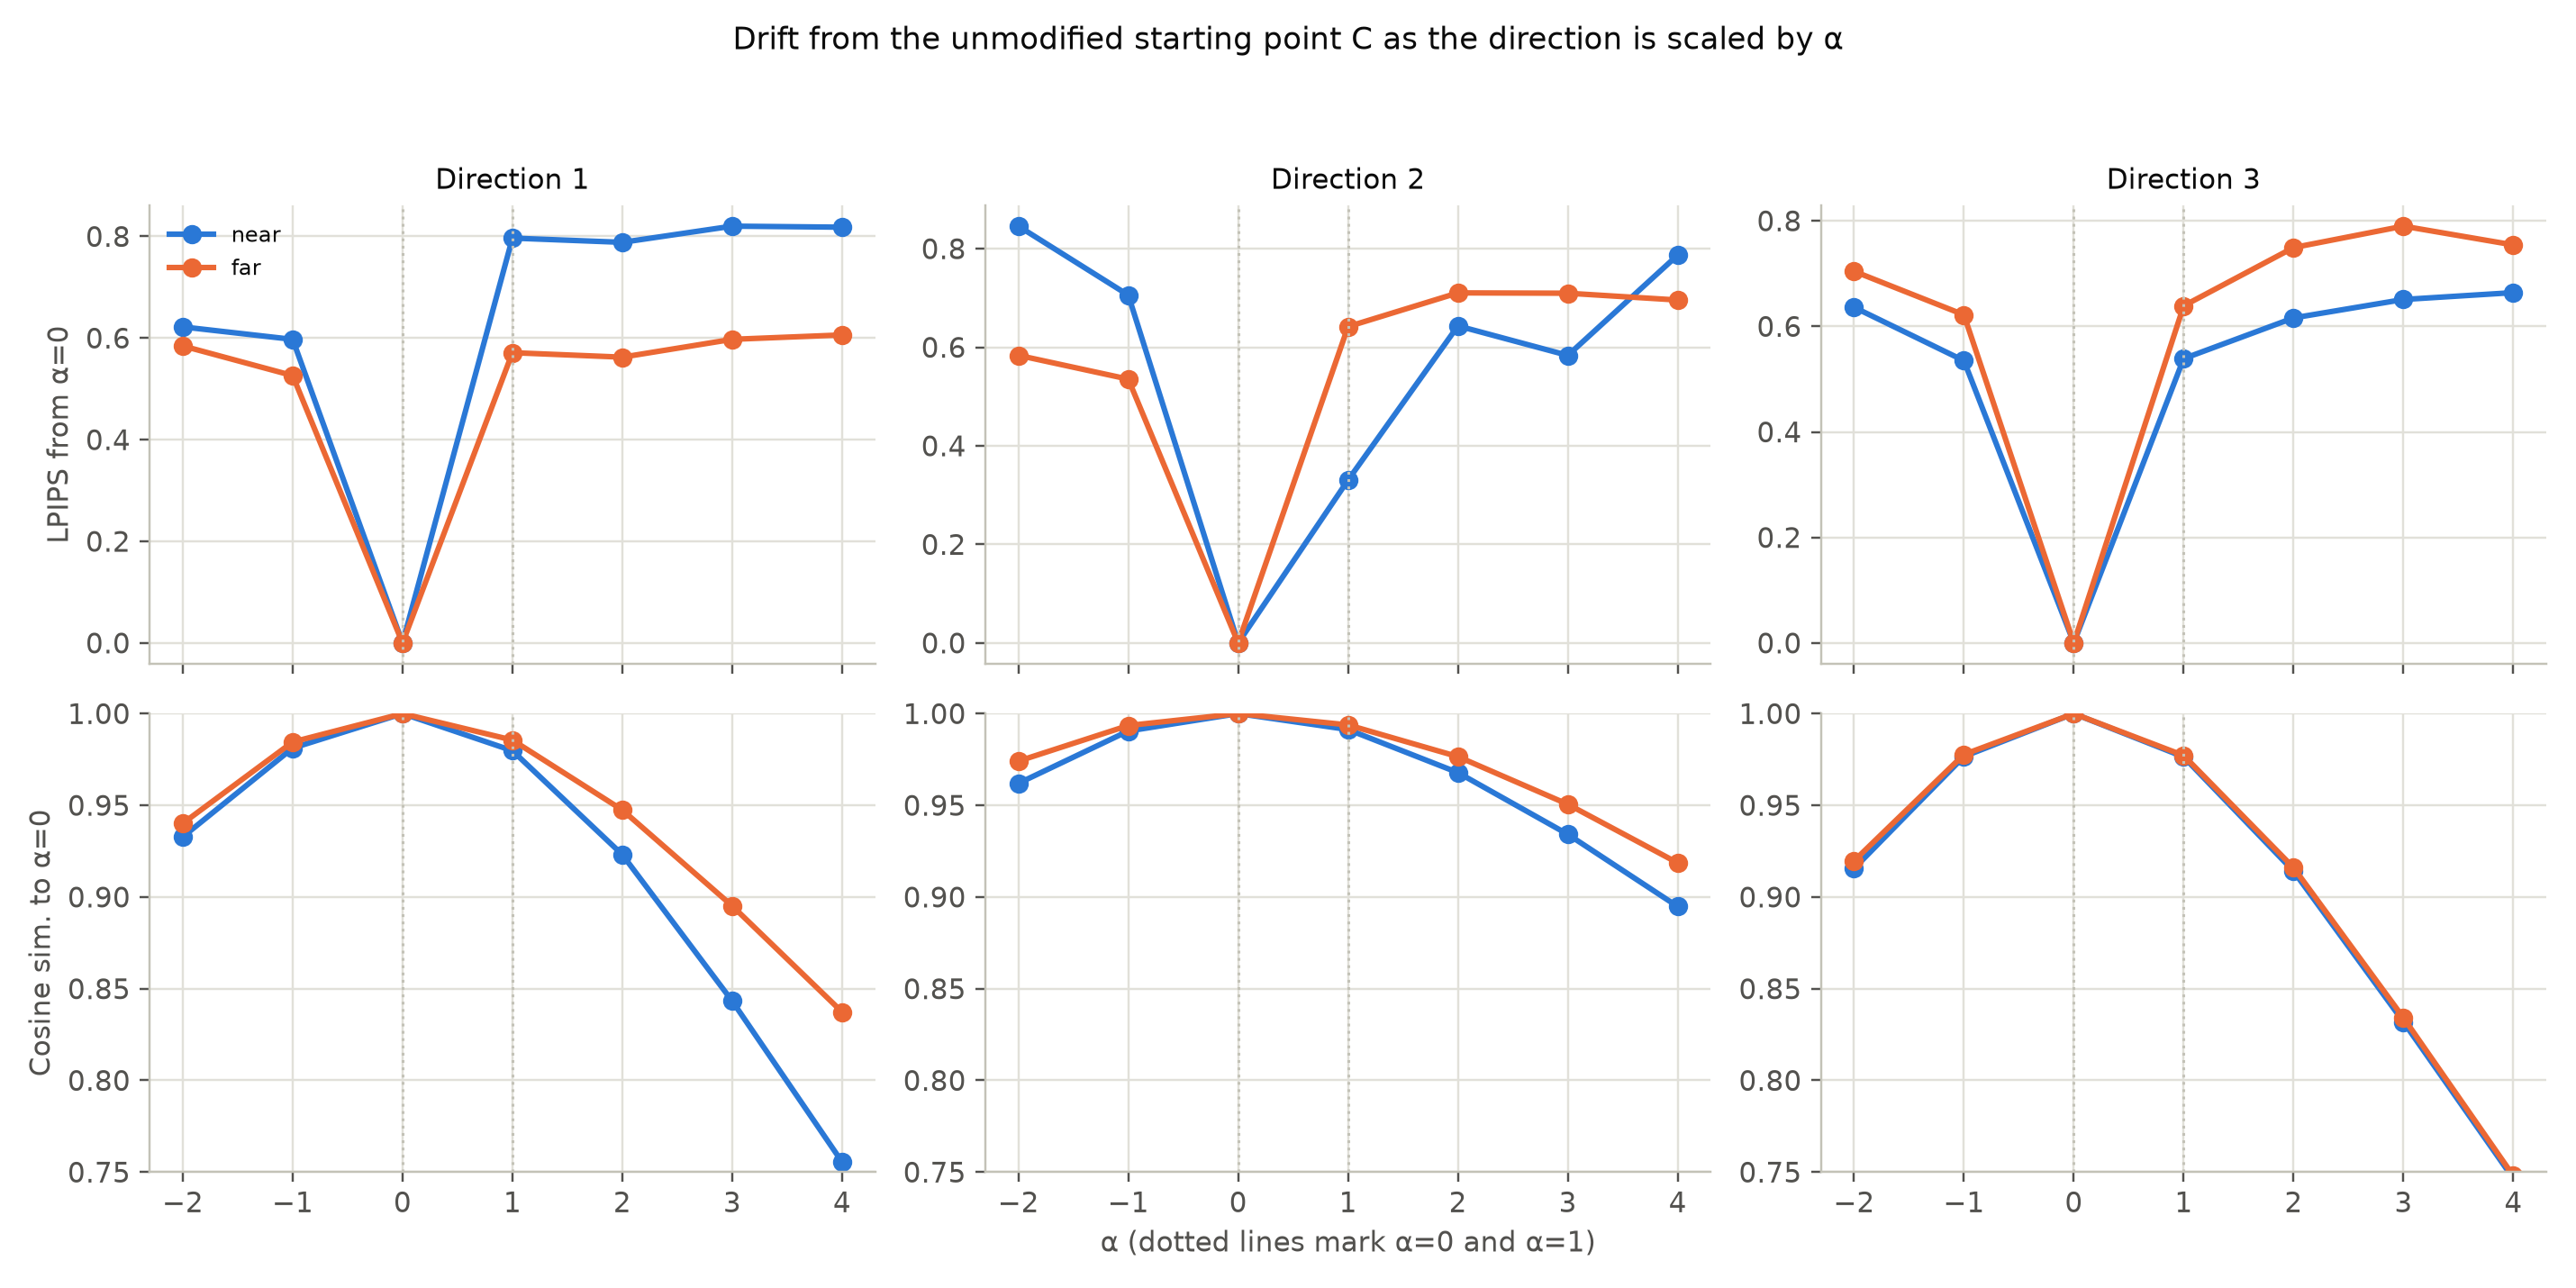
\includegraphics[width=0.9\textwidth]{figures/delta-walk-baseline-drift.png}
\caption{Baseline-relative LPIPS and cosine similarity to the $\alpha=0$ step, across the full alpha schedule, near and far context}
\label{fig:delta-walk-baseline-drift}
\end{figure}

How far a point moves in compact embedding space does not reliably predict how much the generated image changes perceptually, as shown in \hyperref[tbl:delta-walk-summary]{Table~\ref*{tbl:delta-walk-summary}}. For all six walks, the minimum baseline cosine similarity occurs at $\alpha=4$: since the tested schedule reaches further forward (to $\alpha=4$) than in reverse (to $\alpha=-2$), this is simply the largest-magnitude step tested, not a special property of that particular alpha. However, the maximum baseline LPIPS value, which identifies the greatest perceptual deviation from the starting image, occurs at the same step in only two cases. In the remaining four walks, perceptual change peaks earlier. The clearest example is the near context of Direction 2, where the highest LPIPS value occurs at $\alpha=-2$, although \hyperref[fig:delta-walk-baseline-drift]{Figure~\ref*{fig:delta-walk-baseline-drift}} shows the compact embedding remains relatively close to its baseline there, with a cosine similarity of approximately 0.96.

The baseline cosine-similarity curves in \hyperref[fig:delta-walk-baseline-drift]{Figure~\ref*{fig:delta-walk-baseline-drift}} are approximately symmetric around $\alpha=0$ for equal movement in opposite directions: moving away from C by the same amount in either direction changes the result's angle from its baseline by a similarly small or large amount, so applying the same direction vector with opposite signs produces near-identical cosine similarity to the baseline. Baseline LPIPS does not exhibit a comparable symmetry. Its values rise and fall unevenly across the schedule, reflecting the mismatch between the points of maximum embedding displacement and maximum perceptual change observed in the summary table.

Together, these measures distinguish the geometric behavior of the operation from its visual outputs. Movement in compact embedding space follows the expected directional pattern and is approximately symmetric for equal positive and negative values of $\alpha$. The generated images, however, do not respond proportionally or symmetrically to this movement. Their greatest perceptual deviation may occur before the largest embedding displacement or even at the opposite end of the tested range. This suggests that the diffusion model maps similar geometric displacements to visual changes in a nonlinear and context-dependent manner.

The largest local perceptual transition, measured as the maximum LPIPS value between consecutive steps and shown in \hyperref[fig:delta-walk-step-profile]{Figure~\ref*{fig:delta-walk-step-profile}}, also varies across the $\alpha$ schedule and does not consistently align between the near and far contexts of the same direction. For Direction 1, the near context exhibits its strongest transition between $\alpha=0$ and $\alpha=1$, whereas the far context reaches a smaller maximum at the opposite end of the schedule, between $\alpha=3$ and $\alpha=4$. For Direction 2, both contexts peak relatively early: the near context between $\alpha=-2$ and $\alpha=-1$, and the far context between $\alpha=0$ and $\alpha=1$. Direction 3 shows another pattern, with the near context peaking between $\alpha=-2$ and $\alpha=-1$ and the far context between $\alpha=1$ and $\alpha=2$.

Across the six walks, no single interval consistently represents the most abrupt transition. Even when the same direction is applied, its near and far contexts may reach their maximum perceptual change in widely separated parts of the schedule. This contrasts with the LERP and SLERP results in \hyperref[sec:5.3]{Section~5.3}, where the strongest transition occurred within the same interior interval for both methods applied to a given prompt pair. The variability observed here is consistent with the qualitative results discussed below: depending on the starting context, a transferred direction may produce a clear transformation, have only a limited visible effect, or introduce an unrelated subject.

\begin{figure}[htbp]
\centering
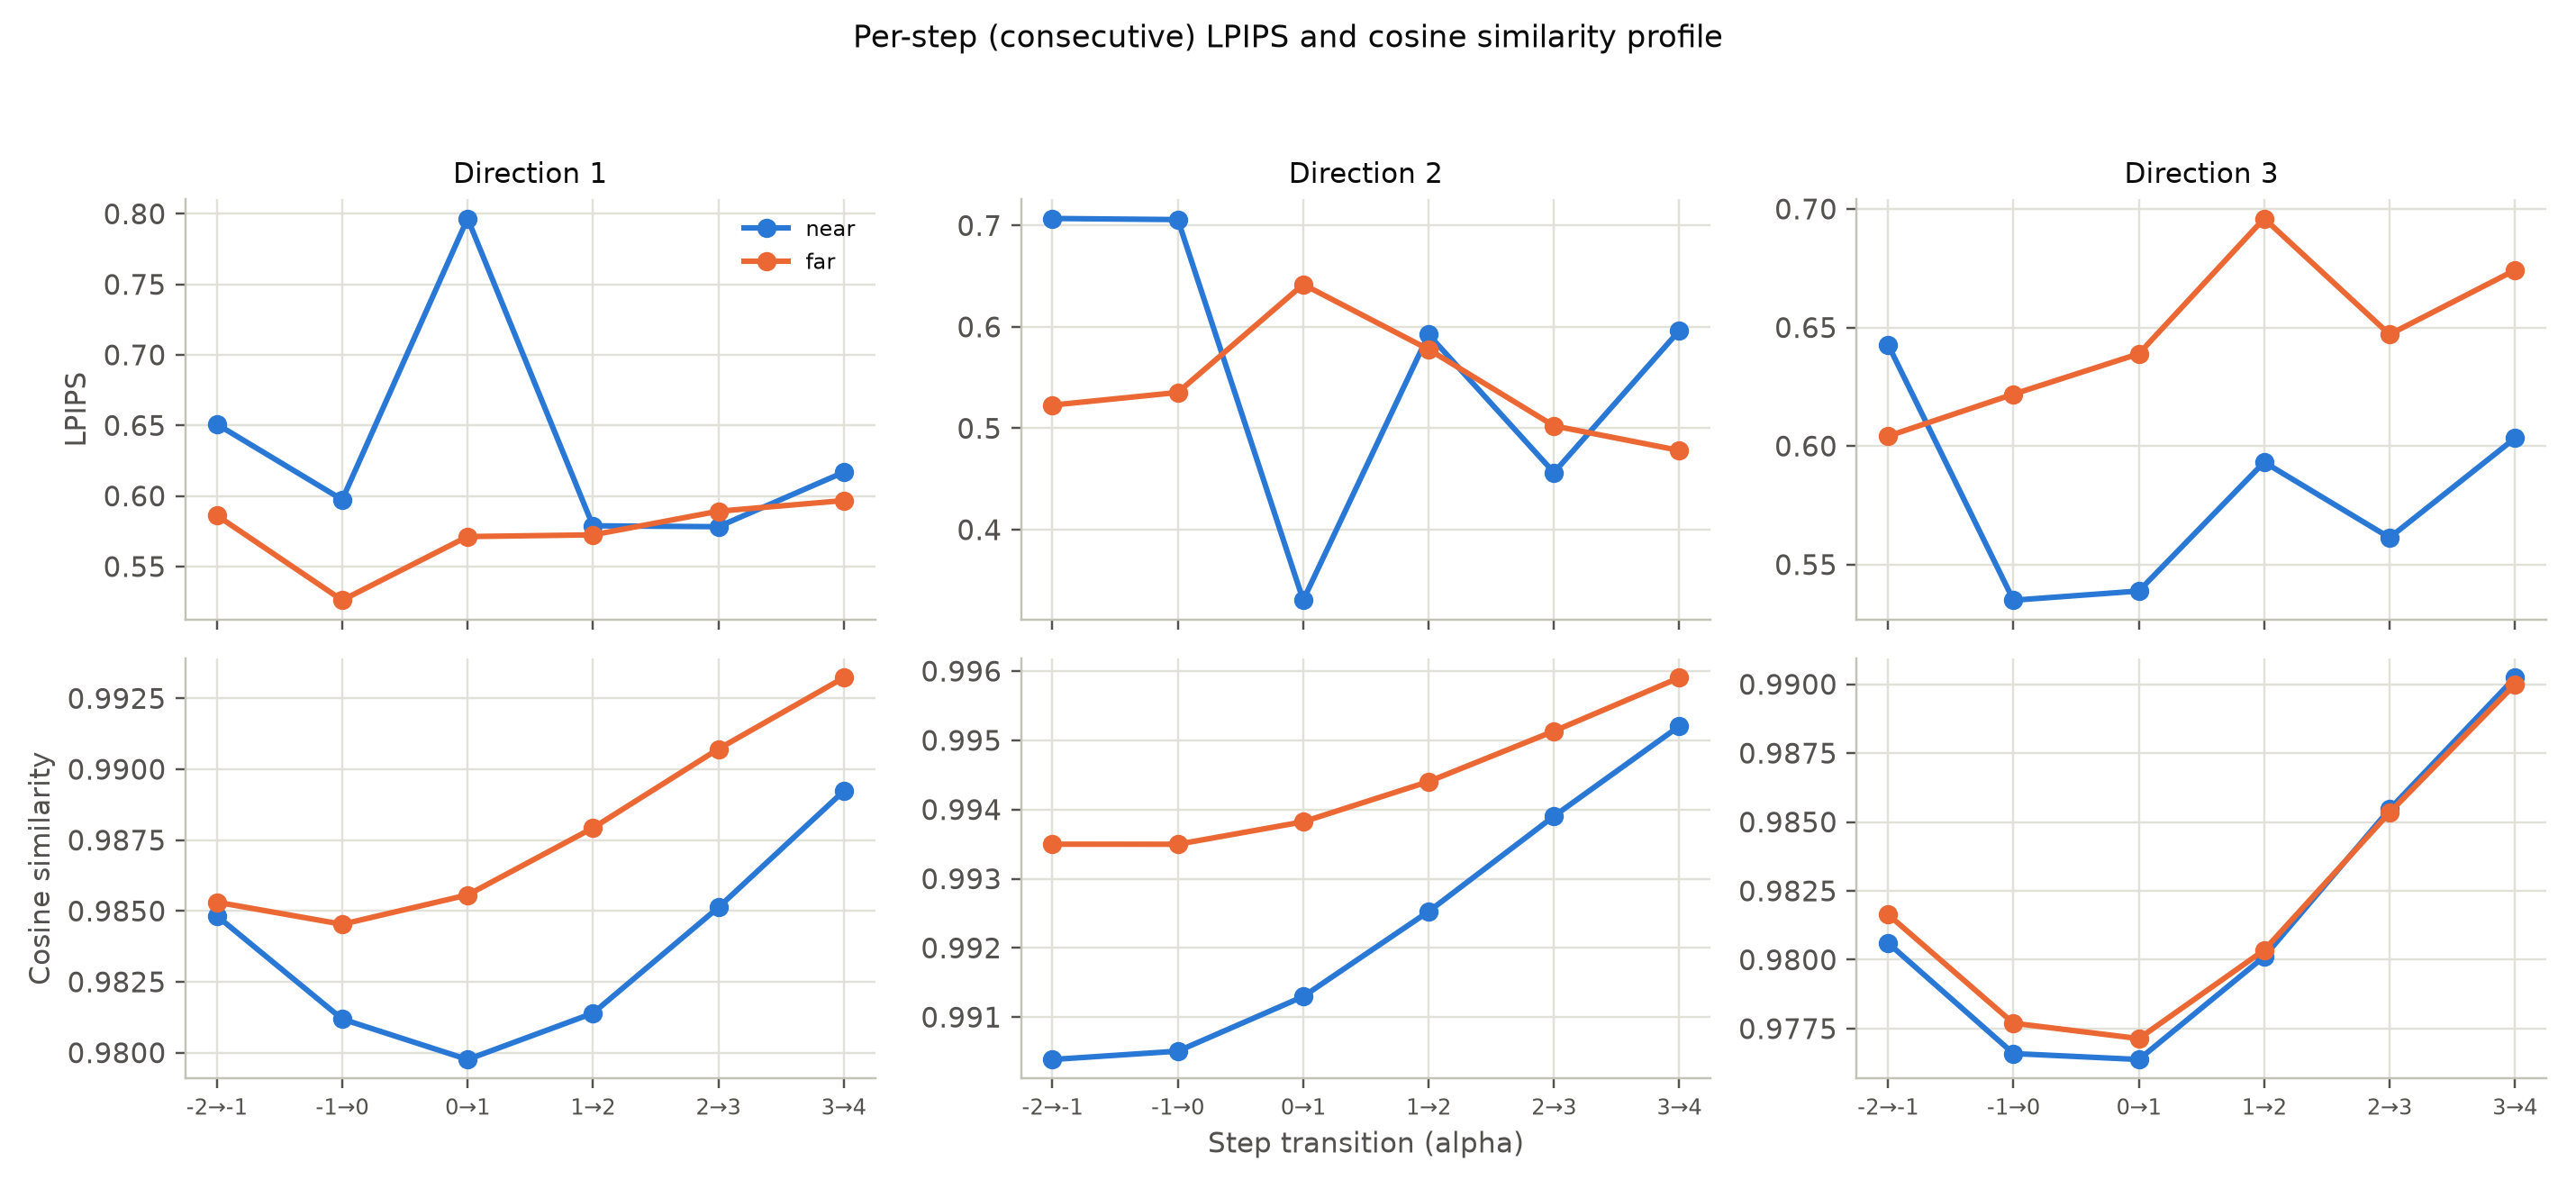
\includegraphics[width=0.9\textwidth]{figures/delta-walk-step-profile.png}
\caption{Per-step (consecutive) LPIPS and cosine similarity profile across the six step transitions, near and far context}
\label{fig:delta-walk-step-profile}
\end{figure}

A structured qualitative review of the endpoints and the highest-LPIPS transition in each of the six walks supports this interpretation. Direction 2, defined by the transformation from shoes to a jacket (\hyperref[fig:delta-walk-strip-direction2]{Figure~\ref*{fig:delta-walk-strip-direction2}}), produces the most consistently coherent behavior. In both contexts, the original product remains recognizable across the full range, while increasing $\alpha$ introduces progressively stronger weathering, patchwork, and armor-like detailing. The subject itself is not replaced, although some steps place the product on a humanoid model.

Direction 1, representing cyberpunk styling (\hyperref[fig:delta-walk-strip-direction1]{Figure~\ref*{fig:delta-walk-strip-direction1}}), transfers successfully to the near context. As $\alpha$ increases, the fox acquires increasingly pronounced cybernetic components and neon-lit details while remaining identifiable. In the far context, however, the seaside village is replaced by an unrelated humanoid figure at $\alpha=3$ and $\alpha=4$, rather than being transformed into a cyberpunk interpretation of the same scene. A possible explanation is that the village provides no clear visual subject to which cybernetic components can be attached, leading the model to introduce a person who can carry the transferred attribute.

Direction 3, representing an identity transformation (\hyperref[fig:delta-walk-strip-direction3]{Figure~\ref*{fig:delta-walk-strip-direction3}}), also transfers clearly to its near context, which contains another named person. Skin tone and styling change in the expected direction, while the original sorceress or warrior composition remains recognizable throughout the walk. The far context, an umbrella, cannot express the identity-related component of the direction, and no real person appears at any value of $\alpha$. Nevertheless, the object becomes progressively more ornate, jeweled, and gold-toned as $\alpha$ increases. These changes reflect stylistic qualities shared by the two anchor prompts, such as ornamentation and intricacy, even though the identity attribute itself has no compatible subject on which to act. In this case, the conditioning of the starting prompt preserves the original object while allowing only semantically compatible aspects of the transferred direction to appear.

\begin{figure}[htbp]
\centering
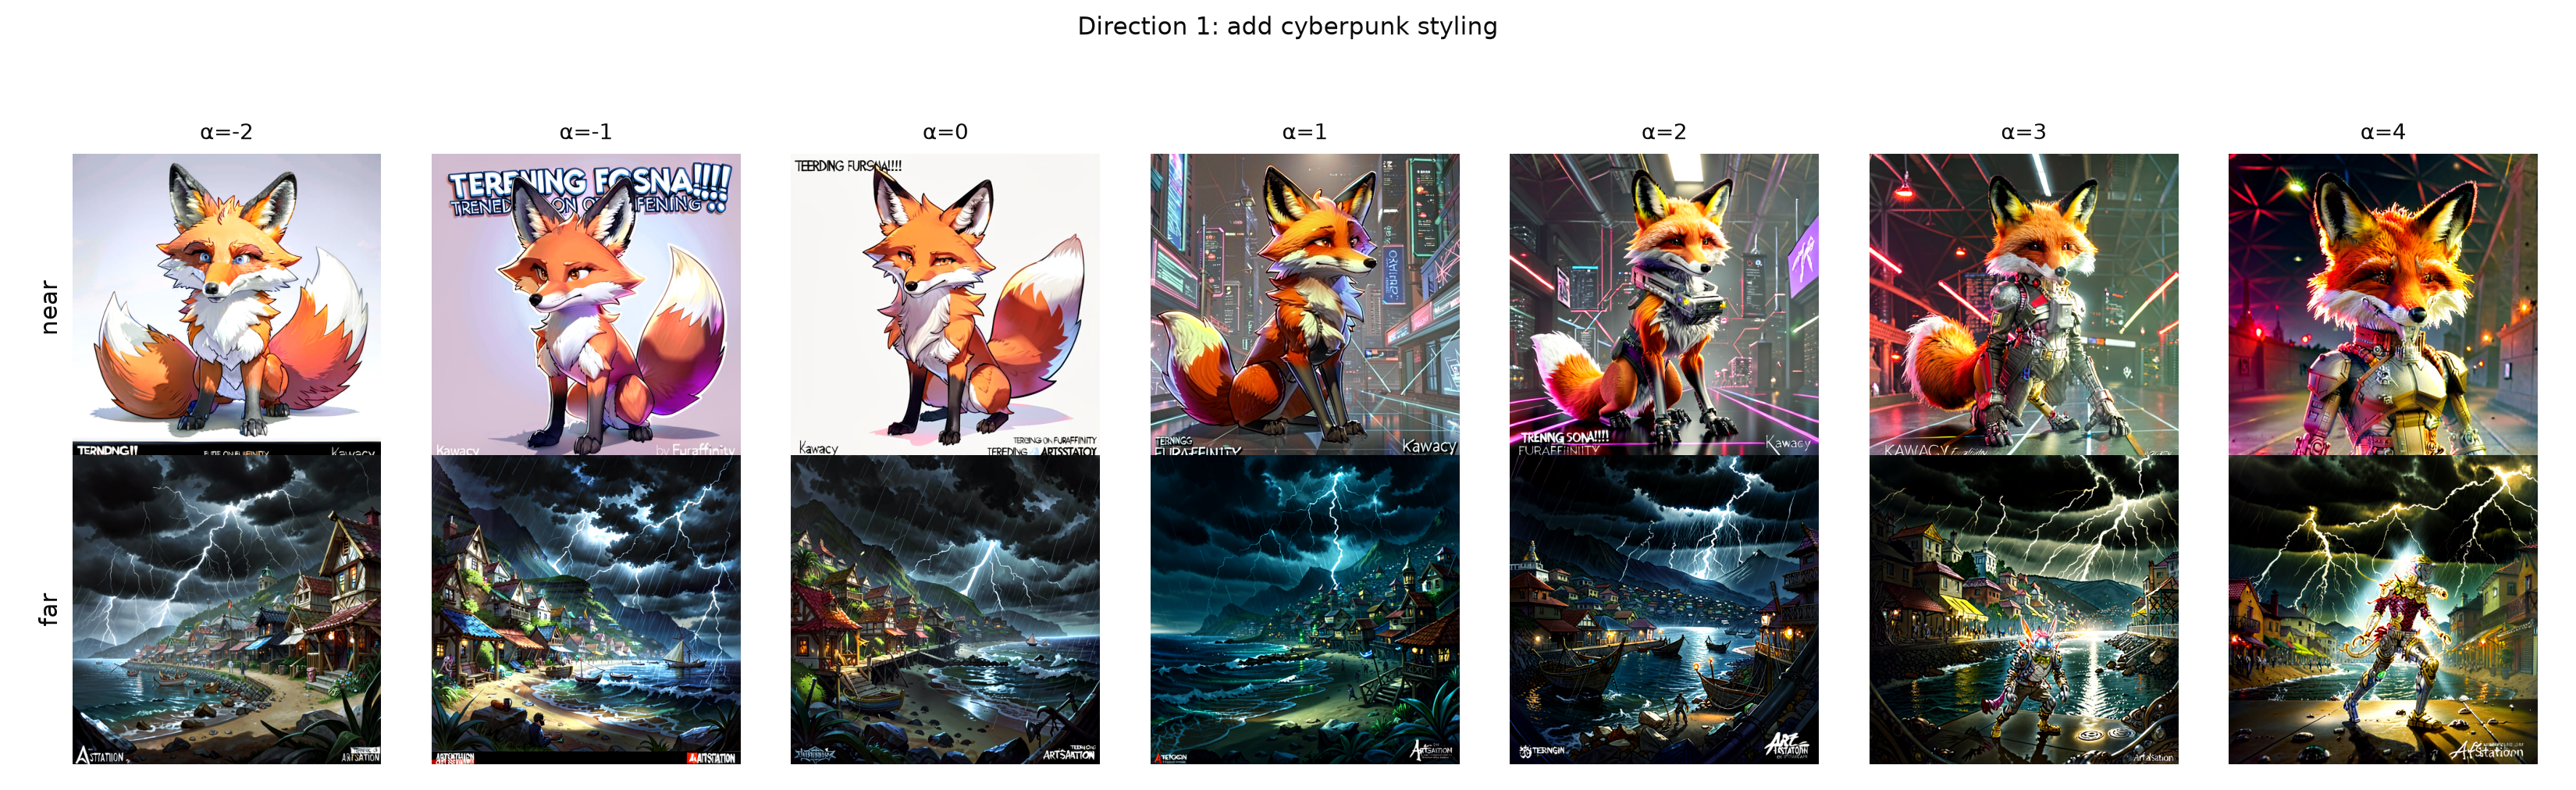
\includegraphics[width=\textwidth]{figures/delta-walk-strip-direction1.png}
{\setstretch{1.0}
\caption[Direction 1 (add cyberpunk styling), near and far context across the full alpha schedule]{Direction 1 (add cyberpunk styling), near and far context across the full alpha schedule. A: "a fox fursona, trending on artstation, by kawacy, furry art, digital art". B: "a fox fursona, trending on artstation, by kawacy, furry art, digital art, cyberpunk, high quality, backlighting". Near C: "an anthropomorphic fox, fursona!!!! trending on furaffinity, by kawacy, trending on artstation". Far C: "a seaside village, detailed, fantasy style, stormy day, trending on artstation"}
\label{fig:delta-walk-strip-direction1}
}
\end{figure}

\begin{figure}[htbp]
\centering
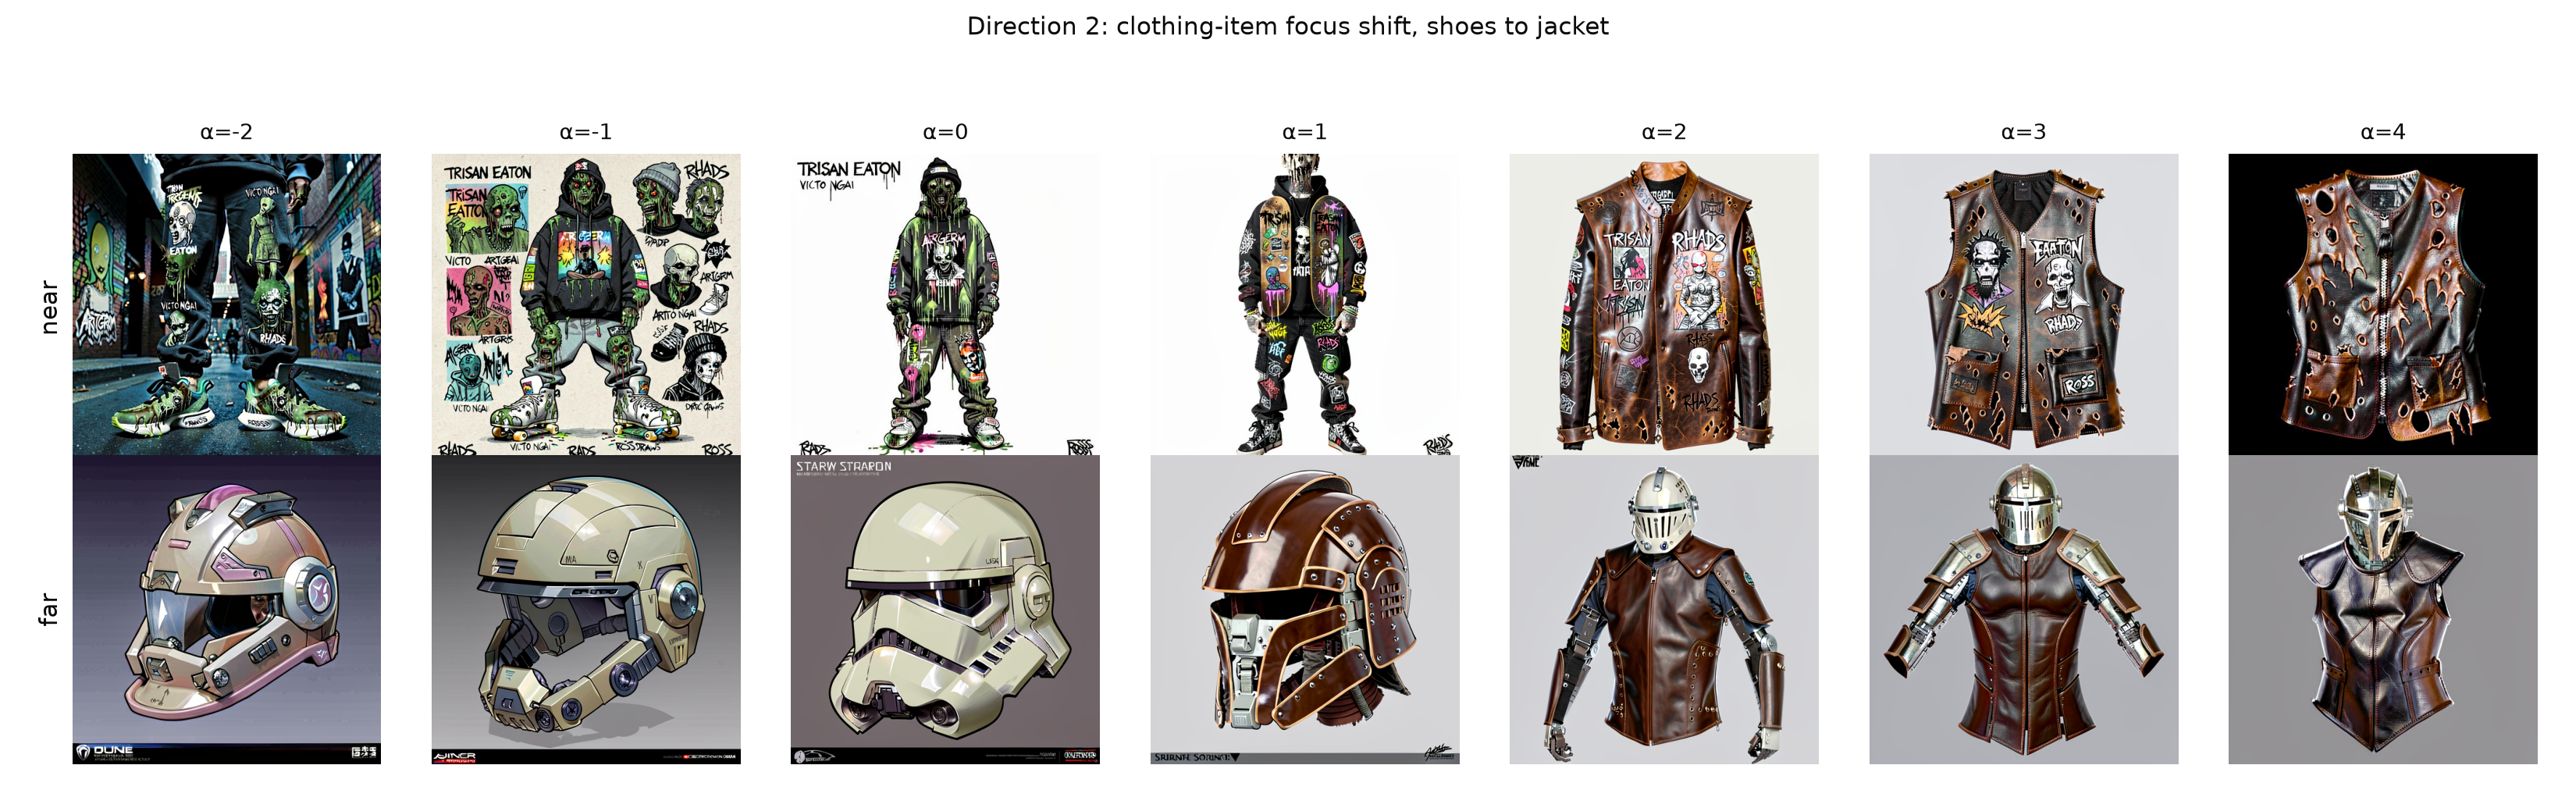
\includegraphics[width=\textwidth]{figures/delta-walk-strip-direction2.png}
{\setstretch{1.0}
\caption[Direction 2 (shoes to jacket focus shift), near and far context across the full alpha schedule]{Direction 2 (shoes to jacket focus shift), near and far context across the full alpha schedule. A: "zombie jordan shoes female hiphop streetwear drip, tristan eaton, victo ngai, artgerm, rhads, ross draws". B: "zombie leather jacket full body hiphop streetwear drip, tristan eaton, victo ngai, artgerm, rhads, ross draws". Near C: "zombie skateboard full body hiphop streetwear drip, tristan eaton, victo ngai, artgerm, rhads, ross draws". Far C: "new stormtrooper/clone trooper helmet design, concept art"}
\label{fig:delta-walk-strip-direction2}
}
\end{figure}

\begin{figure}[htbp]
\centering
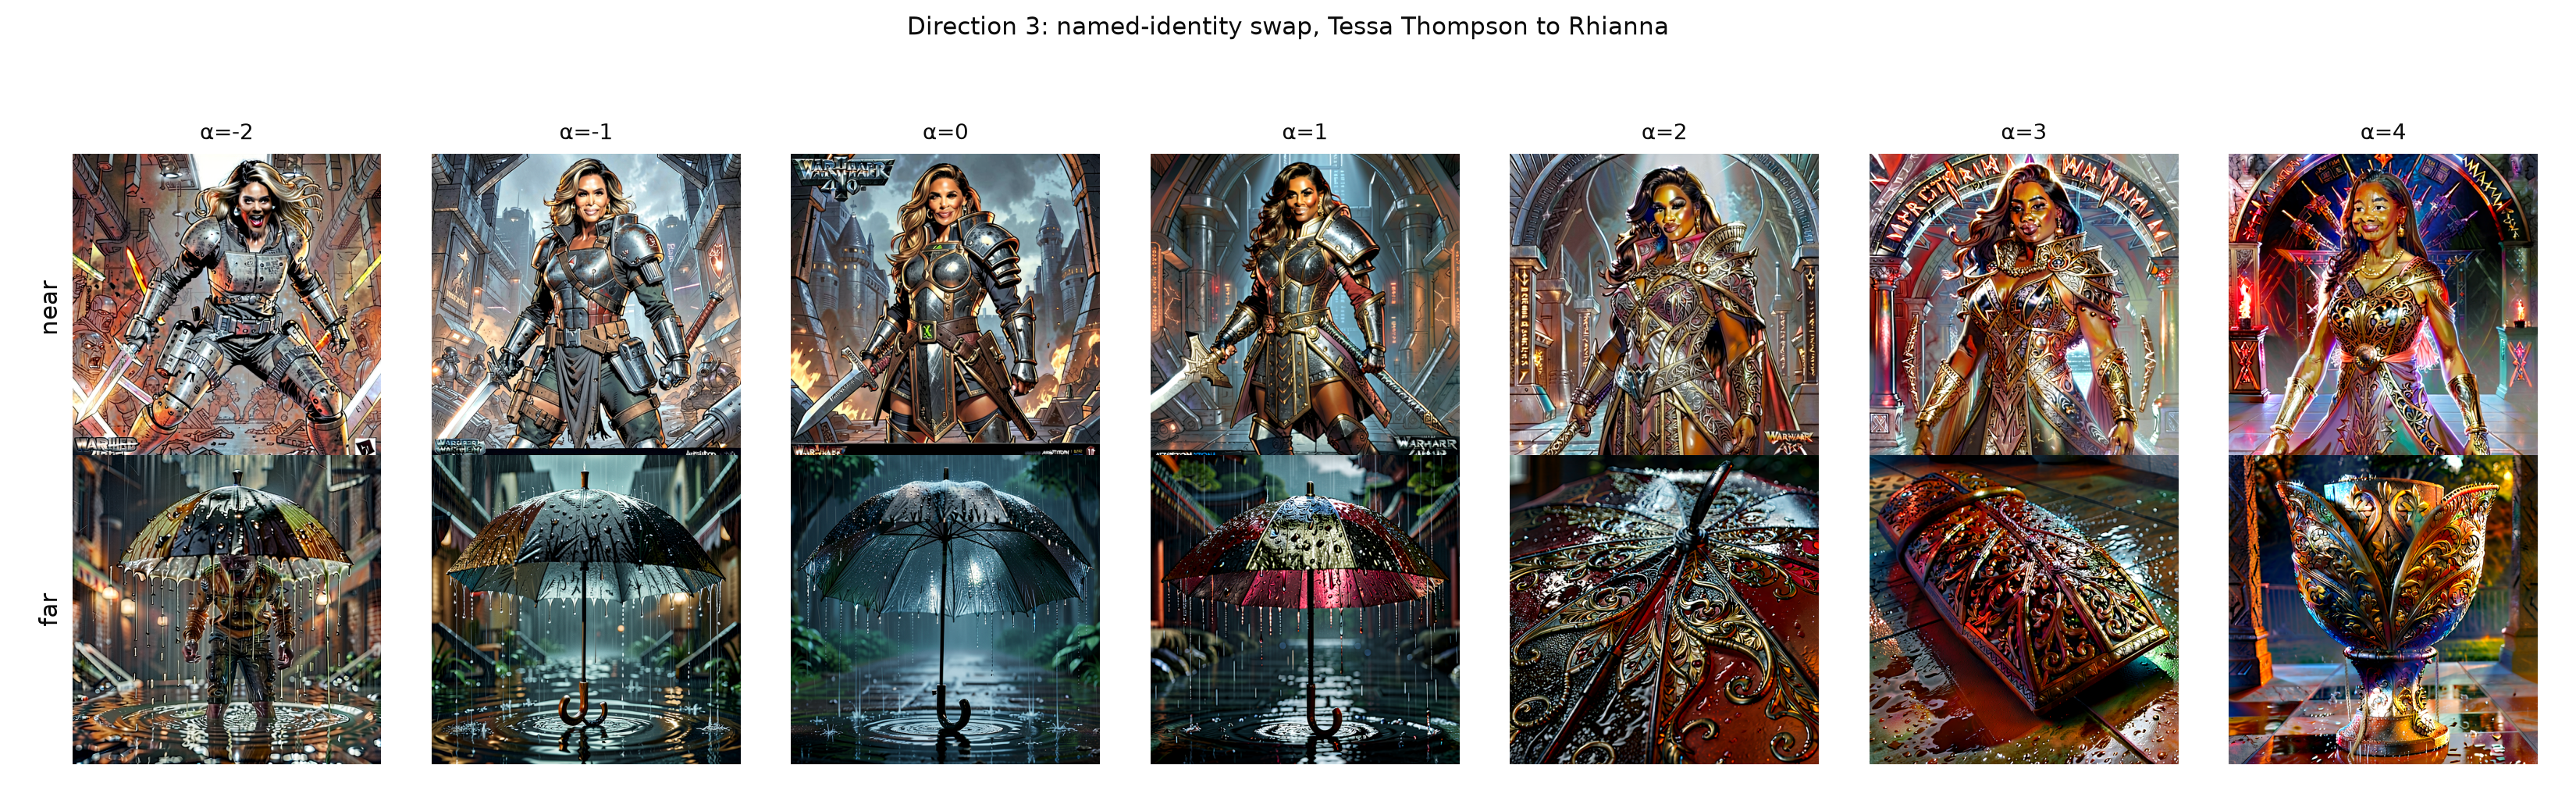
\includegraphics[width=\textwidth]{figures/delta-walk-strip-direction3.png}
{\setstretch{1.0}
\caption[Direction 3 (named-identity swap), near and far context across the full alpha schedule]{Direction 3 (named-identity swap), near and far context across the full alpha schedule. A: "Tessa Thompson as a sorceress, passionate, seductive, sweaty, intricate dressed in ornate blue robes and staff, insane, intricate,". B: "Rhianna as a sorceress, passionate, seductive, sweaty, intricate dressed in ornate blue robes and staff, intricate,". Near C: "Sofia Vergara as a battle sister from Warhammer 40k, highly detailed, intricate, concept art, artstation". Far C: "An umbrella, extreme detailed, wet, photorealistic, octane render, 8k, by greg rutkowski and studio ghibli"}
\label{fig:delta-walk-strip-direction3}
}
\end{figure}

Finally, each direction's A/B anchors and both walks were projected into \texttt{gustavosta\_sd\_prompts\_v2\_two\_pass}'s own runtime reducer, the same one used in the previous section. The 2D figure plots this against all 61.746 of the dataset's own canonical positions for context and, new for this section, the A-to-B direction itself drawn as a reference arrow. The 3D figure instead zooms into each walk's own neighborhood.

\begin{figure}[htbp]
\centering
\begin{subfigure}[b]{\textwidth}
\centering
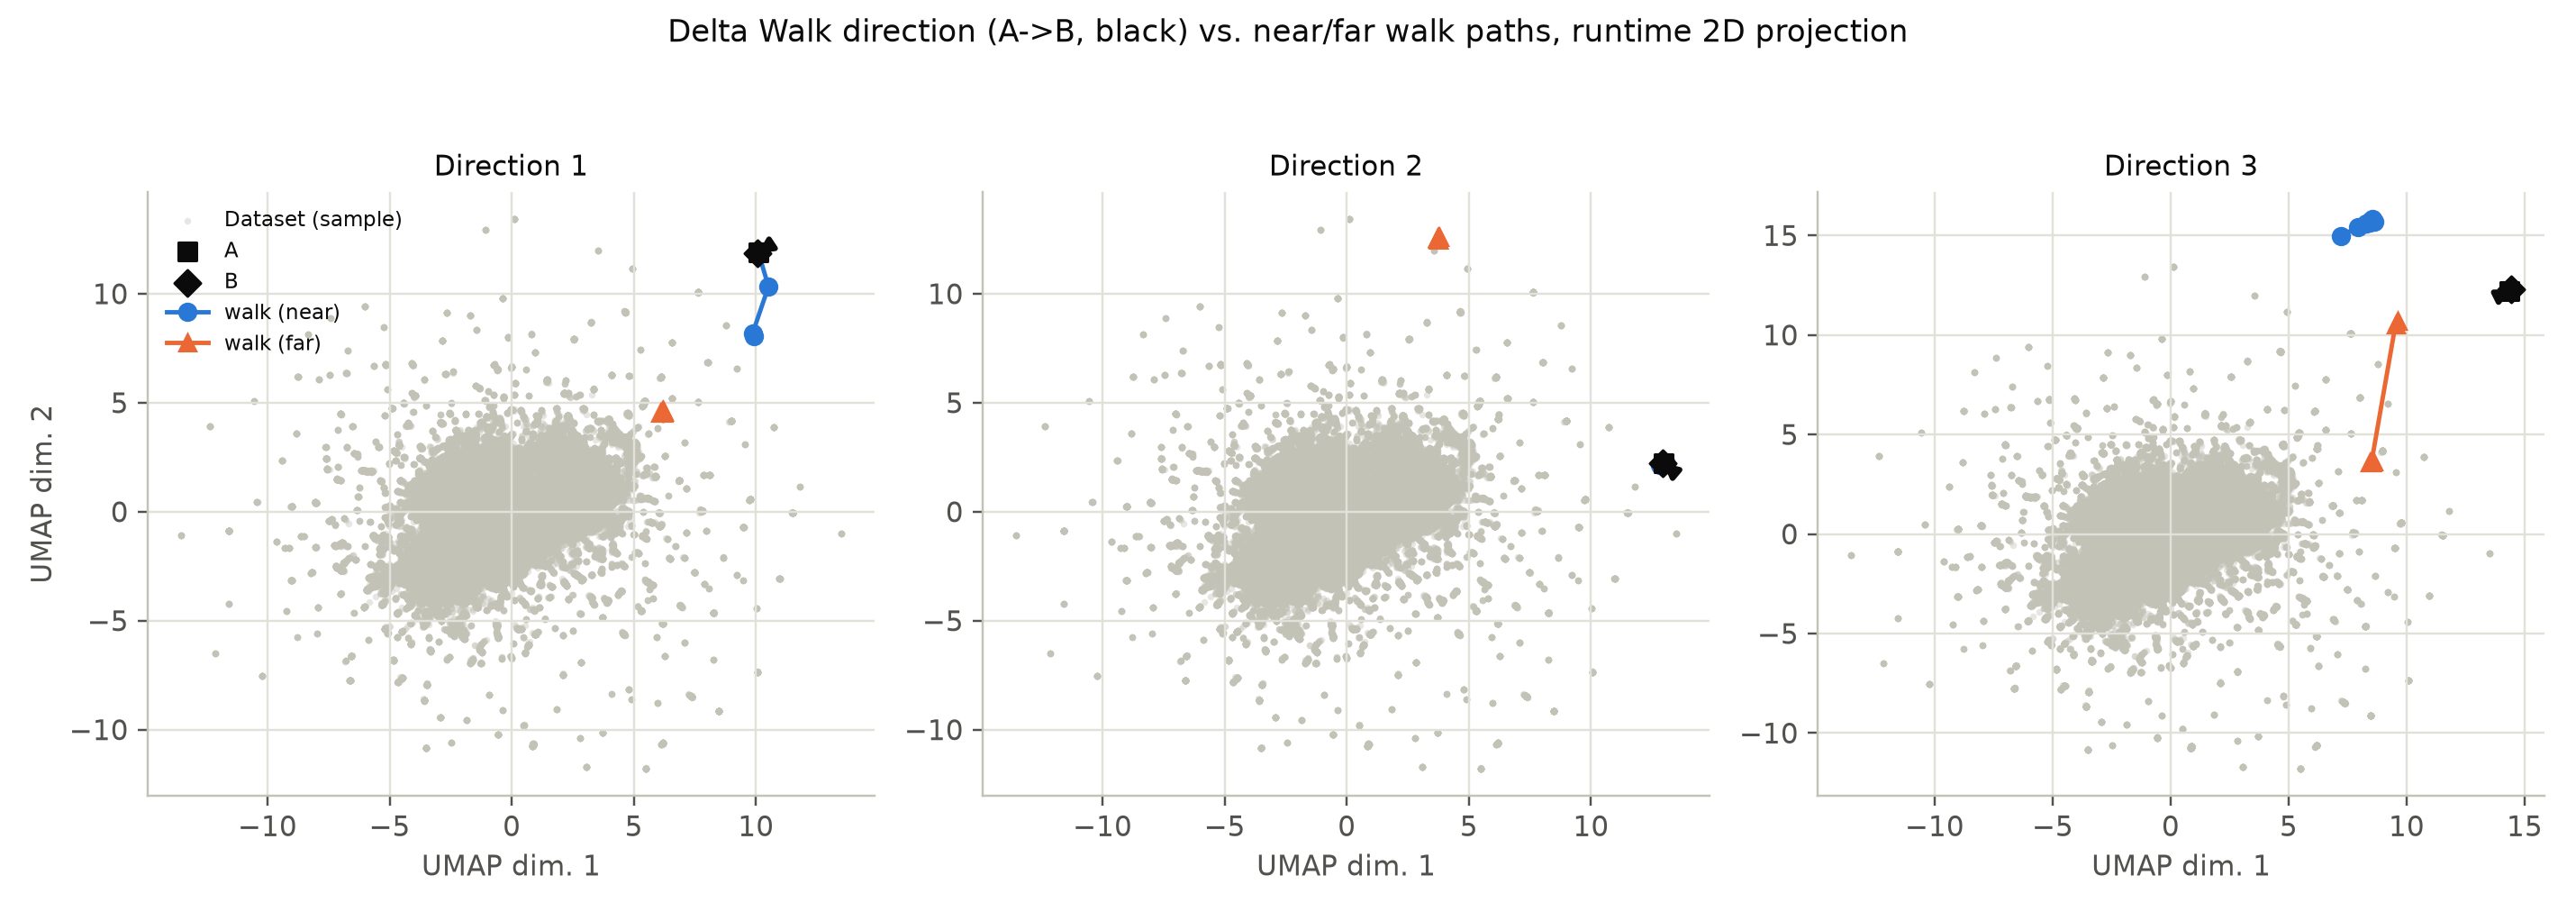
\includegraphics[width=0.9\textwidth]{figures/delta-walk-trajectory-graph-2d.png}
\caption{The A$\to$B direction (black arrow) and both walks' projected positions}
\label{fig:delta-walk-trajectory-graph-2d}
\end{subfigure}
\begin{subfigure}[b]{\textwidth}
\centering
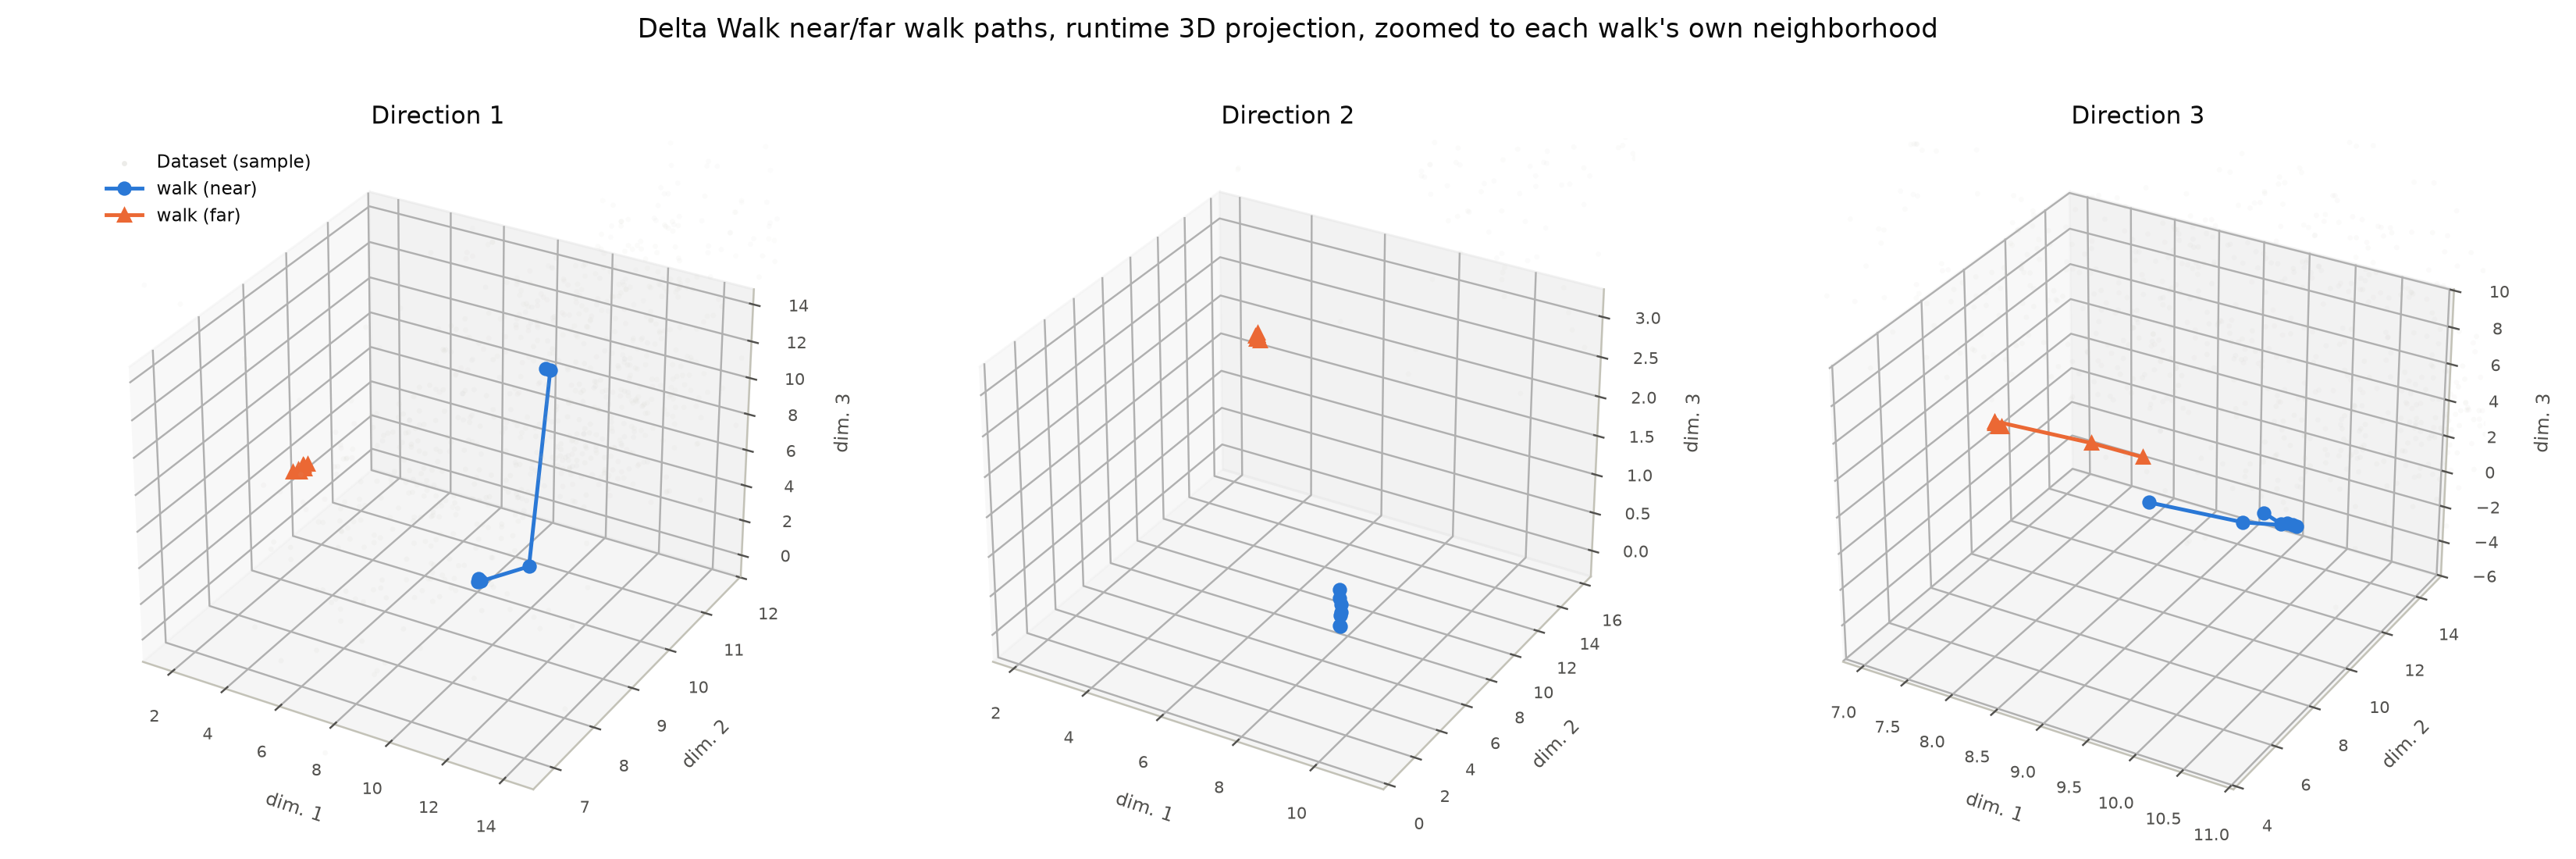
\includegraphics[width=0.9\textwidth]{figures/delta-walk-trajectory-graph-3d.png}
\caption{The same three directions, axis limits zoomed to each walk's own neighborhood}
\label{fig:delta-walk-trajectory-graph-3d}
\end{subfigure}
\caption{Delta/Direction Walk anchors and both walks' projected positions, runtime 2D and 3D reducer output}
\label{fig:delta-walk-trajectory-graph}
\end{figure}

In the two-dimensional projection, both anchor prompts and the trajectories generated from them lie outside the main density region of the dataset, reproducing the pattern observed for the interpolation trajectories in \hyperref[sec:5.3]{Section~5.3}. Even at $\alpha=4$, the seven projected points of each walk cover only a short distance relative to both the corresponding A-to-B direction and the surrounding point cloud. The three-dimensional view in \hyperref[fig:delta-walk-trajectory-graph-3d]{Figure~\ref*{fig:delta-walk-trajectory-graph-3d}} makes this limited displacement more visible. Each trajectory remains close to its position at $\alpha=0$, even in cases where \hyperref[fig:delta-walk-baseline-drift]{Figure~\ref*{fig:delta-walk-baseline-drift}} shows substantial perceptual change in the generated images. Large image-level changes therefore do not necessarily require a similarly large displacement in the projected compact embedding space.

\hyperref[fig:delta-walk-trajectory-graph-2d]{Figure~\ref*{fig:delta-walk-trajectory-graph-2d}} and \hyperref[fig:delta-walk-trajectory-graph-3d]{Figure~\ref*{fig:delta-walk-trajectory-graph-3d}} further show that the near and far contexts of the same direction occupy distinct neighborhoods rather than different positions within a shared local region. For all three directions, the projected points of each walk remain more closely grouped with their own starting context than with the other context to which the same direction was applied. This pattern also holds for the near context of Direction 1, which exhibits the greatest internal spread among the six walks: its points still form a recognizable local group that remains separate from the corresponding far-context trajectory. Neither the projected path length of an individual walk nor the separation between the near- and far-context trajectories provides a direct measure of semantic transfer quality. This reinforces the mismatch between projected geometry and perceptual content observed earlier in this section and in \hyperref[sec:5.3]{Section~5.3}. Whether a transferred direction remains semantically meaningful must therefore be assessed from the generated images rather than inferred from the projection alone.

Within this experimental setup, Direction Walk produces approximately smooth and symmetric movement in compact embedding space across the tested $\alpha$ range. The corresponding perceptual changes, however, are neither symmetric nor consistently strongest at the most extreme extrapolation values. The results further show that the semantic structure of the starting context can weaken, redirect, or absorb a transferred direction instead of expressing it as a direct attribute change.

For users applying Direction Walk as a semantic-editing method, neither the extrapolation strength nor the geometric symmetry of the operation provides a reliable indication of how strongly or predictably the edit will appear in the generated image. The outcome depends largely on whether the starting context is compatible with the transferred attribute. Contexts that share conceptual similarities with the original anchor pair are more likely to express the direction as a coherent and controllable edit, whereas unrelated contexts may weaken the effect, distort the result, or replace the original subject entirely.

\FloatBarrier
\section{Semantic Axis Projection}\label{sec:5.5}

\hyperref[sec:4.8]{Section~4.8} introduced Semantic Axis Projection, in which users select two groups of points representing opposite poles of a semantic contrast. All loaded points are then assigned a score along the primary axis connecting these groups. The operation may additionally derive a second axis from the residual variation not explained by the first. As emphasized in \hyperref[sec:4.8]{Section~4.8}, these axes are exploratory and depend on the selected examples and dataset. They should therefore be understood as approximations of semantic structure rather than universal semantic measures. Building on this limitation, the present section addresses two narrower questions: whether a primary axis based on only a few example points still applies to unseen points sharing the same theme, and whether the automatically derived second axis has a meaningful interpretation.

Two semantic contrasts were constructed using the canonical clustering of \texttt{gustavosta\_sd\_prompts\_v2\_two\_pass} as an independent, dataset-specific reference for thematic membership. The target clusters were selected by inspecting representative prompts from the largest clusters. The first contrast is a semantically near pair consisting of cyberpunk prompts from cluster 70, containing 531 members, and steampunk prompts from cluster 23, containing 338 members. These clusters represent visually related "-punk" aesthetics. The second is a semantically far pair consisting of dragon and monster prompts from cluster 99, containing 356 members, and fairytale architecture and interior prompts from cluster 109, containing 633 members. These clusters represent largely unrelated subject categories.

The generalization of the primary axis is evaluated using two complementary measures. For each target cluster, 20 members are selected randomly as anchors, while all remaining members are withheld from axis construction. The first measure evaluates whether the primary axis continues to separate these unseen samples, tested using the Mann-Whitney U test implemented by \texttt{scipy.stats.mannwhitneyu}. The null hypothesis states that a randomly selected held-out Group B member is no more likely to receive a higher score than a randomly selected held-out Group A member, meaning that thematic membership provides no information about a point's position on the axis. The alternative states that held-out members of Group B receive systematically higher scores than those of Group A, meaning that the axis correctly separates the two groups' held-out members by their true thematic membership, not only by the anchor points used to build it. The test compares every possible pair of one held-out Group A point and one held-out Group B point, and measures how often the Group B point scores higher. This proportion is equivalent to the area under the ROC curve (AUC): a value of 1 means perfect separation, while a value near 0.5 means the ranking is no better than chance. Unlike a fixed-threshold classification measure, this comparison remains informative when the score distributions are skewed or contain outliers. \cite{geeksforgeeks2024mannwhitney}

This result is not intended to show that the original HDBSCAN clusters are surprising or independently validated. Their assignments already derive from the geometry of the compact representations through the clustering pipeline described in \hyperref[sec:4.6]{Section~4.6}. Instead, the test asks whether a single direction estimated from only 20 examples per side preserves enough of that higher-dimensional thematic structure to order previously unseen cluster members correctly.

Support-band precision provides a second test of primary-axis generalization. Rather than considering the complete score distribution, it evaluates the extreme regions that the operation exposes for downstream analysis, including contrastive axis-term extraction. Even an axis that separates the target groups correctly would have limited practical value if its extreme bands were dominated by unrelated samples.

For this evaluation, the 20 anchors from each target cluster are supplied to the axis-construction procedure together with all held-out members of both clusters and a background sample of 4.000 points drawn randomly from neither target cluster. Anchors, held-out members, and background samples are therefore scored and ranked jointly, resulting in approximately 4.900 to 5.000 loaded points for each semantic contrast. At this scale, the support-band rule introduced in \hyperref[sec:4.8]{Section~4.8}, 10 percent of the loaded points, constrained to a minimum of 24 and a maximum of 80, selects the maximum of 80 points at each pole.

Including unrelated background samples gives non-target points a realistic opportunity to enter the extreme regions of the axis. Support-band precision is therefore defined as the proportion of the 80 points at a given pole that belong to the cluster represented by that pole. Points from the opposing target cluster and from the unrelated background sample count as incorrect assignments. Consequently, values below 1 represent contamination of the axis extremes.

The interpretability of the automatically derived second axis cannot be assessed through the same held-out procedure. Unlike the primary axis, the second axis is not defined by independently specified semantic groups. Its apparent poles are discovered from the residual variation itself, meaning that evaluating the axis against those same extremes would be circular. Its interpretation is therefore examined qualitatively after the corresponding axis results are presented later in this section.

\begin{table}[htbp]
\centering
\caption[Held-out separation and support-band precision per axis pair]{Held-out separation and support-band precision per axis pair. Anchor count is 20 per cluster throughout; held-out counts are the remainder of each cluster. Precision is followed by the number of background/unrelated points among the 80 band members}
\label{tbl:axis-projection-summary}
\resizebox{\textwidth}{!}{%
\begin{tabular}{|l|c|c|c|c|c|c|}
\hline
\textbf{Pair} & \textbf{Side A (n heldout)} & \textbf{Side B (n heldout)} & \textbf{Held-out AUC} & \textbf{Band-A prec. (bg./80)} & \textbf{Band-B prec. (bg./80)} & \textbf{Axis-2 var.} \\
\hline
1: cyberpunk vs. steampunk & steampunk (318) & cyberpunk (511) & 0.999 & 0.863 (11/80) & 1.000 (0/80) & 0.132 \\
\hline
2: creatures vs. fairytale architecture & creatures (336) & architecture (613) & 1.000 & 0.900 (8/80) & 0.975 (2/80) & 0.120 \\
\hline
\end{tabular}%
}
\end{table}

\begin{figure}[htbp]
\centering
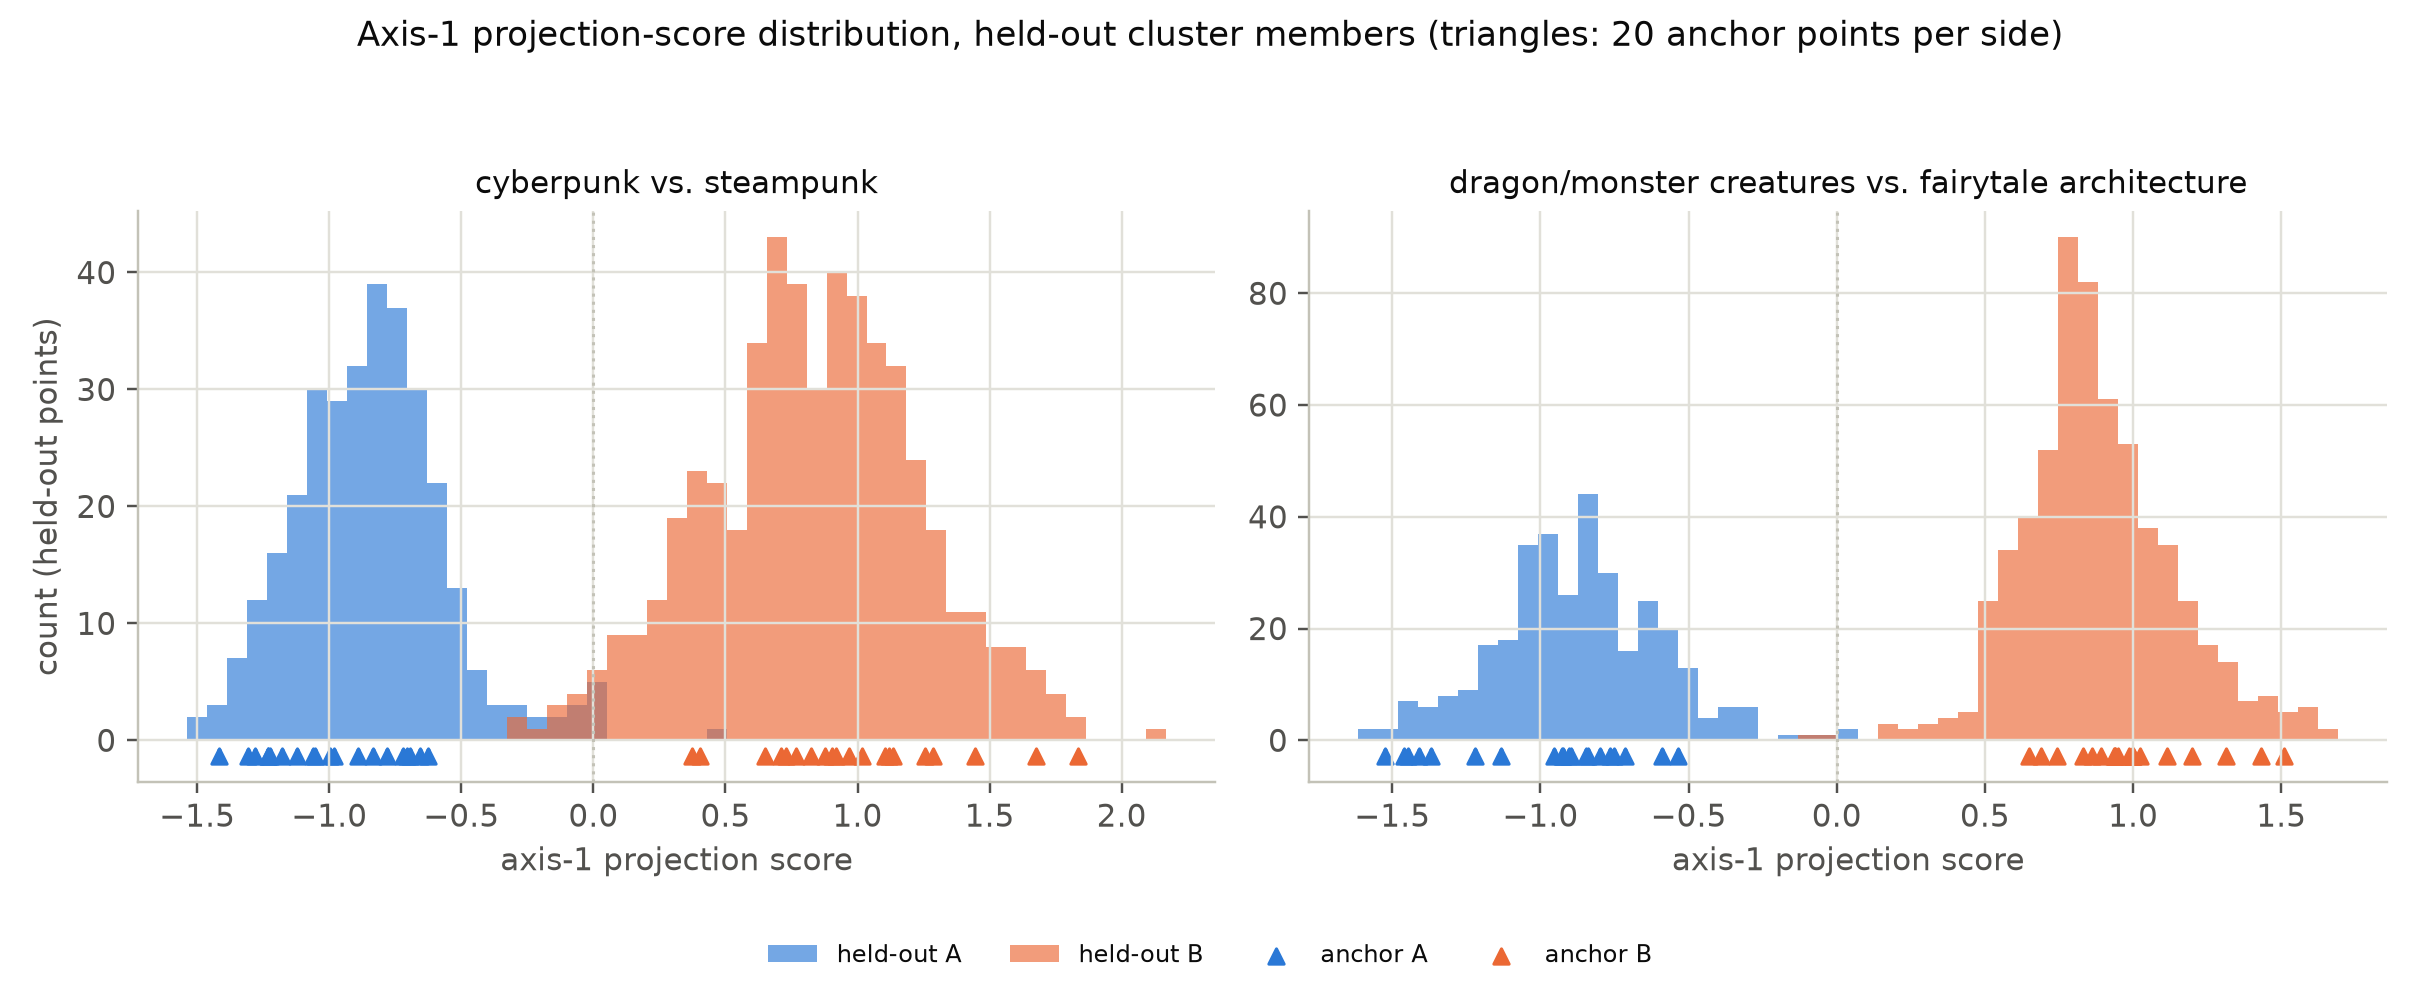
\includegraphics[width=0.9\textwidth]{figures/axis-projection-score-distribution.png}
\caption{Axis-1 projection-score distribution for held-out cluster members; triangles mark the 20 anchor points per side}
\label{fig:axis-projection-score-distribution}
\end{figure}

The near-perfect AUC values indicate that the primary axis generalizes strongly from only 20 anchor examples per side. As shown in \hyperref[fig:axis-projection-score-distribution]{Figure~\ref*{fig:axis-projection-score-distribution}}, the held-out samples from Groups A and B form almost completely separate score distributions. For pair 1, only a narrow overlap near the center of the axis prevents the AUC from reaching 1.000, resulting instead in 0.999. For pair 2, no visible overlap remains.

This statistical separation is supported by the axis terms extracted independently from the support bands. For pair 1, terms such as \texttt{steampunk}, \texttt{artstation}, and \texttt{trending} contrast with \texttt{cyberpunk}, \texttt{art}, and \texttt{concept}. For pair 2, \texttt{dragon}, \texttt{artstation concept}, and \texttt{art smooth} contrast with \texttt{medieval}, \texttt{artstation}, and \texttt{trending}. These terms reflect the themes for which the source clusters were selected, even though those themes were not supplied explicitly to the operation. The axis therefore does more than separate two groups numerically: it also recovers a semantic contrast that is recognizable from their content.

Support-band precision is lower than AUC in three of the four evaluated bands, and effectively matches it in the fourth. This does not contradict the AUC results, because the two measures evaluate different properties. AUC considers only the relative ordering of the two held-out target groups. Support-band precision is stricter because the extreme points exposed for downstream analysis must also compete with 4.000 unrelated background samples for the 80 available positions at each pole. Consequently, an axis may separate the two target themes almost perfectly while still admitting unrelated points into its extreme regions. This is most visible for cluster 23, whose support band contains 11 background samples (\hyperref[tbl:axis-projection-summary]{Table~\ref*{tbl:axis-projection-summary}}), compared with 0, 2, and 8 in the other three bands.

Taken together, these three measures answer the first question posed at the start of this section: a small, user-realistic anchor sample generalizes almost perfectly to the underlying theme, with only minor contamination among the specific extreme points.

\begin{figure}[htbp]
\centering
\begin{subfigure}[b]{\textwidth}
\centering
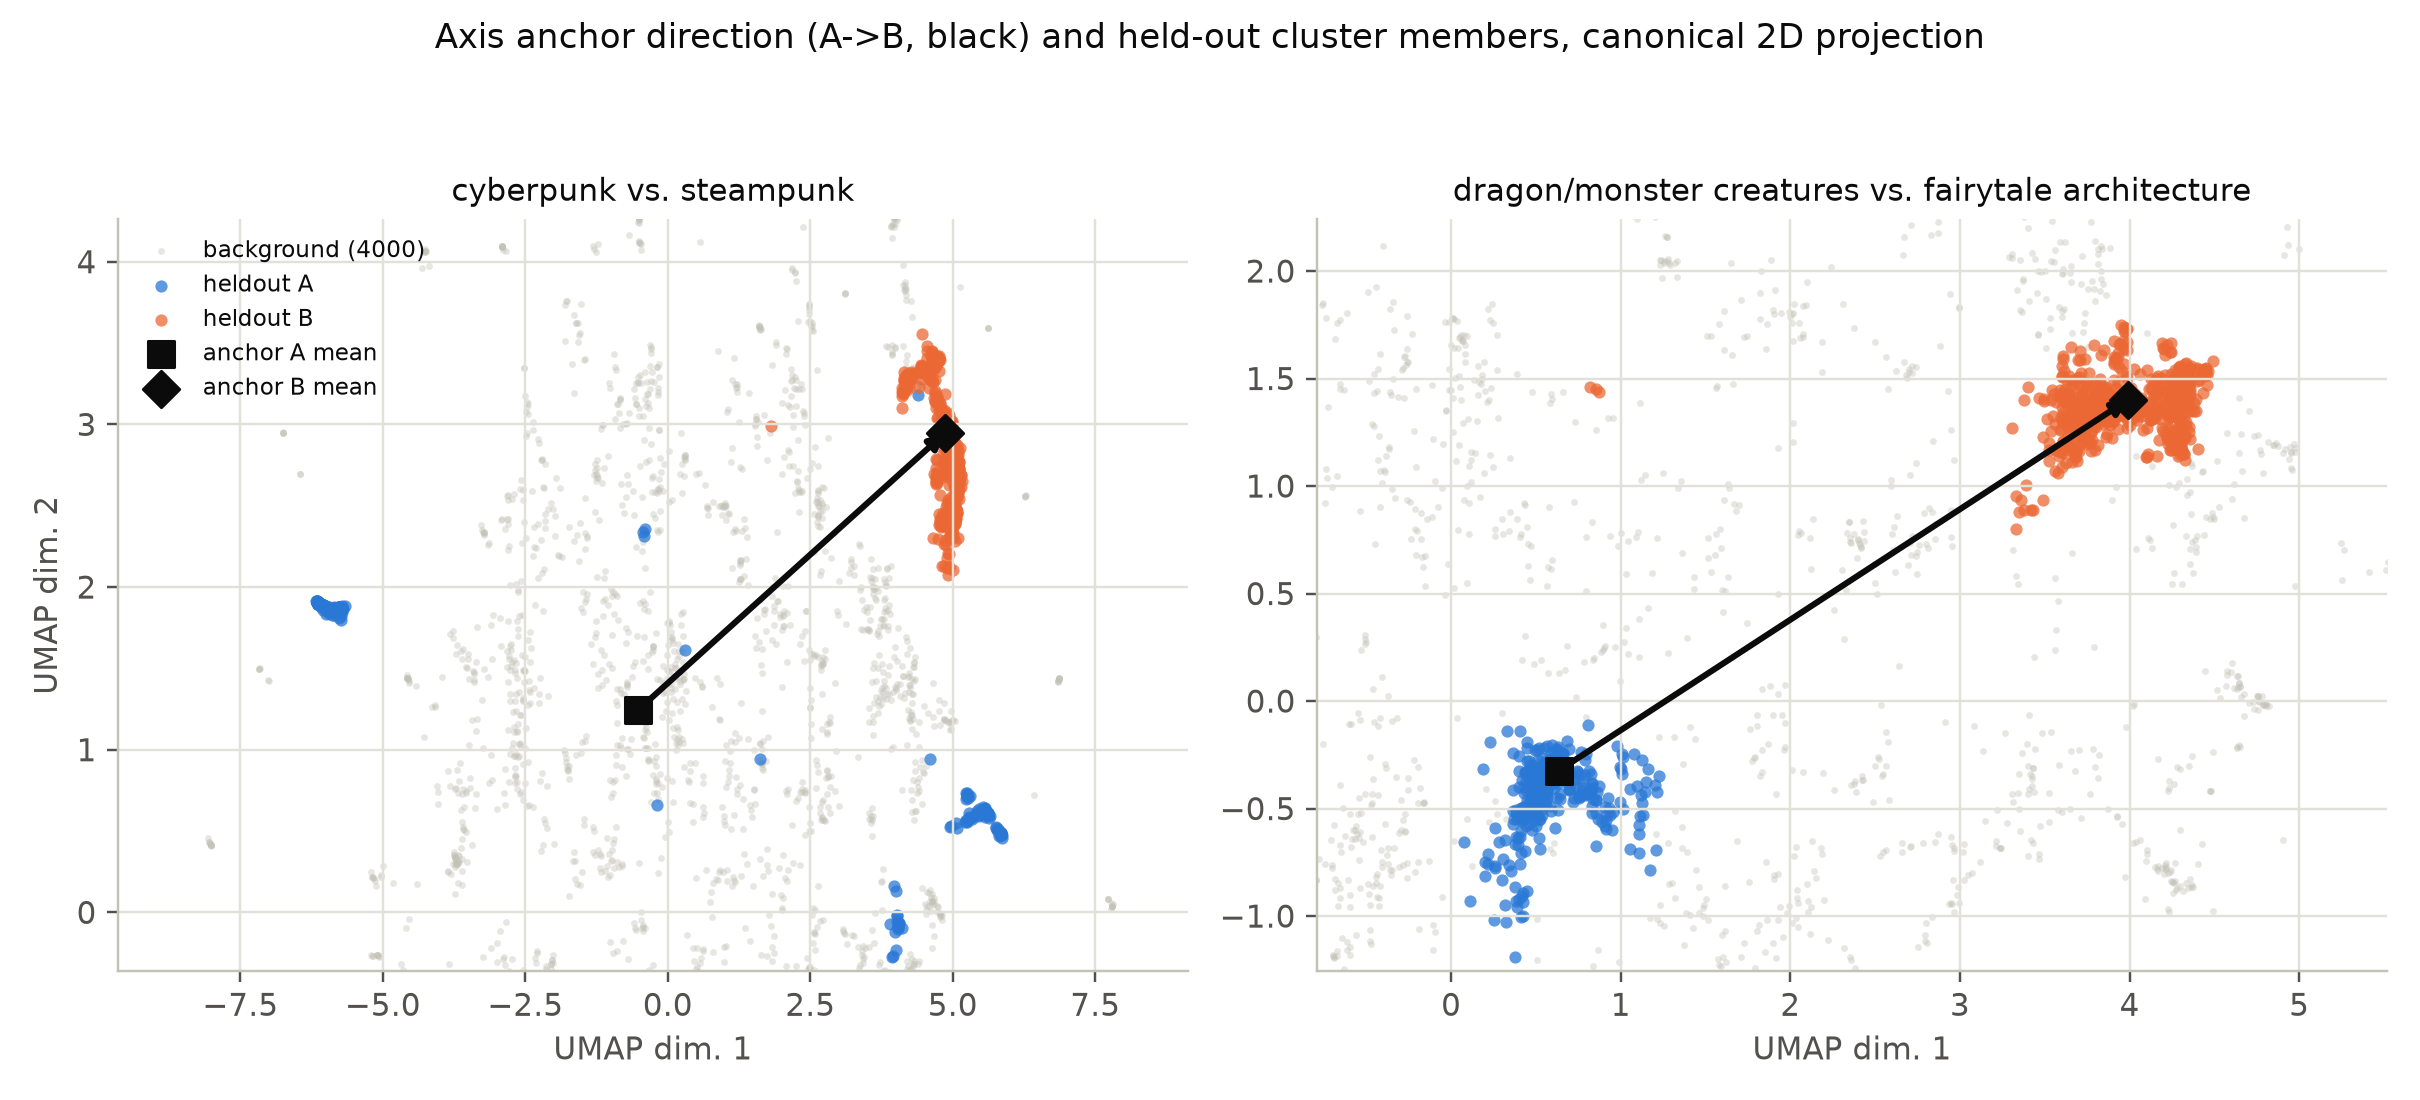
\includegraphics[width=0.7\textwidth]{figures/axis-projection-graph-2d.png}
\caption{Axis anchor direction (black arrow, between the two groups' 20-point anchor means) against held-out cluster members (blue/orange) and a 4.000-point background sample}
\label{fig:axis-projection-graph-2d}
\end{subfigure}
\begin{subfigure}[b]{\textwidth}
\centering
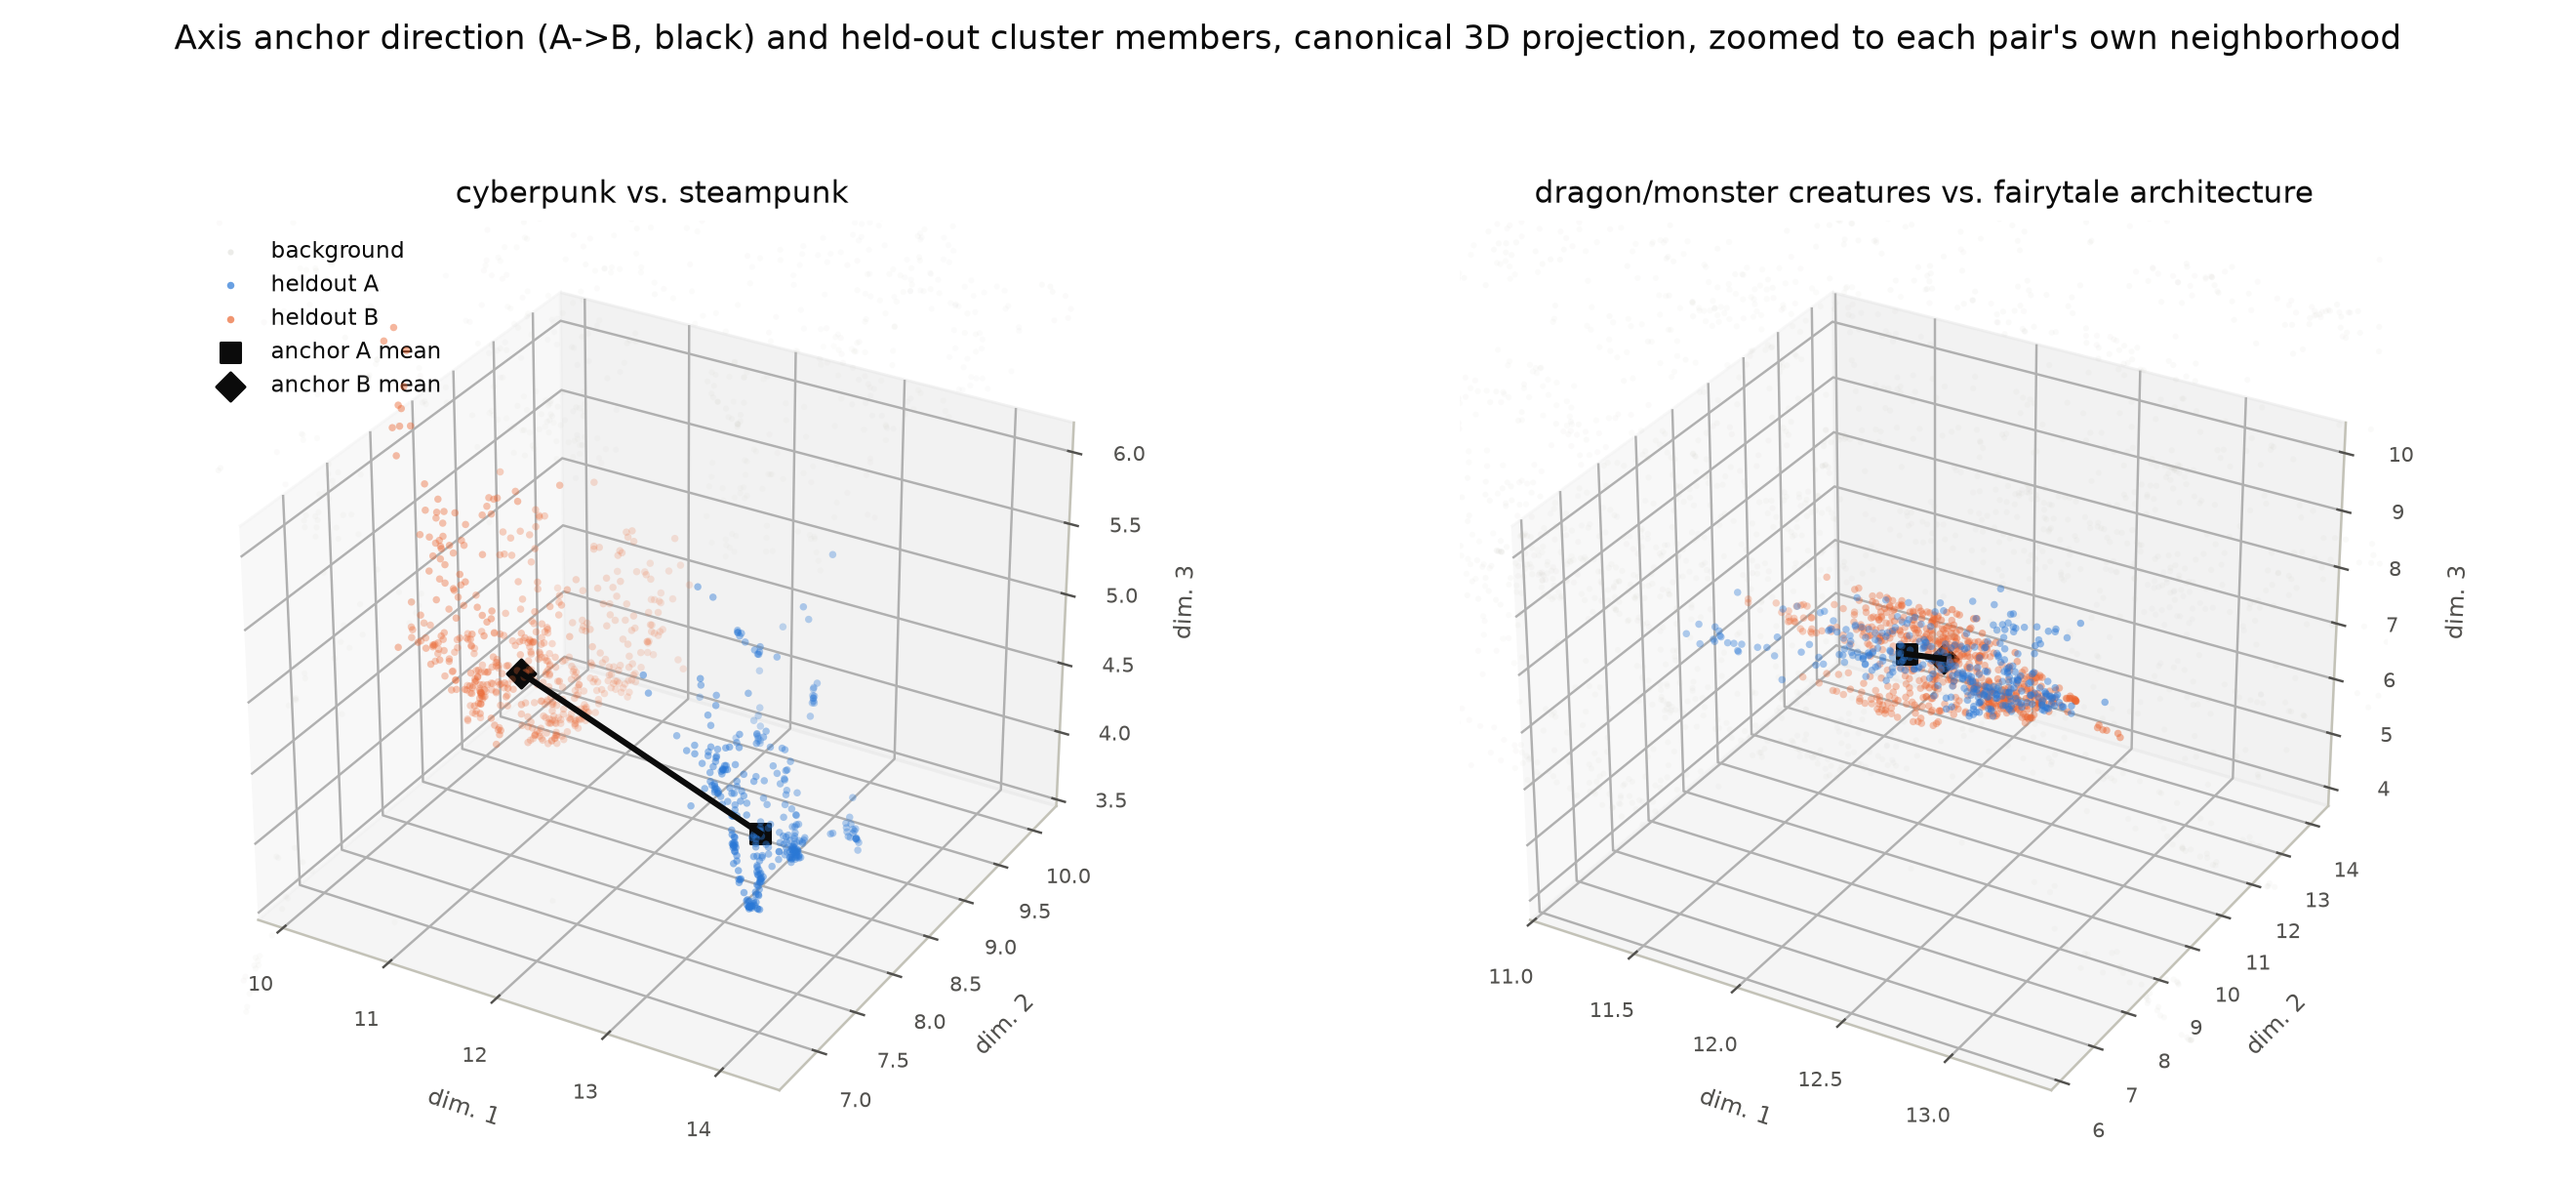
\includegraphics[width=0.7\textwidth]{figures/axis-projection-graph-3d.png}
\caption{The same two pairs in the 3D projection, axis limits zoomed to each pair's own held-out neighborhood}
\label{fig:axis-projection-graph-3d}
\end{subfigure}
\caption{Axis anchor direction and held-out cluster members, canonical 2D and 3D projection}
\label{fig:axis-projection-graph}
\end{figure}

The primary-axis score is computed in the compact embedding space rather than in the nonlinear UMAP display space. Its separation is therefore not guaranteed to remain visually apparent after projection. \hyperref[fig:axis-projection-graph-2d]{Figure~\ref*{fig:axis-projection-graph-2d}} and \hyperref[fig:axis-projection-graph-3d]{Figure~\ref*{fig:axis-projection-graph-3d}} show that it nevertheless remains visible for both pairs: held-out members of Groups A and B occupy distinct regions on opposite sides of the arrow connecting the anchor means. The three-dimensional view reveals an additional detail for pair 2. Although its groups appear clearly separated in two dimensions, some points overlap along their shared boundary when the third dimension is included. This suggests that part of the apparent 2D separation results from projection. The partial overlap for pair 2 does not conflict with its AUC of 1.000, because AUC is calculated from scores in the original compact space rather than from the reduced display coordinates. Overall, the thematic distinction remains visible after projection, although with some loss of clarity for pair 2.

For each pair, an automatically derived second axis was computed independently from the residual variation left after removing the primary axis. Both instances exceeded the 5 percent reporting threshold introduced in \hyperref[sec:4.8]{Section~4.8}, explaining 13.2 percent and 12.0 percent of the residual variance for pair 1 and pair 2 respectively, but their interpretation is less direct than that of the primary contrast. For pair 1, one extreme contains city and landscape prompts such as "steampunk city ... trending on artstation" and "good day, morning, landscape ... steampunk, forest, wood, lost world ...", while the other is dominated by named-character portraits such as "Loba from Apex Legends ... digital illustration portrait" or "Monica Bellucci as an angel", which could be interpreted as a scene-versus-portrait distinction. Pair 2 is less coherent, because one side combines "organic cyborg" and "organic mecha" prompts with an unrelated "city made of pages of paper" scene, whereas the opposite side again contains mainly named-character portraits. The three axis terms the operation derives for axis-2 ("detailed digital / style / full" vs. "steampunk / sharp / intricate" for pair 1 and "anime / detailed digital / trending artstation" vs. "focus / concept / sharp" for pair 2) are noticeably less informative than reading the underlying prompts directly, since single-word document-frequency terms cannot capture a composition-level distinction fully. The second axis should therefore be understood as simply the strongest remaining direction of variation after removing the primary contrast, not necessarily as another thematically related semantic dimension. This means, axis-2 is a much less reliable indicator of thematic structure than the primary axis, whose interpretation must be approached with more caution. Improving its interpretability, for example through additional constraints on the discovered direction or alternative axis-discovery techniques, remains an open direction for future work.

To summarize, a primary axis constructed from a small random set of anchors generalizes almost perfectly to unseen members of the same clusters, and its extracted axis terms also recover the intended thematic distinction. By contrast, the automatically discovered second axis satisfies the numerical reporting criterion but is substantially harder to interpret. Its meaning becomes noticeable mainly through inspection of the extreme prompts, revealing a gap between the structure detected by the operation and the explanation presented to the user.

\FloatBarrier
\section{Consistency Check}\label{sec:5.6}

\hyperref[sec:4.8]{Section~4.8} introduced Consistency Check as an operation that generates prompt variants at a configurable strength and evaluates their deviation from the base prompt using a consistency score and predicted cluster assignments. Because the operation changes both its generation mechanism and its LLM style tier as strength increases, this section examines whether the resulting scores remain continuous and well calibrated or whether these internal transitions introduce discontinuities.

Three base prompts of 6, 14, and 45 words, drawn from \texttt{imagenet1k\_labels\_classic} and \texttt{gustavosta\_sd\_prompts\_v2\_two\_pass}, were evaluated at seven variation strengths ranging (0.05, 0.2, 0.3, 0.35, 0.5, 0.7, 0.9), covering both generation mechanisms and all three style tiers. Five variants were generated per base prompt. Cluster stability, defined as the proportion of variants assigned to the same predicted cluster as the base prompt, was added as a second measure to examine the operation's stability from a different angle. Due to hardware constraints, Qwen2.5-3B-Instruct was used for paraphrase generation instead of the default Qwen2.5-7B-Instruct, which may have reduced the quality of the generated variants.

\begin{figure}[htbp]
\centering
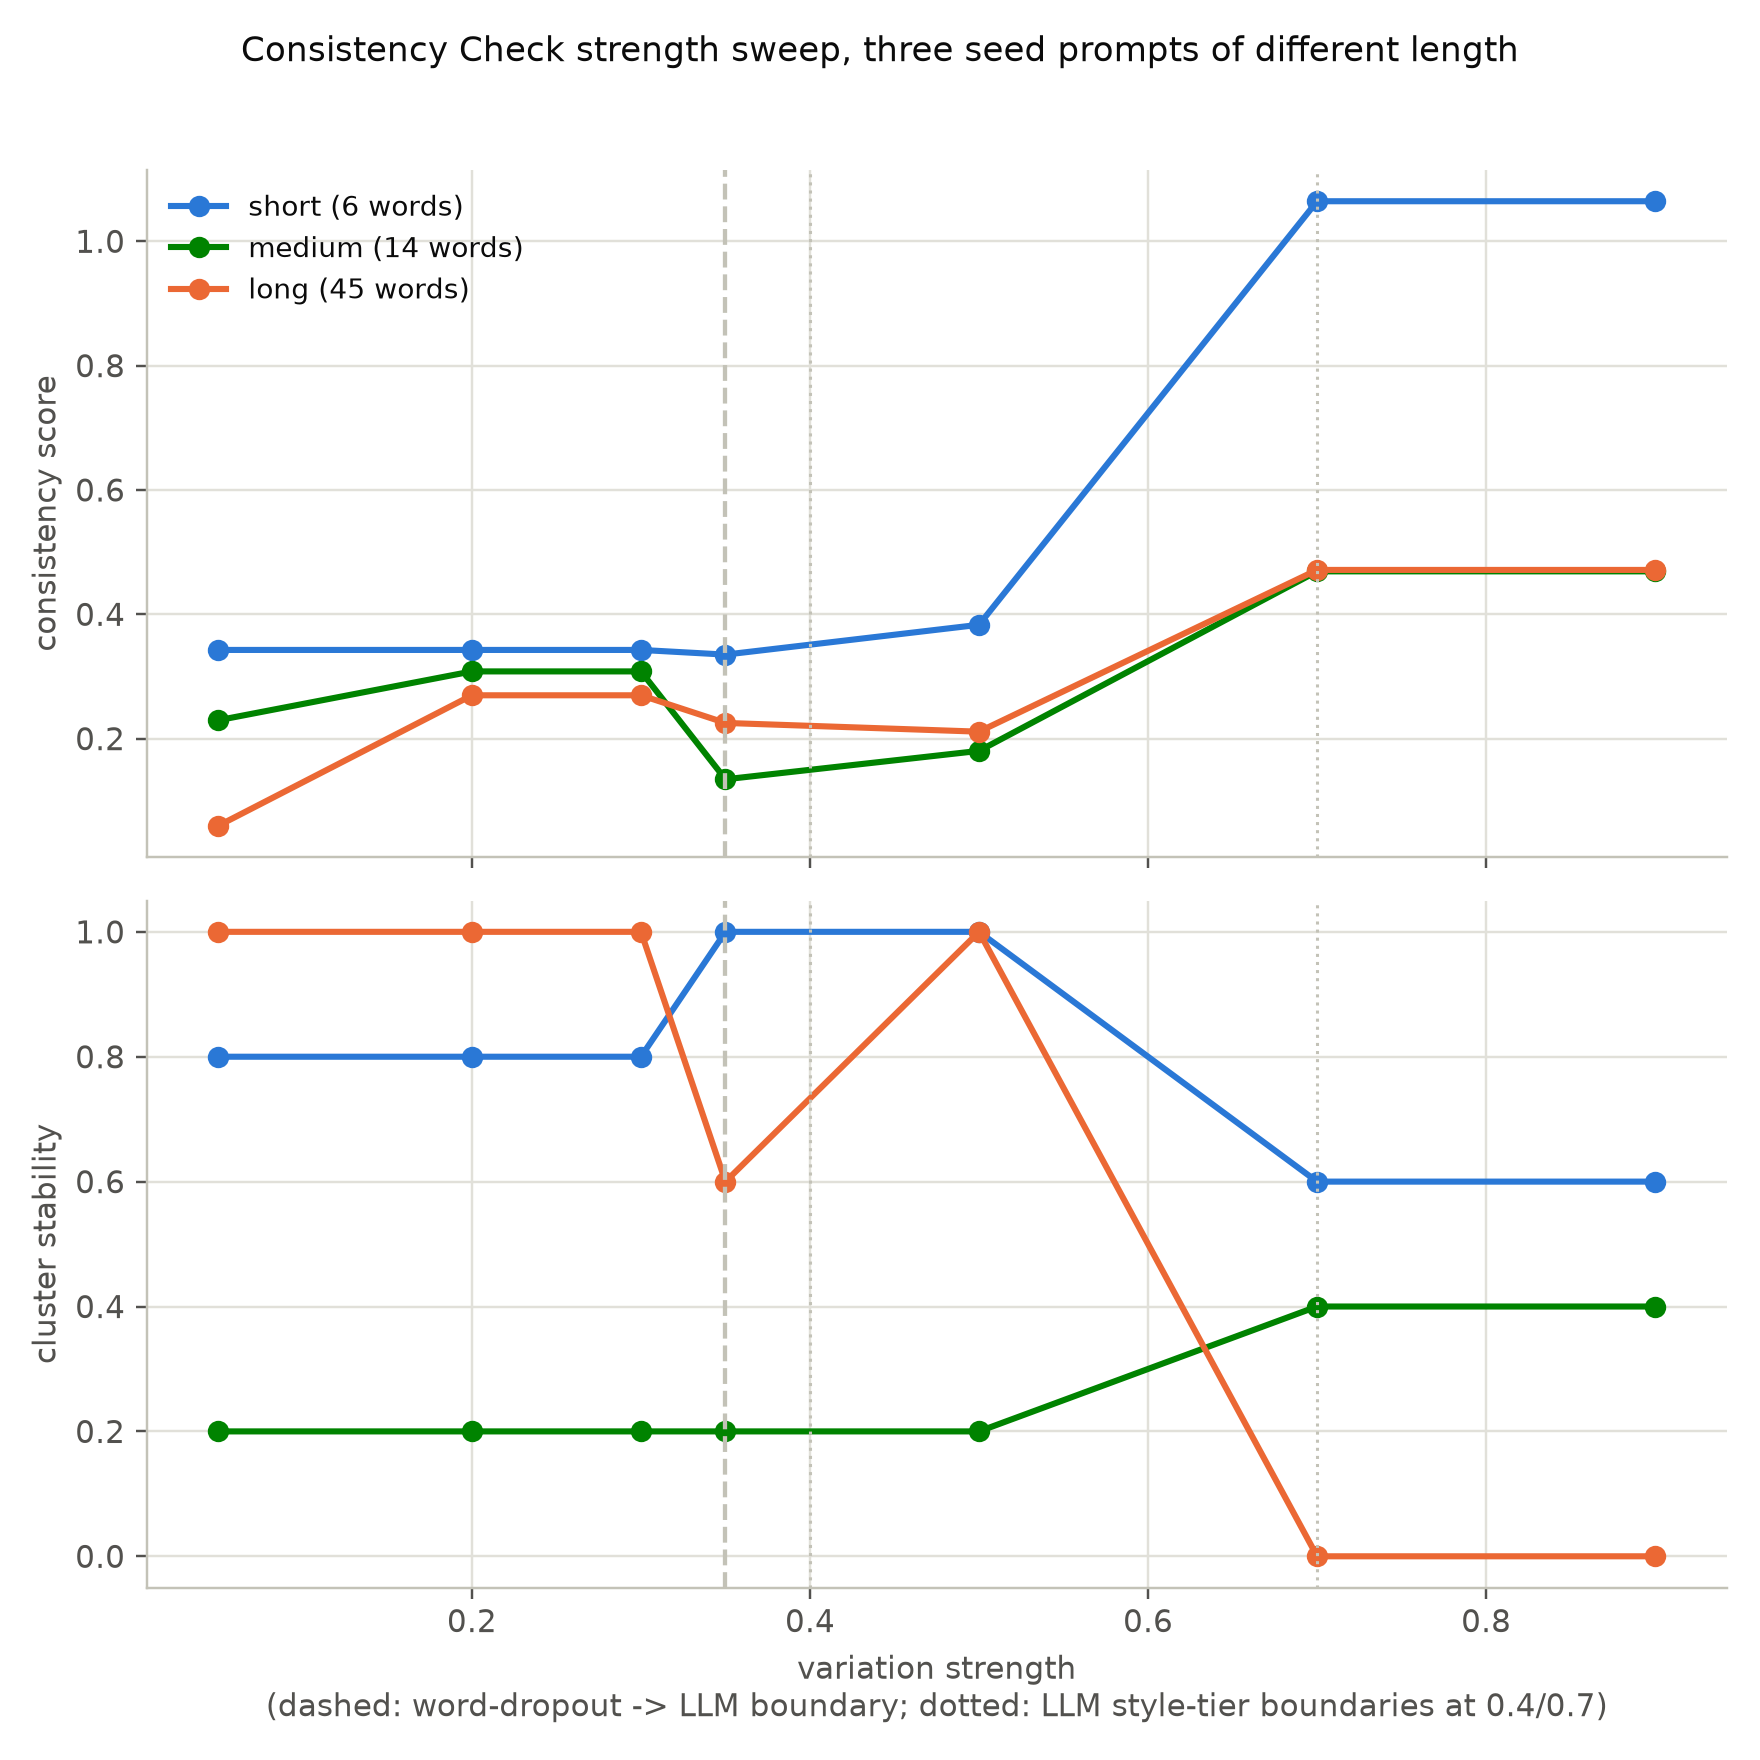
\includegraphics[width=0.79\textwidth]{figures/consistency-check-strength-sweep.png}
\caption{Consistency score and cluster stability across the strength sweep. Dashed line: word-dropout to LLM-paraphrase boundary. Dotted lines: LLM style-tier boundaries}
\label{fig:consistency-check-strength-sweep}
\end{figure}

As described in \hyperref[sec:4.8]{Section~4.8}, lower consistency scores indicate that the generated variants remain close to the base prompt, while higher values indicate greater drift. Although variation strength can be configured continuously, \hyperref[fig:consistency-check-strength-sweep]{Figure~\ref*{fig:consistency-check-strength-sweep}} shows that its practical effect is considerably more coarse. Below the mechanism boundary at 0.35, the dropout-count formula rounds to the removal of a single word for the short base prompt at strengths 0.05, 0.2, and 0.3. These settings therefore produce identical variants despite their different numerical values. At strengths of 0.7 and 0.9, all base prompts receive the same "substantial change" instruction. Combined with deterministic decoding, this results in identical LLM outputs at both settings.

The transition at 0.35 is also discontinuous. For the medium-length base prompt, the consistency score decreases from approximately 0.31 to 0.14 when the operation switches to the mechanism intended to produce stronger paraphrases. In addition, four of the twelve LLM-based runs did not return the required number of distinct variants and therefore invoked the base-prompt-copy padding fallback described in \hyperref[sec:4.8]{Section~4.8}. Since a copied base prompt has a cosine similarity of 1.0 by construction, this fallback artificially lowers the consistency score and increases cluster stability. This effect is attributable partly to the use of the smaller substituted language model rather than to the variation mechanism alone.

Cluster stability has a less systematic pattern and does not reliably follow the consistency score: although both are intended to reflect how far the variants have drifted from the base prompt, a rising or falling consistency score does not reliably correspond to a matching change in cluster stability. For the medium-length base prompt, stability remains at 0.20 through strength 0.5 even though the consistency score changes substantially. At each of these strengths, no more than one of the five variants remains in the base prompt's cluster 134, while the others are assigned mainly to the related cluster 27, as illustrated in \hyperref[fig:consistency-check-illustrative-strip]{Figure~\ref*{fig:consistency-check-illustrative-strip}}. Real semantic drift therefore does not necessarily produce corresponding changes in cluster stability.

The long base prompt exhibits the opposite pattern. Its cluster stability rises to 1.00 at strength 0.5 before falling to 0.00 at strengths 0.7 and 0.9, a change too large to be explained solely by the coarse resolution of five variants. This behavior is explained by the cluster-prediction mechanism classifying all variants as noise, rather than reassigning them to a different cluster. The consistency score and cluster assignment should therefore be understood as structurally different measures: one captures continuous displacement in embedding space, while the other records discrete movement across learned cluster boundaries. They may consequently diverge rather than change in parallel.

\begin{figure}[htbp]
\centering
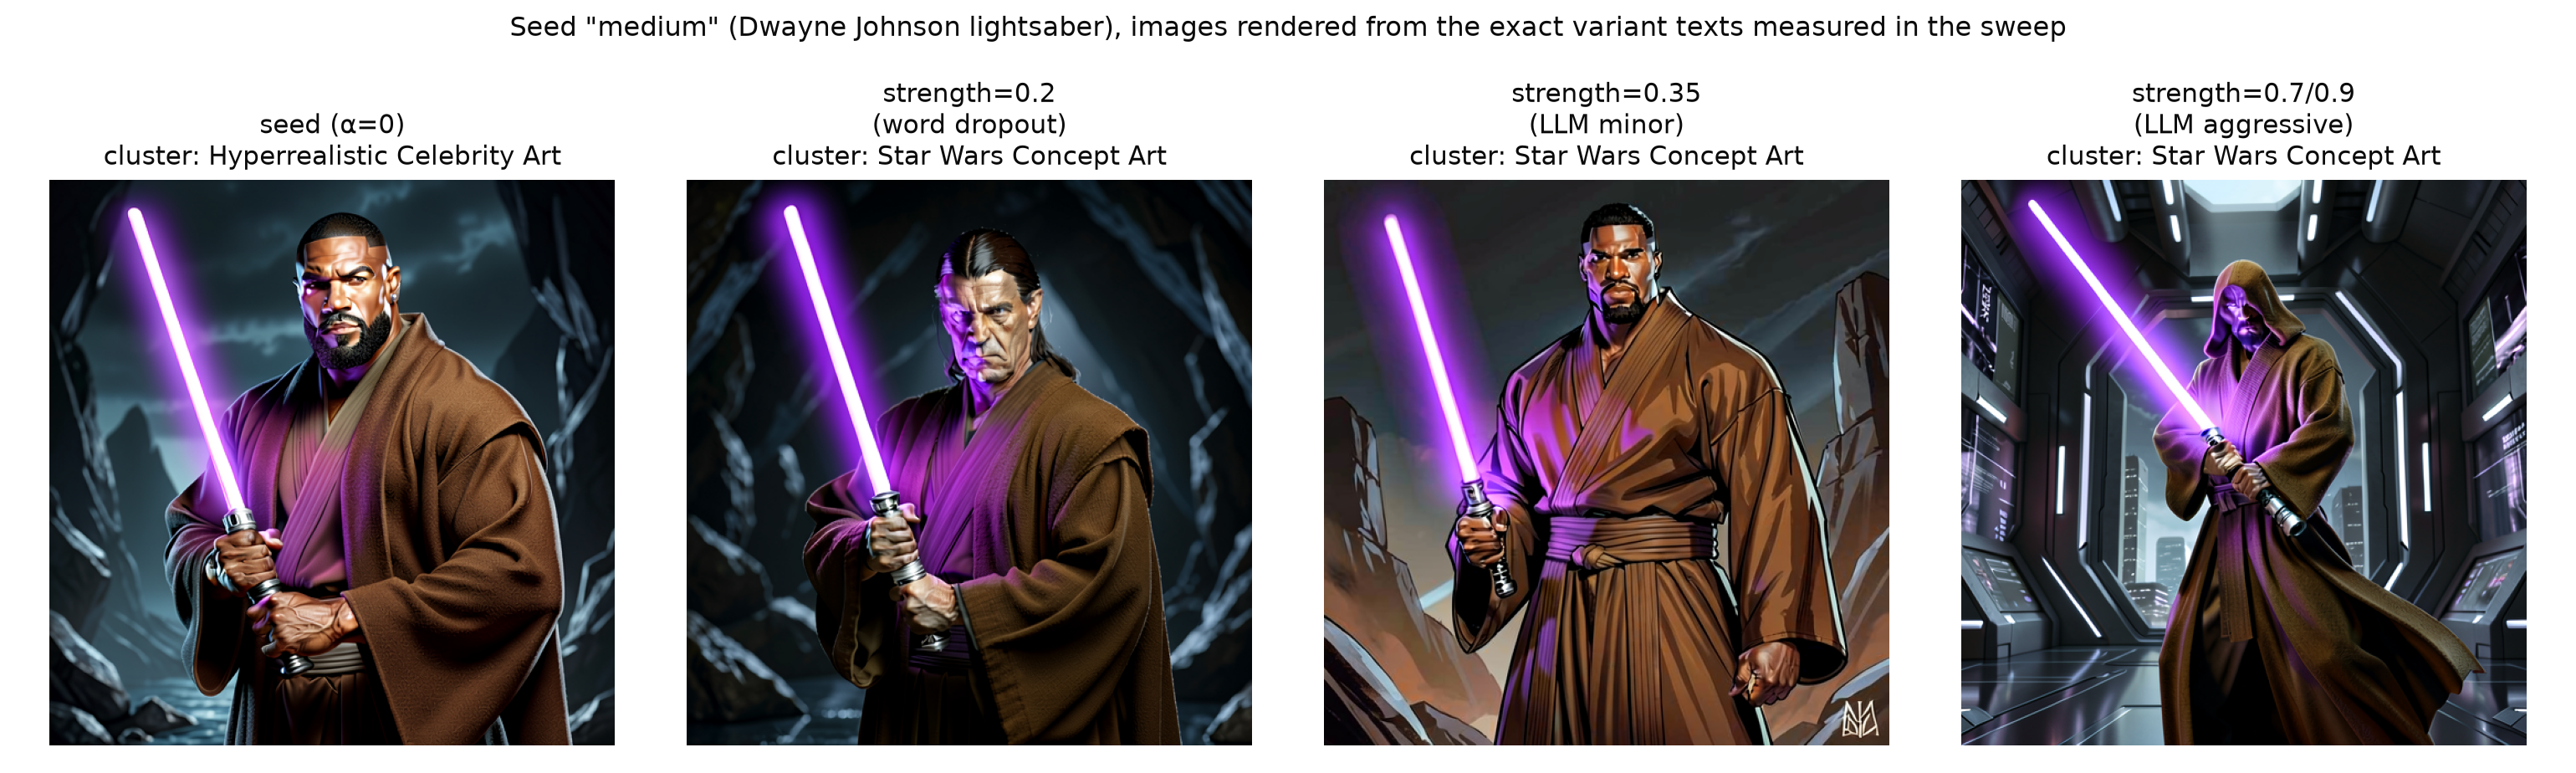
\includegraphics[width=\textwidth]{figures/consistency-check-illustrative-strip.png}
\caption{Base prompt "medium" (Dwayne Johnson lightsaber) rendered at its unmodified base prompt and three of its measured variants, spanning word dropout, LLM minor rewording, and LLM aggressive paraphrase}
\label{fig:consistency-check-illustrative-strip}
\end{figure}

The qualitative example in \hyperref[fig:consistency-check-illustrative-strip]{Figure~\ref*{fig:consistency-check-illustrative-strip}} supports both findings identified above: the coarse response of the consistency score and its limited correspondence with cluster stability. The figure renders the base prompt, "dwayne johnson holding a purple lightsaber wearing brown jedi robes, concept art, ultra realistic", together with three previously measured variants, so each variant's visual outcome can be compared directly against its own measured similarity to the base prompt. At strength 0.2, the word-dropout variant "holding a purple lightsaber wearing brown jedi robes, art, ultra realistic" removes the name "Dwayne Johnson" and eliminates the actor's likeness, although the consistency score remains on the same plateau as the other word-dropout conditions. At strength 0.35, the LLM minor-rewording variant "purple lightsaber in hand for dwayne johnson, brown robes, jedi style, ultra detailed concept art" preserves the name and recognizable identity while mainly altering the visual style. Nevertheless, the variant is reassigned from cluster 134 ("Hyperrealistic Celebrity Art") to cluster 27 ("Star Wars Concept Art"), suggesting that the cluster prediction is influenced more strongly by the lightsaber and Jedi-related content than by the celebrity reference. At strengths 0.7 and 0.9, the most aggressive paraphrase, "purple-hued lightsaber wielder in brown robes, futuristic concept, ultra-realistic art", removes the name, introduces an unrelated figure and setting, and remains in cluster 27. These examples show that neither the consistency score nor the cluster assignment alone provides a complete account of semantic stability.

Within this experiment, variation strength behaves more discretely than its continuous range suggests. Different structural causes produce this effect in the two generation mechanisms. As a result, even a small change in the numerical consistency score can coincide with a substantial shift in identity, subject, or scene. The findings are also specific to the use of Qwen2.5-3B-Instruct and may differ with another paraphrasing model. Differences across the three base prompts further indicate that prompt length and content influence plateau width and cluster behavior alongside the selected strength.

Consistency Check should therefore be interpreted as an exploratory estimate of stability rather than a definitive measure. Its coarse behavior follows directly from the current design, which combines integer word-dropout counts with a small number of discrete LLM style tiers. These choices make the operation simple and predictable, but limit fine-grained control. Future work could introduce more gradual dropout weighting or additional style levels to provide a more continuous response across the strength range.

\FloatBarrier
\section{Latent Probe}\label{sec:5.7}

\hyperref[sec:4.8]{Section~4.8} introduced Latent Probe as an operation that estimates a target embedding from a user-selected position in the projected space. The estimate, denoted $q$, is obtained by combining the compact embeddings of nearby reference points using inverse-distance weighting. It is then used for cluster prediction, nearest-prompt retrieval, and, optionally, an LLM-based search for a new prompt whose embedding lies close to $q$. \hyperref[sec:4.8]{Section~4.8} explicitly states that this is an exploratory approximation, not a claim of an exact recovery. The present section tests that claim directly by examining whether local geometry in the projection retains enough usable semantic information about the underlying prompt representations to support these tasks. Two held-out tests are used: Test A examines whether probing a point's true projected position reconstructs its original compact embedding, while Test B evaluates whether the LLM-based search can generate a new prompt that remains semantically close to the held-out source prompt.

Test A is performed on two datasets with substantially different levels of prompt diversity. The first uses \texttt{imagenet1k\_labels\_classic} and reuses the 800/200 split introduced in \hyperref[sec:5.2]{Section~5.2}. The split is applied directly to the dataset's existing coordinate and embedding arrays, with only the 800 training points made available as reference samples for inverse estimation. No projection model is refitted. Consequently, the stored coordinates of the 200 held-out points remain valid within the same coordinate system, avoiding the cross-fit alignment problem that required Procrustes analysis in \hyperref[sec:5.2]{Section~5.2}. The second dataset is \texttt{gustavosta\_sd\_prompts\_v2\_two\_pass}, the more diverse natural-language corpus used in the image-generation experiments. Here, 200 prompts are held out from the 61.746-point dataset, leaving 61.546 visible reference points.

For each held-out sample, the inverse-estimation procedure is evaluated at that sample's stored two- or three-dimensional position. The held-out point itself is excluded from the visible reference pool, and the operation estimates $q$ from the surrounding points. Recovery accuracy is measured by the cosine similarity between $q$ and the held-out sample's true compact embedding. Cluster recovery is measured by whether the cluster predicted from $q$ matches the held-out sample's canonical cluster label.

Because cosine-similarity values depend strongly on the dataset's overall embedding distribution, the results of both tests are interpreted relative to a dataset-specific background baseline, namely the mean cosine similarity between randomly paired prompts from the same dataset. Comparing the recovery values against this baseline makes it possible to judge them as a genuine signal rather than an artifact of how similar prompts in that dataset already tend to be by chance. For each corpus, 2.000 index pairs are drawn independently with replacement, meaning each draw is made from the full dataset again, so the same prompt can be selected more than once across different pairs from the full compact embedding matrix. Pairs containing the same sample twice are discarded, leaving 1.996 valid pairs for \texttt{imagenet1k\_labels\_classic} and 2.000 for \texttt{gustavosta\_sd\_prompts\_v2\_two\_pass}.

The resulting mean background similarity is 0.970 for ImageNet-1k, with a standard deviation of 0.018. This high value is partly explained by the shared prompt template "a photo of X." For the more varied natural-language dataset, the mean is lower at 0.901, with a standard deviation of 0.030. The precision of this kind of estimate depends on sample size rather than on what fraction of the dataset was sampled, so both baselines are equally reliable despite the datasets' very different sizes. The corresponding standard errors are approximately 0.0004 and 0.0007, both far smaller than the differences the following analysis relies on. Conceptually, this follows the same background-reference principle as the \texttt{mean inter} value used by Consistency Check in \hyperref[sec:4.8]{Section~4.8}, although here the baseline is used only for interpretation and does not affect the operation itself.

\begin{table}[htbp]
\centering
\caption{Test A held-out recovery, aggregated over 200 points per dataset}
\label{tbl:latent-probe-recovery}
\resizebox{\textwidth}{!}{%
\begin{tabular}{|l|l|c|c|}
\hline
\textbf{Dataset} & & \textbf{Recovery cosine (mean / median / SD)} & \textbf{Cluster match rate} \\
\hline
ImageNet-1k & 2D probe & 0.992 / 0.993 / 0.005 & 0.96 \\
\hline
ImageNet-1k & 3D probe & 0.993 / 0.994 / 0.004 & 0.98 \\
\hline
ImageNet-1k & random-pair baseline & 0.970 / 0.975 / 0.018 & -- \\
\hline
gustavosta & 2D probe & 0.974 / 0.977 / 0.017 & 0.79 \\
\hline
gustavosta & 3D probe & 0.977 / 0.981 / 0.016 & 0.84 \\
\hline
gustavosta & random-pair baseline & 0.901 / 0.905 / 0.030 & -- \\
\hline
\end{tabular}%
}
\end{table}

\begin{figure}[htbp]
\centering
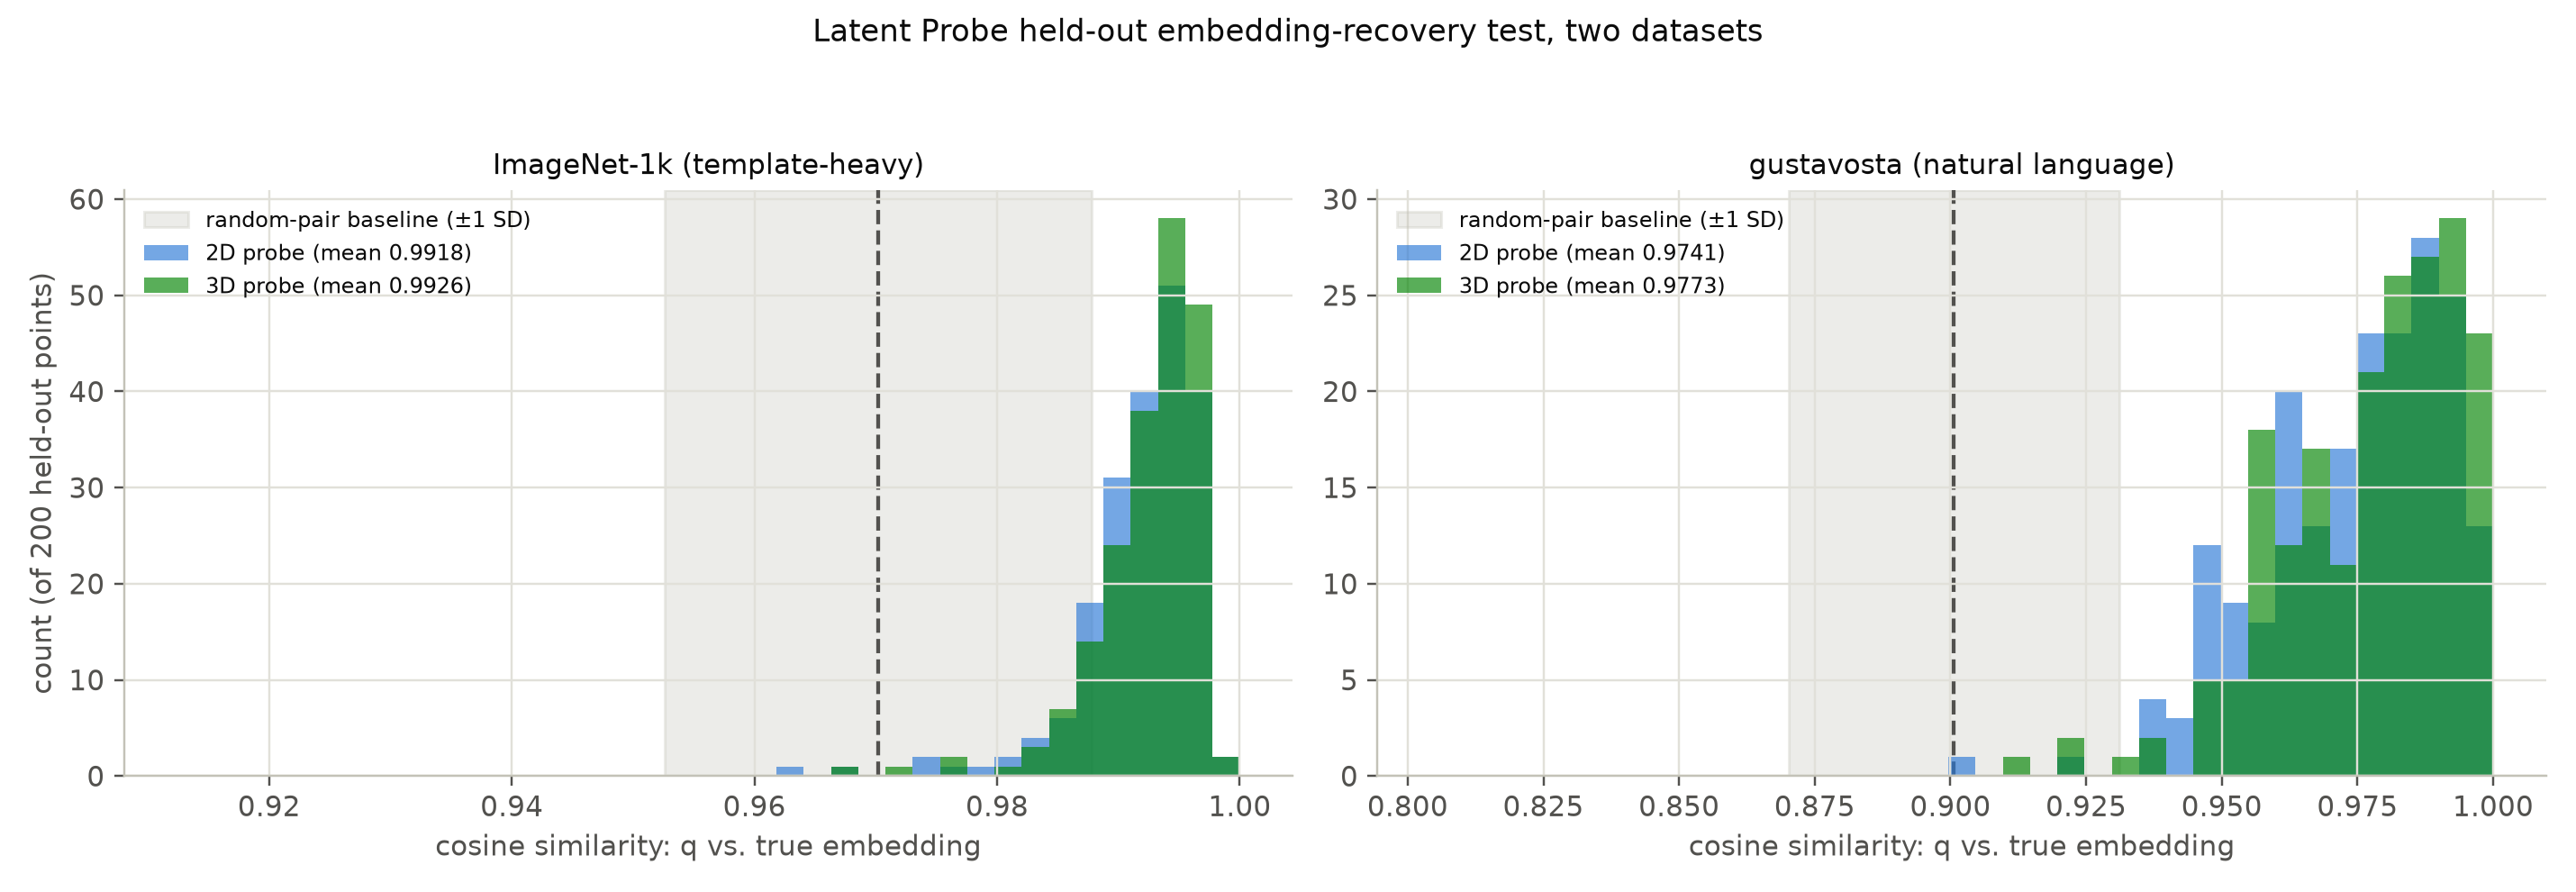
\includegraphics[width=0.9\textwidth]{figures/latent-probe-recovery-histogram.png}
\caption{Test A held-out recovery-cosine distribution against each dataset's own random-pair baseline band ($\pm$1 SD)}
\label{fig:latent-probe-recovery-histogram}
\end{figure}

\hyperref[tbl:latent-probe-recovery]{Table~\ref*{tbl:latent-probe-recovery}} and \hyperref[fig:latent-probe-recovery-histogram]{Figure~\ref*{fig:latent-probe-recovery-histogram}} show that recovery exceeds the random-pair baseline in both datasets, although by different margins. For ImageNet-1k, the mean recovery lies approximately 1.2-1.3 baseline standard deviations above the baseline mean, compared with about 2.4-2.5 standard deviations for \texttt{gustavosta\_sd\_prompts\_v2\_two\_pass}. The histograms further clarify how consistently individual points stay above the baseline by dataset. For gustavosta, very few of the 200 held-out samples fall inside the baseline range, meaning nearly every individual point is itself a genuinely strong recovery. For ImageNet-1k, a modest minority of points, 11 to 14 percent, still fall inside the range even though the large majority sits clearly above it, consistent with its narrower separation margin already noted above.

The clearer separation on the more diverse dataset is partly explained by the different baseline distributions. ImageNet-1k embeddings are already concentrated close to a cosine similarity of 1.0 because all prompts share the same template, as mentioned before, leaving relatively little room for recovery scores to separate from random pairs. The broader and lower baseline of the natural-language dataset makes the local-geometry signal easier to distinguish from chance. Greater prompt diversity therefore does not weaken recovery in this experiment, instead, it produces a more informative reference scale.

Recovery differs only marginally between the two- and three-dimensional probes, increasing from 0.992 to 0.993 for ImageNet-1k and from 0.974 to 0.977 for gustavosta. These differences are smaller than the variation within the recovery distributions and should not be interpreted as a meaningful advantage of the 3D representation.

Cluster recovery shows a different pattern. ImageNet-1k achieves cluster-match rates of 96 percent in 2D and 98 percent in 3D, whereas gustavosta reaches 79 percent and 84 percent, respectively. This lower result reflects a more demanding assignment problem: the natural-language dataset contains 141 clusters, with approximately 54 percent of its samples labeled as noise, while ImageNet-1k contains only about three clusters. It does not indicate weaker embedding recovery, since the same $q$ vectors still exceed their dataset-specific baseline by the larger margin. Several of the eight ImageNet-1k mismatches in 2D involve held-out samples whose canonical labels are noise, while $q$ is assigned to a nearby cluster instead. This is consistent with noise samples lying near cluster boundaries rather than indicating a distinct failure of the inverse-estimation procedure.

For Test B, six held-out ImageNet-1k samples were selected from the Test A results: the three with the lowest and the three with the highest recovery cosine. This allows reconstruction performance to be compared with the cases already identified as difficult or easy to recover. For each sample, the estimated vector $q$ from Test A was reused as the target of the LLM-based reconstruction search. The highest-ranked neighbors of $q$ served as seed prompts, while mid-ranked and distant points from the visible pool were used as noise and negative examples. The search followed the plugin's runtime configuration, using 15 seeds, 5 negative examples, 5 noise examples, and up to 10 refinement iterations or a 5-minute time limit.

Candidate prompts were generated and iteratively refined towards $q$. Reconstruction quality was evaluated using two cosine-similarity measures: the similarity between the reconstructed prompt's embedding and $q$, which indicates how closely the search reached its internal target, and the similarity between the reconstructed embedding and the held-out prompt's true embedding, which tests whether approaching $q$ also recovers the original representation.

\begin{table}[htbp]
\centering
\caption{Test B reconstruction for six held-out points (three with the lowest, three with the highest Test A recovery cosine)}
\label{tbl:latent-probe-reconstruction}
\resizebox{\textwidth}{!}{%
\begin{tabular}{|p{4.4cm}|p{4.4cm}|c|c|c|}
\hline
\textbf{True prompt} & \textbf{Reconstructed prompt} & \textbf{Recovery cos. (Test A)} & \textbf{cos. to q} & \textbf{cos. to true original} \\
\hline
a photo of gasmask, respirator, gas helmet & a photo of antique trolleybus, horse trolley, horse tramcar & 0.963 & 0.986 & 0.956 \\
\hline
a photo of tailed frog, bell toad, ribbed toad, tailed toad, Ascaphus trui & a photo of weathered ship's wheel & 0.968 & 0.950 & 0.907 \\
\hline
a photo of pick, plectrum, plectron & a photo of electric fan, desk fan, table fan & 0.974 & 0.989 & 0.964 \\
\hline
a photo of pillow & a photo of a hen with fluffy feathers & 0.998 & 0.989 & 0.988 \\
\hline
a photo of volleyball & a photo of a basketball hoop with players & 0.998 & 0.989 & 0.989 \\
\hline
a photo of baseball & a photo of a radiator with colorful flames & 0.998 & 0.990 & 0.988 \\
\hline
\end{tabular}%
}
\end{table}

\hyperref[tbl:latent-probe-reconstruction]{Table~\ref*{tbl:latent-probe-reconstruction}} reflects the same division observed in Test A. The three points with the lowest recovery cosine also yield the lowest similarities between reconstructed and original embeddings, ranging from 0.907 to 0.964, all below the ImageNet-1k random-pair baseline of 0.970. In contrast, the three strongest recoveries achieve similarities of 0.988-0.989, clearly above baseline. Despite this numerical difference, none of the six reconstructed prompts describes the same object as the original. For example, "a photo of pillow" becomes "a photo of a hen with fluffy feathers," while only "a photo of volleyball" and "a photo of a basketball hoop with players" retains a loose categorical relation. High cosine similarity therefore does not imply close topical correspondence: proximity in the compact embedding space and similarity in described content are related, but not equivalent. All six searches converged within the first beam, as no subsequent refinement improved the initial candidates beyond the configured threshold.

Test B is limited to six deliberately selected ImageNet-1k samples and was not repeated on \texttt{gustavosta\_sd\_prompts\_v2\_two\_pass}, since its qualitative conclusion, close embedding similarity does not imply close described content, is a property of the reconstruction search itself rather than one expected to depend strongly on which dataset supplies the target. The selected points were chosen to span the recovery range observed in Test A rather than to form a representative random sample. In addition, the plugin's default paraphrasing model was replaced because of the 8 GB GPU-memory constraint described in \hyperref[sec:5.6]{Section~5.6}. The exact wording of what got reconstructed is therefore specific to this particular LLM, because different models have different word choices, biases, and creative tendencies, and a different model would very plausibly phrase things differently or even land on entirely different candidate objects altogether.

Overall, the estimated target vector recovers a held-out point's embedding and cluster context more accurately than the corresponding random-pair baseline, with the stronger relative separation occurring on the more diverse dataset. The reconstruction search also follows the point-specific pattern predicted by Test A: better estimates of $q$ lead to embeddings closer to the original. Answering this section's opening question, local geometry in the projection therefore does carry usable semantic information, in the sense of recovering an embedding and cluster context close to the original, but it does not preserve or encode which specific object or topic that embedding actually describes. This supports the interpretation of Latent Probe as an exploratory navigation tool rather than a reconstruction method.
